\documentclass[12pt,a4paper]{article}
\usepackage{graphicx}
\usepackage{xcolor}
\usepackage[english]{babel}
\usepackage[utf8]{inputenc}
\usepackage{mathtools}
\usepackage{amsmath}
\allowdisplaybreaks
\usepackage{amssymb}
\usepackage{geometry}
%\usepackage{cite}
\usepackage{tikz}
\usepackage{float}
\usepackage[sorting=none, sortcites]{biblatex}
\addbibresource{references.bib}
\usepackage{verbatim}
\usepackage{autobreak}
%\usepackage{algorithm} 
\usepackage[english, ruled, vlined]{algorithm2e}
%\usepackage{algpseudocode} 
\usepackage{circuitikz}
%\usepackage{rubikcube,rubikrotation,rubikpatterns,rubiktwocube}
\usepackage{amsthm}
\graphicspath{ {./images/} }
\newtheoremstyle{custom}% name
{15pt}% Space above
{5pt}% Space below
{\itshape}% Body font
{}
{\bfseries}% Theorem head font
{}% Punctuation after theorem head
{\newline}% Space after theorem head
{}% Theorem head 

\theoremstyle{custom}
\newtheorem*{proposition}{Proposition}
\newtheorem*{definition}{Definition}
\newtheorem*{lemma}{Lemma}
\newtheorem*{theorem}{Theorem}
\newtheorem*{corollary}{Corollary}
\newtheorem*{proofcustom}{Proof}
\newtheorem*{note}{Note:}
\newtheorem*{example}{Example}
\newtheorem*{notation}{Notation:}

\usepackage[nottoc]{tocbibind}

\usepackage[onehalfspacing]{setspace}
\usetikzlibrary{positioning,arrows.meta}
\usepackage{stmaryrd}

\usepackage{microtype}

\usepackage{booktabs}

\usepackage{array}
%\usepackage{hyperref}
%\hypersetup{colorlinks,allcolors=black}
%\usepackage{hyperref}
%\hypersetup{
    %colorlinks=true,
   % linkcolor=black,
    %filecolor=black,      
    %urlcolor=blue,
   % citecolor=black
%}


\usepackage{subfigure}

\usepackage[compact]{titlesec}     


\usepackage[center]{caption}


\pagestyle{plain}

%\usepackage[backend=biber, maxbibnames=99]{biblatex}

%\addbibresource{references.bib}

\usepackage{adjustbox}

\newcommand{\Gtwo}{\ensuremath{G_{2\times 2\times 2}}}

\newcommand{\Gthree}{\ensuremath{G_{3\times 3\times 3}}}

\newcommand{\Ttwo}{2$\times$2$\times$2-}

\newcommand{\Tthree}{3$\times$3$\times$3-}

\clubpenalty = 10000
\widowpenalty = 10000
\displaywidowpenalty = 10000


\geometry{
  paper=a4paper, 
  top=3cm, % Top margin
  left=2cm, % Left margin
  right=3cm, % Right margin
  %showframe, % Uncomment to show how the type block is set on the page
}

\setlength{\parindent}{0em}

\setlength{\parskip}{1.3ex}




\title{Group Theory of the \\ 2$\times$2$\times$2 Rubik's cube and its solution algorithms}
\author{Riddhiman Bhattacharya}







\begin{document}

\begin{titlepage}
    \centering
    %\includegraphics[width=0.4\textwidth]{VB.png}\par\vspace{1cm}
   % {\scshape\LARGE Visvabharati University \\ Santiniketan\par}
    %\vspace{1cm}

    {\huge\bfseries \textcolor{blue}{Group Theory of \\ 2$\times$2$\times$2 Rubik's Cube \\ and \\ Its Solution Algorithms}\par}
    \vspace{2cm}
    {\Large\itshape Riddhiman Bhattacharya\par}
    \vspace{2cm}
     \includegraphics[width=0.5\textwidth]{images/2x2scrambled.png}\par\vspace{1cm}
    \vfill
   % B.Sc: UG-I
    %supervised by\par
    %Prof.~First \textsc{Last}

    \vfill

% Bottom of the page
    {\large May 9, 2024 \par}
\end{titlepage}



\setcounter{page}{1}


\newgeometry{
  top=2.5cm, % Top margin
    left=2cm, % Left margin
  right=3cm % Right margin
}



\newgeometry{
  top=3cm, % Top margin
  left=2cm, % Left margin
  right=3cm % Right margin
}


%\setstretch{1.5}
\thispagestyle{empty}
\thispagestyle{empty}\tableofcontents\thispagestyle{empty}\thispagestyle{empty}
\clearpage
\newpage

\thispagestyle{empty}
\begin{abstract}
   The \Tthree cube is the subject of numerous works and is examined several times as a group \cite{JC,TD,DDJT,DJ,RMG,TR}. Not only that, 
The \textit{God's Number} (the maximum required number of rotations of the optimal solution path) is the subject of many works and has often been calculated and improved by new algorithms \cite{Godgrol,salkinder2021n,RMG,Hu,TR,doi:10.1137/120867366,MMFAA}. 
The calculation of the \textit{God's Number} of the \Tthree cube is much more demanding and therefore also more interesting than that of the \Ttwo cube. The motivation of this work is to apply the knowledge of the \Tthree cube in \Ttwo cube. In contrast to the \Tthree cube, the \Ttwo cube has fewer pieces and no edge cubies - this makes the smaller cube less complex. However, the \Ttwo cube can be rotated due to the lack of center cubies, which means that the top side can be changed at will. In this work, the knowledge of the group of the \Tthree cube is adapted and thus the \Ttwo cube is represented using group theory to gain knowledge about the cube which includes calculating the number of possible cube configurations and creating a concept for finding the optimal solution path. 
\end{abstract}
\clearpage



\newpage
\pagenumbering{arabic}
\pagestyle{plain}

\section{Introduction}
Rubik's Cube \footnote{These few texts and articles give us some glimpse into the history and popularity of rubik's cube \cite{pekonen2021cubed, demaine2011algorithms,2018ChJME..31...77Z,bandelow1982inside,Hofstader,singmaster1980notes} }, designed by Ern\H{o} Rubik, is a $3D$ permutation puzzle \cite{wong2010group}. The concept of Rubik's Cube is thought to be originated from the Chinese Luo book that can be simplified into a zero-dimensional $3^{rd}$ order cube called Jiugong Map \cite{2018ChJME..31...77Z}.

\begin{definition} Certain configuration that has to be formed by the combination of $n^2$ numbers, i.e. {$1,2,3,..., n^2$} numbers in n-order square that makes the sum of the numbers in each row, column and two diagonal lines a constant value. That constant is called the \textbf{magic square constant} \cite{zen} and is given by $$\boxed{\frac{n(n^2+1)}{2}}$$
\end{definition}
\begin{itemize}
    \item Magic Square Constant for 2 - order cube: 5
    \item Magic Square Constant for 3 - order Cube : 15
\end{itemize}

\begin{figure}[h]
\centering
\includegraphics[scale=0.5]{Models_of_R-Cube.png}
\caption{Models of Rubik's Cube \cite{2018ChJME..31...77Z}}
\label{Figure_Mrubik's cube}
\end{figure}
\subsection*{Permutation Puzzle}
\label{PP}
\begin{definition}
    A \textbf{permutation puzzle} is a one-person game that follows the properties \cite{wong2010group} : 
    \begin{itemize}
        \item Depending on the structure of the puzzle for some $n>1$, each move leads to a unique puzzle position \footnote{Puzzle Position is defined as an element in set generated by all possible legal moves.}, so, the function $f: \text{moves} \Rightarrow \text{Puzzle Positions}$ is a bijective mapping in $P= 1,2,...,n$.
        \item Each move must be invertible, that for some move $M$, $\exists$ $M^{-1}$ that restores the puzzle to the position it was before the move $M$ was performed. 
        \item If $f_1(M_1)=P_1$ and $f_2(M_2)=P_2$, then either $M_1 \mathlarger{\scriptstyle*}M_2$ [performing moves in sequence] is not a legal move or corresponds to the permutation of function composition ${f_1} \mathlarger{\scriptstyle*}{f_2}$ 
        
    \end{itemize}
\end{definition}






There are many more interesting readings and paper on origin of permutation (combinatorics) puzzles \cite{BIGGS1979109} and history of Rubik's cube \cite{pekonen2021cubed}. We'll now dive more into \Ttwo cube and \Tthree cube now. 


\section{Terminology and Basic Features}
\fbox{\textbf{\Ttwo Cubes}} \\

Also called \textbf{Pocket Cube}, the cube is made up of eight smaller cubes.
In Figure \ref{Figure_CubeUnsolvedSolved}, it can be seen on the left in the twisted state and on the right in the solved state. 
In the starting configuration (also basic position, initial position) of the \Ttwo cube, each side has four coloured areas of the same colour.

\begin{figure}[h]
\centering
\includegraphics[scale=0.1]{2x2scrambled.png}
\includegraphics[scale=0.1]{2x2solved.png}
\caption[Unsolved and Solved \Ttwo cube]{Unsolved and Solved \Ttwo cube}
\label{Figure_CubeUnsolvedSolved}
\end{figure}
\fbox{\textbf{\Tthree Cubes}}\\

Much popular than the \Ttwo cube  is the \Tthree cube. It consists of 27 small cubes [26 of them are visible, and $27^\text{th}$ cube [cubie] doesn't exist actually]. 
\newpage
In Figure \ref{Figure_3erCube} it can be seen unsolved on the left and in the starting configuration on the right.

\begin{figure}[h]
\centering
\includegraphics[scale=0.11]{3x3_sc_so.png}
\caption[Unsolved and solved \Tthree cube]{Unsolved and solved \Tthree cube}
\label{Figure_3erCube}
\end{figure}

\fbox{\textbf{$n\times n \times n$ Cube}}\\

It is an extension of \Tthree cube which takes the form of $n\times n \times n$ cube made out of $1 \times 1\times 1$ pieces and each $n\times n \times 1$ is free to rotate around its center. 
\begin{figure}[H]
\centering
\includegraphics[scale=0.6]{7X7X7.png} \hspace*{2em}
\includegraphics[scale=0.66]{6X6X6.png}
\caption{Cubie types for odd and even n \cite{salkinder2021n} \\ a) Cubie types for a $7\times 7 \times 7$
Rubik’s Cube  b) Cubie types for a $6 \times 6 \times 6$ Rubik’s Cube. }
\label{nnn}
\end{figure}

\subsection{Terminology}


 \begin{definition}
        The individual small cubes that make up a cube are \textbf{Cubies}.
        
    \end{definition}
    \textbf{Example: } 
    \begin{enumerate}
        \item The \Ttwo cube has 4 cubies in each face.
        \item The \Tthree cube has 9 cubies in each face.
    \end{enumerate}
    
    
 \begin{definition}
     Each cubies has one, two, three visible faces called \textbf{facelets}.
 \end{definition}

 \begin{note}
 Based on the no of facelets in case of \Tthree cube, cubie can be divided into \textit{centre-cubie: One facelet}, \textit{edge-cubie: two facelet} and \textit{Corner-Cubie}

\begin{center}
\begin{tabular}{|c|c|}
\hline
\textbf{Type of Cubie} & \textbf{Facelet(s)} \\
\hline
\textit{Centre-Cubie} & One facelet \\
\hline
\textit{Edge-Cubie} & Two facelets \\
\hline
\textit{Corner-Cubie} & Three facelets \\
\hline
\end{tabular}
\end{center}
 
 \end{note}
 
 \begin{definition}
        The space where the cubies reside is \textbf{Cubicle}. 
    \end{definition}

\begin{note}
   \textbf{Cubies vs Cubicles:} Cubicles are named the same way as cubies but represent the positions in space where the cubies reside rather than the physical blocks, If the cubie is solved, then \textbf{each cubie resides in the cubicle} that has the same name as it. When moves are applied to the cube, cubies can move and occupy other cubies but the cubicles are fixed in space \cite{wein2011mathematics}.
\end{note}
    \begin{definition}
        The positions occupied by facelets are called \textbf{slots}.
    \end{definition}
    
\begin{definition}
    A \textbf{state of the cube} is a bijection mapping 
    $$\boxed{
\text{\{facelets\}} \xrightarrow{\cong} \text{\{slots\}}
}$$
\end{definition}
  In case of \Tthree cube, there are 54! states \cite{anu}. And, in case of \Ttwo cube, there are 24! states. \\
\textbf{So, to generalize for } $n \times n \times n$ \text{ cube, we've } $6n^2$ $\text{! states.}$


\begin{definition}
    The initial arrangement of the Rubik's Cube where each face is has a solid colour and each facelet belongs to one and only one face is the Starting / Initial configuration. \end{definition}


\subsection{Basic Feature of Rubik's Cube} 
\subsubsection{Symmetry Characteristic}
In mathematics, the concept of symmetry is described and explained by group theory. 
If an operation executed on a system transforms the system from one state to another state, and the two states are equivalent, then the system is symmetric to this operation.

Rubik’s cube has axial symmetries of four orders, two orders
, and three orders and is symmetric about the body center at the same time \cite{Hu,singmaster1980notes}.


\begin{figure}[H]
\centering
\includegraphics[scale=0.5]{Symmetry.png}
\caption{The axial symmetries of (a) four orders, (b) two orders, and (c) three orders in Rubik’s cube. [Source: \cite{Hu}]}
\label{symm}
\end{figure}

\subsubsection{Combinatorial Characteristics}
Every state of the Rubik’s cube, whether solved or scrambled, can be achieved by rotating consecutively the six faces of the cube in solved position in finite steps, and can be restored by rotating the faces back step by step. The calculation which I'll be doing here is pretty simple \footnote{There are some nice explanations and discussions in \cite{hoda2010finding, animesh2018calculating, JC, 2018ChJME..31...77Z}}. 


\textbf{The puzzle was originally advertised as having over 3,000,000,000 combinations but only one solution}. Even Ern\H{o} Rubik mentioned in his autobiography: "\textit{It was as if I were staring blankly at a secret code, which I had created but could not penetrate}".
Depending on how combinations are counted, the actual number is significantly higher.
The original \Tthree Rubik's Cube has eight corners and twelve edges. There are $8!= 40,320$ ways to arrange the corner cubes. 
And $12!$ ways to arrange the edge cubies. Each corner cubie has 3 possible orientations, so $3^8$ ways of orienting the corner cubies and each edge cubies has 2 possible orientations, so $2^{12}$ possibilities of orienting the edge cubies, total nunmber of possible permutations  is

$$\boxed{8! \times 12!\times 3^8 \times 2^{12} \approx 5.19 \times 10^{20}}$$

This huge number has both valid and invalid configurations. I've discussed this in detail in Section \ref{Chapter_ValidConfigurations}. 

We've to find the number of valid configurations. 
So, for that we know each corner has three possible orientations, although only seven (of eight) can be oriented independently; the orientation of the $8^\text{th}$ corner depends on the preceding seven, giving $3^{7}= 2,187$ possibilities.
There are $12!/2 (239,500,800)$ ways to arrange the edges, restricted from 12! because edges must be in an even permutation exactly when the corners are. (When arrangements of centres are also permitted, as described below, the rule is that the combined arrangement of corners, edges, and centres must be an even permutation \cite{Hu}.) Eleven edges can be flipped independently, with the flip of the twelfth depending on the preceding ones, giving $2^{11}= 2,048$ possibilities \cite{wong2010group}.\\

\begin{center}
    $\boxed{8! * 3^{7} * \frac{12!}{2} * 2^{11}  = 43,252,003,274,489,856,0000}$
\end{center}
which is approximately $43$ quintillion.
Given any one of
the 43,252,003,274,489,856,000 states, it is possible to return to the solved state in 20
moves or less! That’s why 20 is called God’s Number [Discussed in section \ref{God}].
\subsubsection{Cycle Characteristic}
One of the basic but interesting characteristics is its cyclic nature. 
When we twist and turn the cube in a repeating pattern, it goes through a cycle. Basically, the idea is that the Rubik's cube is executed through a certain
number of moves /operations from the original state back to the original state again, thus achieving a cycle. The cycle characteristic of moves operation can be
divided into two categories: \textbf{periodic} and \textbf{non-periodic} based on the circulation period [$C_p$] (\textit{The number of the times the Rubik's Cube is rotated.})
If the $C_p$ is constant- the cycle is \textbf{periodic} and if $C_p$ is variable, then the cycle is non-periodic. The sequence of operations of a \textbf{non-periodic} cycle is
based on both the sequence of periodic cyclic operations
and the \textbf{“constant process”} [\textit{Refers to
the fact that all pieces can return to their original state
after this sequence of operations.}] that causes the cube’s pattern to exhibit a non-periodic change.


\subsection{Singmaster Notation}

\begin{figure}[H]
\centering
\includegraphics[scale=0.5]{SingNotation.png} \\
\caption{Singmaster Notation [Source: \cite{singmaster1980notes}]}
\label{Sing}
\end{figure}


The following table describes the basic features of the cube.

\begin{center}
\begin{tabular}{|c|c|c|}
\toprule
\textbf{Moves} & \textbf{Abbreviation} & \textbf{Description} \\
\midrule
\textbf{Front} & $F$ & Side currently facing the person \\
\textbf{Back} & $B$ & Side opposite of the Front \\
\textbf{Up} & $U$ & Side above/on top of the front side \\
\textbf{Down} & $D$ & Side opposite the top, underneath the cube \\
\textbf{Right} & $R$ & Side directly to the right of front \\
\textbf{Left} & $L$ & Side directly to the left of front \\
\bottomrule
\end{tabular}
\end{center}
\begin{center}
\begin{tabular}{|c|c|}
\hline
\textbf{Rotation} & \textbf{Description} \\
\hline
x & Rotate the entire cube on R \\
\hline
y & Rotate the entire cube on U \\
\hline
z & Rotate the entire cube on F\\
\hline
\end{tabular}
\end{center}
\begin{figure}[H]
\centering
\includegraphics[scale=0.95]{notation.png} \\
\caption{Rubik's Cube Notation}
\label{Intro moves Sing}
\end{figure}


\subsection{Naming a Cubie}
\label{Name}




The division of the cube positions is shown in the figures \ref{Image_cubiePositionName} and \ref{Cubie pos. folded out}. The individual cubie positions are named with the abbreviations that describe their position with \textit{up, down, right, left, front} and \textit{back}.

\begin{minipage}[b][][b]{0.04\textwidth}$\ $
\end{minipage}\begin{minipage}[b][][b]{0.43\textwidth}

\begin{figure}[H]
\centering
\includegraphics[scale=0.15]{caged_positions.png} \\
\caption[Names of the cubies  positions in the cube]{Cubies positions in the cube}
\label{Image_cubiePositionName}
\end{figure}

\end{minipage}\begin{minipage}[b][][b]{0.06\textwidth}$\ $ \end{minipage}\begin{minipage}[b][][b]{0.43\textwidth}

\begin{figure}[H]
\centering
\includegraphics[scale=0.2]{foldedout_cage.png}
%\includegraphics[scale=0.15]{foldedout_cage_color.png}%
\caption[Cube folded out with the names of the cubie positions]{Cube folded out with the Cubies position}
\label{Cubie pos. folded out}
\end{figure}

\end{minipage}\begin{minipage}[b][][b]{0.04\textwidth}$\ $ \end{minipage}

In Figure \ref{Image_cubiePositionName} the names of the cubie positions on the cube are shown. In Figure \ref{Cubie pos. folded out} the cube can be seen in unfolded form. 

Each cubie position is assigned a unique name to identify it. This assumes that the white side is at the top in the starting configuration and the red side is at the front. The cubie positions are described with 3 letters, which consist of the abbreviations \textit{u, d, r, l, f, b}. These abbreviations stand for \textit{up, down, right, left, front, back}. \\
For example, the cubie position at the top left front is called \textit{ulf} (for \textit{up}, \textit{left} and \textit{front}).
\begin{note}
    \begin{itemize}
        \item Each cubie also gets a unique name that corresponds to its position when scrambled. 
        \item Sometimes we've to care which face has to be listed first- these are \textbf{Oriented Cubies}. For those cubies $urf$, $fur$, $rfu$ are different.\\
\textbf{Corner cubies are labeled by listing the facelets in clockwise order looking from the corner to the middle of the cube.}
        
\item In other cases, we don't care which face is listed first, so, that is \textbf{Unoriented Cubies}. 

\end{itemize}
\end{note}
A detailed discussion that I've not talked here can be found in this really interesting text \cite{lutterworth}. 


\section{Configuration of the Cube}
\label{Chapter_ConfigurationOfCube}

To work with the cube, we must determine the position it is in.
So, for a \Ttwo  cube, configuration is made up of two parameters :
\begin{itemize}
\item Position of the corner cubies (specified as $\sigma$)
\item Orientation of corner cubies (specified as $x$)
\end{itemize}
The configuration of the cube can be written as a 2-tuple: $(\sigma, x)$.
The position of the corner cubies is defined as a set of bijective functions $\sigma$ and the orientation of the corner cubies is defined as a vector $x$.

The idea and conceptualization of the \Tthree cube configuration is nicely discussed in \cite{JC,lutterworth}. Here, I've tried working the same for the \Ttwo cube. In contrast to the \Tthree cube, the \Ttwo cube only requires two instead of four configuration parameters. This means that the position and orientation of the edge cubies are not taken into account.

I've tried explaining the change of cube configuration step by step using an example move.

\subsection{Positions of the Cubies in the Cube}

\label{Section_PositionsOfThecubiesInTheCube}

The set of bijective functions $\sigma$ (for each rotation of the face) contains functions that represent the transitions of the cube pieces. The transitions describe the change in the position of the cubies during a move. The function $\sigma$ maps each cube position to a new position, this is a permutation mapping.


Now, to illustrate, the permutation $\sigma_U$ is defined for a rotation of the upper layer by 90$^\circ$ clockwise. 
Here, $\sigma_U$ is described in details and different notations are given. The derivation of the further rotations works analogously.
The rotation of the upper layer is shown graphically in the figures \ref{Figure_CubiePositionNameAfterU-1} and \ref{Figure_CubiePositionNameAfterU-2}.


\begin{figure}[h]
\begin{minipage}[b][][b]{0.04\textwidth}$\ $
\end{minipage}\begin{minipage}[b][][b]{0.43\textwidth}

\begin{figure}[H]
\centering
\includegraphics[scale=0.15]{caged_spin.png}\\
\caption{Cubie positions in the cube after move $U$}
\label{Figure_CubiePositionNameAfterU-1}
\end{figure}

\end{minipage}\begin{minipage}[b][][b]{0.06\textwidth}$\ $ \end{minipage}\begin{minipage}[b][][b]{0.43\textwidth}

\begin{figure}[H]
\centering
\includegraphics[scale=0.15]{foldedout_spin.png}
\caption{Folded out cube with cubie positions after move $U$}
\label{Figure_CubiePositionNameAfterU-2}
\end{figure}

\end{minipage}\begin{minipage}[b][][b]{0.04\textwidth}$\ $ \end{minipage}
\end{figure}

In Figure \ref{Figure_CubiePositionNameAfterU-1}, we can see that the cubies of the lower layer have not been moved. The upper layer positions have shifted one cubie clockwise. This results in the following function $\sigma_U$:
\begin{alignat*}{4}
& \sigma_U(\textit{ulf})=\textit{ulb} \ \ \ \ \ \ \ && \sigma_U(\textit{ulb})=\textit{urb} \ \ \ \ \ \ \ && \sigma_U(\textit{urb})=\textit{urf} \ \ \ \ \ \ \ && \sigma_U(\textit{urf})=\textit{ulf} \\
& \sigma_U(\textit{dlf})=\textit{dlf} \ \ \ \ \ \ \ && \sigma_U(\textit{dlb})=\textit{dlb} \ \ \ \ \ \ \ && \sigma_U(\textit{drb})=\textit{drb} \ \ \ \ \ \ \ && \sigma_U(\textit{drf})=\textit{drf} 
\end{alignat*}
The notation of the form $i \mapsto j$ is also common:
\begin{alignat*}{4}
& \textit{ulf} \mapsto \textit{ulb} \ \ \ \ \ \ \ \ && \textit{ulb} \mapsto \textit{urb} \ \ \ \ \ \ \ \ && \textit{urb} \mapsto \textit{urf} \ \ \ \ \ \ \ \ && \textit{urf} \mapsto \textit{ulf} \\
& \textit{dlf} \mapsto \textit{dlf} \ \ \ \ \ \ \ \ && \textit{dlb} \mapsto \textit{dlb} \ \ \ \ \ \ \ \ \ && \textit{drb} \mapsto \textit{drb} \ \ \ \ \ \ \ \ && \textit{drf} \mapsto \textit{drf} 
\end{alignat*}

This results in the following cycles: $\sigma_U = \ ( \textit{ulf} \ \textit{ulb} \ \textit{urb} \ \textit{urf} )\ ( \textit{dlf} )\ ( \textit{dlb} )\ ( \textit{drb} )\ ( \textit{drf} )$

Single-element cycles do not need to be written down. Then, the cycle $\sigma_U = \ ( \textit{ulf} \ \textit{ulb} \ \textit{urb} \ \textit{urf} )$. This cycle describes the transition of cubie positions as the upper layer is rotated.


The rotations of all layers can be described by the following cycles:
\begin{align*}
\sigma_U & =\ ( \textit{ulf} \ \textit{ulb} \ \textit{urb} \ \textit{urf} ) \\
\sigma_D & =\ ( \textit{dlf} \ \textit{drf} \ \textit{drb} \ \textit{dlb} ) \\
\sigma_F & =\ ( \textit{ulf} \ \textit{urf} \ \textit{drf} \ \textit{dlf} ) \\
\sigma_B & =\ ( \textit{ulb} \ \textit{dlb} \ \textit{drb} \ \textit{urb} ) \\
\sigma_L & =\ ( \textit{ulb} \ \textit{ulf} \ \textit{dlf} \ \textit{dlb} ) \\
\sigma_R & =\ ( \textit{urb} \ \textit{drb} \ \textit{drf} \ \textit{urf} ) 
\end{align*}

The indices on the functions $\sigma$ represent the various basic moves of the cube. 

The identity permutation is written as $\sigma=1$. This corresponds to the permutation of the empty move, which can be formed from other basic moves. I've explained it in section \ref{Section_EqualityOfmoves}.
Thus, the permutation of the empty move is defined as follows:
\begin{align*}
\sigma_N = 1
\end{align*}

\subsection{Orientation of the Cubies}
 \label{Section_AlignmentOfcubies}
The \Ttwo cube consists of eight corner cubies, each with three coloured areas. This means that each cubie has three possible orientations.
To recognize the alignment of the cubies, the cube positions on a coloured area are assigned a number. To do this, the white and yellow coloured cubies are marked and numbered. These numbers are referred to as $x_i$ with $i \in \lbrace 1, 2, 3, 4, 5, 6, 7, 8 \rbrace$. $x_1$ corresponds to position 1, $x_2$ corresponds to position 2, etc. This is shown on the left in Figure \ref{MarkingX}.

In addition, each cubie is assigned a number on each coloured area. Since, each cubie can have three orientations, the coloured areas are numbered 0, 1 and 2. The numbering starts with the white or yellow area at 0 and then counts the areas clockwise. This is shown on the right in Figure \ref{MarkingX}.
In the starting configuration all $x_i = 0$, the vector $x$ is then $(0, 0, 0, 0, 0, 0, 0, 0)$. This is written as $x=0$ for short.
\begin{figure}[H]
\centering
\includegraphics[scale=0.15]{foldedout_numbers.png} \hspace*{2em}
\includegraphics[scale=0.15]{foldedout_012.png}
\caption[Markings $x_i$ (left), colour area numbers (right)]{Unfolded cube with markings for $x_i$ (left) and coloured area numbers (right)}
\label{MarkingX}
\end{figure}


The following is an example of the move $R$ and the change in the colour area numbering is shown for illustration (Figure \ref{Figure_XaftermoveR}). $R$ is a rotation of the right face by 90$^\circ$ clockwise.
The labels $x_{1-8}$ remain in the same position. The numbering of the coloured areas changes as the face rotates, allowing the corner cubie alignment to be assigned.
The left side of the cube is not affected. Therefore, the faces at positions $x_1, x_3, x_5, x_7$ are all 0 because they are assigned to the left half of the cube.
The other positions of $x$ now show different colour areas:
\begin{align*}
x_2 = 2 \ \ \ \ \ \ x_4 = 1 \ \ \ \ \ \ x_6 = 1 \ \ \ \ \ x_8 = 2
\end{align*}
Therefore, $x = (0, 2, 0, 1, 0, 1, 0, 2)$ after move $R$ is made. This can also be seen from Figure \ref{Figure_XaftermoveR}. On the left are the positions of the vector entries of $x$ and on the right, we can see the cube with the coloured area numbering after the move $R$ has been made.
\begin{figure}[H]
\centering
\includegraphics[scale=0.13]{foldedout_012_white.png} \hspace*{2em}
\includegraphics[scale=0.13]{foldedout_012_spin.png}
\caption[Left: $x_1$ to $x_8$, right: change after move $R$]{Left: Positions $x_1$ to $x_8$, right: Change of the Numbered Corner Cubies after move $R$}
\label{Figure_XaftermoveR}
\end{figure}

Using the example move $R$, a function $\Gamma_R$ can be set up for each vector entry, which describes the change in the vector $x$ after executing the move $R$ for any initial configuration. Since $x_1, x_3, x_5$ and $x_7$ are not affected, they remain unchanged. The vector entry that is changed into the subsequent value by $\Gamma_R$ is highlighted in black below. All other entries are grayed out.
\begin{align*}
& \Gamma_{R_1}(\textcolor{gray}{(\textcolor{black}{x_1}, x_2, x_3, x_4, x_5, x_6, x_7, x_8  )})=\textcolor{gray}{(\textcolor{black}{x_1}, x_2, x_3, x_4, x_5, x_6, x_7, x_8  )} \\
& \Gamma_{R_3}(\textcolor{gray}{(x_1, x_2, \textcolor{black}{x_3}, x_4, x_5, x_6, x_7, x_8  )})=\textcolor{gray}{(x_1, x_2, \textcolor{black}{x_3}, x_4, x_5, x_6, x_7, x_8  )} \\
& \Gamma_{R_5}(\textcolor{gray}{(x_1, x_2, x_3, x_4, \textcolor{black}{x_5}, x_6, x_7, x_8  )})=\textcolor{gray}{(x_1, x_2, x_3, x_4, \textcolor{black}{x_5}, x_6, x_7, x_8  )}\\
& \Gamma_{R_7}(\textcolor{gray}{(x_1, x_2, x_3, x_4, x_5, x_6,\textcolor{black}{x_7}, x_8  )})=\textcolor{gray}{(x_1, x_2, x_3, x_4, x_5, x_6, \textcolor{black}{x_7}, x_8  )} 
\end{align*}
The surfaces at positions $x_2, x_4, x_6$ and $x_8$ are changed depending on the previous cubie orientations. The following function results for the positions $x_2$ after the move $R$:


\begin{align*}
\Gamma_{R_2}(\textcolor{gray}{(x_1, \textcolor{black}{x_2}, x_3, x_4, x_5, x_6, x_7, x_8  )})= \begin{cases}
\textcolor{gray}{(x_1, \textcolor{black}{2}, x_3, x_4, x_5, x_6, x_7, x_8  )} & \ \text{falls } x_4 = 0 \\ 
\textcolor{gray}{(x_1, \textcolor{black}{0}, x_3, x_4, x_5, x_6, x_7, x_8  )} & \ \text{falls } x_4 = 1 \\
\textcolor{gray}{(x_1, \textcolor{black}{1}, x_3, x_4, x_5, x_6, x_7, x_8  )} & \ \text{falls } x_4 = 2 
\end{cases}
\end{align*}
The function $\Gamma_{R_2}$ changes the vector entry $x_2$ after executing the move $R$ depending on the vector entry $x_4$. The coloured area that reaches position $x_2$ by executing the move is directly dependent on the coloured area at position $x_4$, since it is the same cubie. If there is initially a colour area with value 0 at position $x_4$, executing $R$ will bring the color area with value 2 of the same cubie to position $x_2$. This can also be seen in Figure \ref{Figure_Transition functionR}. This works analogously with $x_4 = 1$ (then $x_2 = 0$) and $x_4=2$ (then $x_2 = 1$).

\begin{figure}[H]
\centering
\includegraphics[scale=0.13]{TransitionfunctionR.png}
\caption{Change of $x_2$ with move $R$}
\label{Figure_Transition functionR}
\end{figure}

The other functions for changing the vector $x$ are also defined by the dependence of the cubie surfaces on each other.
\begin{align*}
\Gamma_{R_4}(\textcolor{gray}{(x_1, x_2, x_3, \textcolor{black}{x_4}, x_5, x_6, x_7, x_8  )})= \begin{cases}
\textcolor{gray}{(x_1, x_2, x_3, \textcolor{black}{1}, x_5, x_6, x_7, x_8  )} & \ \text{falls } x_8 = 0 \\ 
\textcolor{gray}{(x_1, x_2, x_3, \textcolor{black}{2}, x_5, x_6, x_7, x_8  )} & \ \text{falls } x_8 = 1 \\
\textcolor{gray}{(x_1, x_2, x_3, \textcolor{black}{0}, x_5, x_6, x_7, x_8  )} & \ \text{falls } x_8 = 2 
\end{cases} \\
\\
\Gamma_{R_6}(\textcolor{gray}{(x_1, x_2, x_3, x_4, x_5, \textcolor{black}{x_6}, x_7, x_8  )})= \begin{cases}
\textcolor{gray}{(x_1, x_2, x_3, x_4, x_5, \textcolor{black}{1}, x_7, x_8  )} & \ \text{falls } x_2 = 0 \\ 
\textcolor{gray}{(x_1, x_2, x_3, x_4, x_5, \textcolor{black}{2}, x_7, x_8  )} & \ \text{falls } x_2 = 1 \\
\textcolor{gray}{(x_1, x_2, x_3, x_4, x_5, \textcolor{black}{0}, x_7, x_8  )} & \ \text{falls } x_2 = 2 
\end{cases} \\
\\
\Gamma_{R_8}(\textcolor{gray}{(x_1, x_2, x_3, x_4, x_5, x_6, x_7, \textcolor{black}{x_8})})= \begin{cases}
\textcolor{gray}{(x_1, x_2, x_3, x_4, x_5, x_6, x_7, \textcolor{black}{2})} & \ \text{falls } x_6 = 0 \\ 
\textcolor{gray}{(x_1, x_2, x_3, x_4, x_5, x_6, x_7, \textcolor{black}{0})} & \ \text{falls } x_6 = 1 \\
\textcolor{gray}{(x_1, x_2, x_3, x_4, x_5, x_6, x_7, \textcolor{black}{1})} & \ \text{falls } x_6 = 2 
\end{cases}
\end{align*}
There are eight functions $\Gamma_R$ for the move $R$ -- one for each vector entry. The functions $\Gamma_{R_2}$ and $\Gamma_{R_8}$ change different vector entries in the same way, and so do the functions $\Gamma_{R_4}$ and $\Gamma_{R_6}$. The functions $\Gamma_{R_1}, \Gamma_{R_3}, \Gamma_{R_5}$ and $\Gamma_{R_7}$ also work analogously. Since, these functions have the same structure in terms of input and output, three different functions are sufficient for changing each vector entry after the move $R$.
\\

\begin{minipage}{0.35\textwidth}
\centering
$g(x)= \begin{cases}
2 & \ \text{falls } x = 0 \\ 
0 & \ \text{falls } x = 1 \\
1 & \ \text{falls } x = 2 
\end{cases}$
\end{minipage}
\begin{minipage}{0.35\textwidth}
\centering
$h(x)= \begin{cases}
1 & \ \text{falls } x = 0 \\ 
2 & \ \text{falls } x = 1 \\
0 & \ \text{falls } x = 2 
\end{cases}$
\end{minipage}
\begin{minipage}{0.3\textwidth}
\centering
$i(x) = x$
\end{minipage}
\vspace*{1em}

The functions $g$ and $h$ can also be written with modulo 3 without case distinction:
\begin{align*}
g(x)=(x+2) \hspace*{-0.5em} \mod 3 \ \ \ \ \ \ \ \ h(x) = (x+1) \hspace*{-0.5em} \mod 3
\end{align*}
Since \textit{i} is the identity function, it can be omitted.
The functions \textit{g} and \textit{h} can be used to determine the orientation of the cubies after the move $R$.  So,  the vector $x$ is changed after the move $R$ by the function $\gamma_R$, which is composed of the functions $\Gamma_{R_{1-8}}$:
\begin{align*}
& \gamma_R \left( (x_1, x_2, x_3, x_4, x_5, x_6, x_7, x_8  ) \right) =  \left( x_1, g(x_4), x_3, h(x_8), x_5, h(x_2), x_7, g(x_6) \right)
\end{align*}
Similarly, for each of the six basic moves there is a function $\gamma$ that changes the cubie orientation. These functions can also be formed with the functions $g$, $h$ and $i$.
\begin{align*}
& \gamma_U \left( (x_1, x_2, x_3, x_4, x_5, x_6, x_7, x_8  ) \right) =  \left( x_3, x_1, x_4, x_2, x_5, x_6, x_7, x_8 \right) \\
\\ 
& \gamma_D \left( (x_1, x_2, x_3, x_4, x_5, x_6, x_7, x_8  ) \right)  =  \left( x_1, x_2, x_3, x_4, x_6, x_8, x_5, x_7 \right) \\
\\
& \gamma_R \left( (x_1, x_2, x_3, x_4, x_5, x_6, x_7, x_8  ) \right)  =  \left( x_1, g(x_4), x_3, h(x_8), x_5, h(x_2), x_7, g(x_6) \right) \\ 
\\
& \gamma_L \left( (x_1, x_2, x_3, x_4, x_5, x_6, x_7, x_8  ) \right)  =   (h(x_5), x_2, g(x_1), x_4, g(x_7), x_6, h(x_3), x_8) \\ 
\\
& \gamma_F \left( (x_1, x_2, x_3, x_4, x_5, x_6, x_7, x_8  ) \right)  =  \left( x_1, x_2, h(x_7), g(x_3), x_5, x_6, g(x_8), h(x_4) \right) \\
\\
& \gamma_B \left( (x_1, x_2, x_3, x_4, x_5, x_6, x_7, x_8  ) \right)  =  \left( g(x_2), h(x_6), x_3, x_4, h(x_1), g(x_5), x_7, x_8 \right)
\end{align*}
For the empty move,  the vector remains unchanged. The function $\gamma_N$ of the empty move can be formed from the other functions. The following function results:
\begin{align*}
& \gamma_N \left( (x_1, x_2, x_3, x_4, x_5, x_6, x_7, x_8  ) \right) =  \left( x_1, x_2, x_3, x_4, x_5, x_6, x_7, x_8 \right)
\end{align*}
The above example of the move $R$ (figure \ref{Figure_XaftermoveR}) is now calculated step by step using $\gamma_R$. To do this, the cube is initially in the starting configuration ($x = (0, 0, 0, 0, 0, 0, 0, 0)$). The cubie position is not taken into account here. When the move $R$ is made, $\gamma_R( (0, 0, 0, 0, 0, 0, 0, 0) )$ is calculated:
\begin{align*}
& \gamma_R( (0, 0, 0, 0, 0, 0, 0, 0) ) \\
& = (0, g(0), 0, h(0), 0, h(0), 0, g(0)) \\
& = (0, 2, 0, 1, 0, 1, 0, 2)
\end{align*}
The vector $x$ after the move $R$ starting from the starting configuration is therefore $(0, 2, 0, 1, 0, 1, 0, 2)$.

\subsection{Execute Moves}
\label{Section_MovementExecute}
A cube configuration $C=(\sigma, x)$ is changed by making a move.
The permutation $\sigma$, then, represents the new position of the cubies in the cube and the vector $x$ represents the orientation of the cubies. A move $Z$ can be one of the basic moves ($U,D,R,L,F,B$) or any sequence of basic moves. \\
If a move $Z$ is made on a cube configuration $C$, it is written as $C \cdot Z$. The result of $C \cdot Z$ is then a new configuration $C'$.

\begin{example}
Let the move $LLFF$ is applied three times to the starting configuration $C=(1,0)$. 
And so, the position of the cubies (represented by $\sigma$ ) changes as follows after the first execution of $LLFF$:

\begin{center}
\begin{tabular}{ccccccccc}
\toprule
\textbf{Move} & \textbf{ulb} & \textbf{urb} & \textbf{ulf} & \textbf{urf} & \textbf{dlb} & \textbf{drb} & \textbf{dlf} & \textbf{drf} \\
\midrule

L & ulf & \textcolor{gray}{urb} & dlf & \textcolor{gray}{urf} & ulb & \textcolor{gray}{drb} & dlb & \textcolor{gray}{drf} \\

L & dlf & \textcolor{gray}{urb} & dlb & \textcolor{gray}{urf} & ulf & \textcolor{gray}{drb} & ulb & \textcolor{gray}{drf} \\

F & ulf & \textcolor{gray}{urb} & \textcolor{gray}{dlb} & drf & urf & \textcolor{gray}{drb} & \textcolor{gray}{ulb} & dlf \\

F & urf & \textcolor{gray}{urb} & \textcolor{gray}{dlb} & dlf & drf & \textcolor{gray}{drb} & \textcolor{gray}{ulb} & ulf \\
\bottomrule
\end{tabular}
\end{center}
The vector $x$ is calculated after the partial move $LLFF$ by $\gamma_F(\gamma_F(\gamma_L(\gamma_L(x))))$.  
\begin{align*}
 \gamma_F(\gamma_F(\gamma_L(\gamma_L(x)))) \Rightarrow \ & \gamma_F(\gamma_F(\gamma_L(\gamma_L((0,0,0,0,0,0,0,0))))) \\
= \ & \gamma_F(\gamma_F(\gamma_L((h(0),0,g(0),0,g(0),0,h(0),0)))) \\
= \ & \gamma_F(\gamma_F(\gamma_L((1,0,2,0,2,0,1,0)))) \\
= \ & \gamma_F(\gamma_F((h(1),0,g(2),0,g(2),0,h(1),0))) \\
= \ & \gamma_F(\gamma_F((0,0,0,0,0,0,0,0))) \\
= \ & \gamma_F((0,0,h(0),g(0),0,0,g(0),h(0))) \\
= \ & \gamma_F((0,0,1,2,0,0,2,1)) \\
= \ & (0,0,h(1),g(2),0,0,g(2),h(1)) \\
= \ & (0,0,0,0,0,0,0,0)
\end{align*}
From this calculation, we see that after performing the rotation $L$ the vector becomes $(1,0,2,0,2,0,1,0)$. If $L$ movement is executed again, the vector is again $(0,0,0,0,0,0,0,0)$. However, the cube is not solved yet because the position of the cubies ($\sigma$) is changed.
If the rotation $F$ is carried out twice, the vector via $(0,0,1,2,0,0,2,1)$ changes back to $(0,0,0,0,0,0, 0,0)$.

The configuration $C'$ after the first execution of the  move $LLFF$ is therefore
\begin{align*}
C' = ((\textit{ulb} \ \textit{urf} \ \textit{dlf} )\ ( \textit{dlb} \ \textit{drf} \ \textit{ulf} ),(0,0,0,0,0,0,0,0))
\end{align*} 
or  $C' = ((\textit{ulb} \ \textit{urf} \ \textit{dlf} ) \ (\textit{dlb} \ \textit{drf} \ \textit{ulf} ),0)$ . If the move $LLFF$ is executed again, the vector $x$ changes again in the same way and thus becomes $(0,0,0,0,0,0,0,0)$ again. The permutation $\sigma$ of the position gives, after executing $LLFF$ for the second time: $(\textit{urf} \ \textit{dlf} \ \textit{ulb}) \ ( \textit{drf} \ \textit{ulf } \ \textit{dlb} )$. The resulting configuration after executing $LLFF$ for the second time is therefore:
\begin{align*}
C'' = (( \textit{dlf} \ \textit{urf} \ \textit{ulb} \ ) \ ( \textit{ulf} \ \textit{drf} \ \textit{dlb} ),(0,0 ,0,0,0,0,0,0))
\end{align*}

Executing $LLFF$ for the third time returns the cube to its initial configuration. The permutation function is therefore $1$ (the identity) and the vector $x$ is again $(0,0,0,0,0,0,0,0)$. The configuration is then:
\begin{align*}
C''' = (1,0).
\end{align*}
It follows that the move $LLFF$ returns the cube to its original state after executing three times.
\end{example}


\section{The Cube as a Group}
\label{Chapter_CubeAsGroup}

In this section, the group of the \Ttwo cube is defined. First, the rotation of the cube and the equality of two moves are understood using equivalence relations and equivalence classes. This is necessary so that the same moves do not appear twice in the group's generating set. Identical moves are then represented by an equivalence class.

Basically, I tried applying the notions and understandings of the \Tthree \textit{Cube} \cite{JC} to \Ttwo \textit{Cube}.
To do this, the group of the \Ttwo cube is examined for the four group axioms (closure, associativity, existence of identity, and existence of an inverse element). It is also checked whether it is an abelian group or not and then the commutativity is examined. A group operation for making moves is then defined on the group of the \Ttwo cube. The order of permutations and moves and the equivalence of moves are also calculated.

\subsection{Equality of Moves}
\label{Section_EqualityOfmoves}

\begin{definition}
  $A_Z$ is defined as the infinite set of all moves of the cube.  
\end{definition}
\begin{definition}
Two moves $Z_1$ and $Z_2 \in A_Z$ are considered equal if they produce the same final configuration with the same initial configuration of the cube.
\end{definition}
A move consists of one or more basic moves ($U, D, R, L, F, B$).

\begin{notation}
 Executing moves multiple times can be represented using exponent notation. For example, $RR$ (two rotations of the right face clockwise) is  written as $R^2$. The exponent notation can be used for all moves, even if they rotate more than one face. For example, the move $(LLFF)^2$  corresponds to $LLFFLLFF$.   
\end{notation}

We'll now consider the equality of moves in details.
\textbf {If a face is rotated four times in a row, the cube is back in the previous position. If the cube is in any configuration $C = (\sigma, x)$ and a move $Z \in \{ U^4, D^4, R^4, L^4, F^4, B^4 \}$ is executed, the resulting configuration is again $C$} $\forall \ Z \in \{ U, D, R, L, F, B\} \\ $:
\begin{align*}
C \cdot Z^4 = C
\end{align*}
This means that each move $Z = Z_1Z_2Z_3$ with $Z_2 \in \{ U^4, D^4, R^4, L^4, F^4, B^4\}$ has the same configuration as the move $Z_1Z_3$ causes.
In this case, the exponent can be calculated modulo 4, since four rotations of a face one after the other lead back to the starting state.
It, therefore, applies to all configurations $C$ of the cube $\forall \ Z \in \{U, D, R, L, F, B\}, n \in \mathbb{N} $:
\begin{align*}
 C \cdot Z^n= C \cdot Z^{n \hspace*{-0.5em} \mod 4}
\end{align*}
This is true because each face rotation ($U, D, R, L, F$ or $B$) is defined by a permutation function $\sigma$. For each of these basic features, $\sigma$ consists of only one four-element cycle \ref{Section_PositionsOfThecubiesInTheCube} (cycle of length 4 ).  After four executions of a four-element cycle, it returns to its original state ( discussed in more details in \ref{Section_OrderPermutations}). In addition, the vector $x$ must be taken into account for the orientation of the cubies. This vector is changed by a function $\gamma$. The vector $x$ always returns to its initial state if the same function $\gamma$ is executed four times in a row. 
%This is shown in Appendix \ref{Appendix_Alignment Functions} for all basic features of the cube.


For any cube configuration $C$ and all $n$ that are multiples of four, then:
\begin{align*}
\forall \ Z \in \{U, D, R, L, F, B\}, n \in \mathbb{N}, n \hspace*{-0.6em} \mod 4 = 0 \ . \
C \cdot Z^n
= C
\end{align*}
In this case, we can carry out the following transformation:
\begin{align*}
C \cdot Z^n
= C \cdot Z^{n \hspace*{-0.5em} \mod 4}
= C \cdot Z^0
= C
\end{align*}
$Z^0$ represents an empty move. This does not correspond to any change in the resulting configuration of the cube.

Since, the number of possible moves ($|A_Z|$) is infinite, in contrast to the number of valid cube configurations (discussed in \ref{Chapter_ValidConfigurations}), there are infinite number of cases in which two moves produce the same resulting configuration and are ,therefore, considered equal. 

\subsection{Rotation of the Cube}

\label{Section_RotationOfCube}

In contrast to the \Tthree cube, the \Ttwo cube has no center cubies that determine how the cube is aligned.
The \Ttwo cube can, therefore, be in the solved state without the top side being white. Therefore, it must be possible to rotate the cube completely.
This should be implemented as an equivalence relation in section \ref{Section_EquivalenceRelationOfMoves}. For this purpose, the rotation options of the cube are defined in this section.
To name the rotations, the axes of the cube are defined as $x, y$ and $z$. This can be seen in Figure \ref{Image_Axes of Rotation}. The vertical axis is called $z$. The $x$ axis runs from front to back through the cube and the $y$ axis runs from right to left.
\begin{figure}[H]
\centering
\includegraphics[scale=0.13]{Axis.png}
\caption[Cube with $x, y$ and $z$ axes]{Cube with $x$, $y$ and $z$ axes}
\label{Image_Axes of Rotation}
\end{figure}

The designations of the axes can be used to define resulting configurations for the possible rotations of the cube.
To do this, the individual rotations of the cube are first named. These are 90$^\circ$ rotations.

\vspace*{1em}
\begin{adjustbox}{width=1\textwidth,center}
\begin{tabular}{cl}
\toprule
\textbf{Notation} & \textbf{Description of rotation} \\
\midrule
$Z_l$ & rotation of the cube around the $z$ axis to the left (counterclockwise)\\

$Z_r$ & rotation of the cube about the $z$ axis to the right (clockwise) \\

$Y_l$ & rotation of the cube around the $y$ axis to the left (counterclockwise)\\

$Y_r$ & rotation of the cube about the $y$ axis to the right (clockwise) \\

$X_l$ & rotation of the cube around the $x$ axis to the left (counterclockwise)\\

$X_r$ & rotation of the cube about the $x$ axis to the right (clockwise) \\

$N_R$ & no rotation of the cube \\
\bottomrule
\end{tabular}
\end{adjustbox}

\vspace{0.5cm}
 There are only four rotation options for each side of the cube ($0^\circ, 90^\circ, 180^\circ, 270^\circ$), since it is always rotated by $90^\circ$. For example, $Z_l$ is the same as ${Z_r}^3$. This means that one 90$^\circ$ rotation of the cube to the left is equivalent to three 90$^\circ$ rotations of the cube to the right. Turning to the left equals $0^\circ-90^\circ = 270^\circ$ while three turns to the right $0^\circ+90^\circ+90^\circ+90^\circ=270^\circ$ are equivalent.

The cubies are all moved to a new position by rotating. Unlike rotating layers, where a selection of cubies changes position, here all cubies change position. The resulting configuration of the cube after a rotation is then a different equivalent configuration.

We'll now try to see the change in cubie positions as we apply the rotation $Z_r$, i.e. a rotation of the entire cube around the $z$ axis by $90^\circ$ clockwise. The cube is shown in Figure \ref{Figure_CubeAfterRotationAroundZAxis} after rotation $Z_r$.
\begin{figure}[H]
\centering
\includegraphics[scale=0.13]{on_ulf.png}
\caption{Cube after rotation around $z$-axis}
\label{Figure_CubeAfterRotationAroundZAxis}
\end{figure}
The permutation function of the rotations, from now onwards, is called $\delta$. Since, all the cubies change position during rotations, there must be a function $\delta$ for each rotation that maps each of the eight corner cubies to another:
\begin{alignat*}{4}
& \delta_{Z_r}(\textit{urf}) = \textit{ulf} \ \ \ \ \ \ && \delta_{Z_r}(\textit{ulf}) = \textit{ulb} \ \ \ \ \ \ && \delta_{Z_r}(\textit{ulb}) = \textit{urb} \ \ \ \ \ \ && \delta_{Z_r}(\textit{urb}) = \textit{urf} \\
& \delta_{Z_r}(\textit{drf}) = \textit{dlf} \ \ \ \ \ \ && \delta_{Z_r}(\textit{dlf}) = \textit{dlb} \ \ \ \ \ \ \ && \delta_{Z_r}(\textit{dlb}) = \textit{drb} \ \ \ \ \ \ && \delta_{Z_r}(\textit{drb}) = \textit{drf}
\end{alignat*}

The equivalent notation in the form $i \mapsto j$ is:
\begin{alignat*}{4}
& \textit{urf} \mapsto \textit{ulf} \ \ \ \ \ \ \ \ && \textit{ulf} \mapsto \textit{ulb} \ \ \ \ \ \ \ \ && \textit{ulb} \mapsto \textit{urb} \ \ \ \ \ \ \ \ && \textit{urb} \mapsto \textit{urf} \\
& \textit{drf} \mapsto \textit{dlf} \ \ \ \ \ \ \ \ && \textit{dlf} \mapsto \textit{dlb} \ \ \ \ \ \ \ \ && \textit{dlb} \ mapsto \textit{drb} \ \ \ \ \ \ \ \ && \textit{drb} \mapsto \textit{drf}
\end{alignat*}

In cycle notation, the function $\delta_{Z_r}$ for the rotation $Z_r$ corresponds to the following expression:
\begin{align*}
\delta _{Z_r}=( \textit{urf} \ \textit{ulf} \ \textit{ulb} \ \textit{urb} )\ ( \textit{drf} \ \textit{dlf} \ \textit{dlb} \\textit{drb} )
\end{align*}
 

The remaining rotations can also be represented by functions $\delta$ in cycle notation. The empty rotation is identity. The functions $\delta$ for all rotations are listed below:

\begin{alignat*}{2}
& \delta_{Z_r} && = ( \textit{ulf} \ \textit{ulb} \ \textit{urb} \ \textit{urf})\ (\textit{dlf} \ \textit{dlb} \ \textit{drb} \ \textit{drf} )\\
& \delta_{Z_l} && = ( \textit{ulf} \ \textit{urf} \ \textit{urb} \ \textit{ulb})\ (\textit{dlf} \ \textit{drf} \ \textit{drb} \ \textit{dlb} )\\
& \delta_{Y_r} && = ( \textit{ulf} \ \textit{ulb} \ \textit{dlb} \ \textit{dlf})\ ( \textit{urf} \ \textit{urb} \ \textit{drb} \ \textit{drf} )\\
& \delta_{Y_l} && = ( \textit{ulf} \ \textit{dlf} \ \textit{dlb} \ \textit{ulb})\ ( \textit{urf} \ \textit{drf} \ \textit{drb} \ \textit{urb} )\\
& \delta_{X_r} && = ( \textit{ulf} \ \textit{urf} \ \textit{drf} \ \textit{dlf})\ ( \textit{urb} \ \textit{ulb} \ \textit{dlb} \ \textit{drb} )\\
& \delta_{X_l} && = ( \textit{ulf} \ \textit{dlf} \ \textit{drf} \ \textit{urf})\ (\textit{urb} \ \textit{ulb} \ \textit{dlb} \ \textit{drb} )\\
& \delta_{I_R} && = \ 1 \hspace*{14.1em}
\end{alignat*}
Since the rotations transform an arbitrary cube configuration into another equivalent cube configuration, so in addition to the permutation functions for changing the position of the cubies, there must also be transition functions for the vector $x$, which represents the orientation of the cubies. The functions $\gamma$ have already been defined and described for each move of the cube ($U, D, R, L, F, B$) in section \ref{Section_AlignmentOfcubies}. Just the vector entries of the cubie alignments were changed there with the functions $g, h$ and $i$.
\begin{align*}
g(x)=(x + 2) \hspace*{-0.5em} \mod 3 \ \ \ \ \ h(x) = (x+1) \hspace*{-0.5em} \mod 3 \ \ \ \ \ i(x)=x
\end{align*}

The transformation functions of the vector $x$ are, from here, we call $\beta$. For each of the rotations, there is a function $\beta$ that transforms the vector into its resulting state. The identity function $i$ needs not to be listed. The functions $\beta$ for the rotations are defined below:
\begin{align*}
\beta_{Z_r}  & \left( (x_1, x_2, x_3, x_4, x_5,x_6,x_7,x_8) \right) = (x_3, x_1, x_4, x_2, x_7, x_5, x_8, x_6) \\
\\
\beta_{Z_l}  &   \left( (x_1, x_2, x_3, x_4, x_5,x_6,x_7,x_8) \right)  = (x_2, x_4, x_1, x_3, x_6, x_8, x_5, x_7) \\
\\
\beta_{Y_r}  &  \left( (x_1, x_2, x_3, x_4, x_5,x_6,x_7,x_8)  \right) =  (h(x_3), g(x_4), g(x_7), h(x_8), g(x_1), h(x_2), h(x_5), g(x_6)) \\
\\
\beta_{Y_l}  &   \left( (x_1, x_2, x_3, x_4, x_5,x_6,x_7,x_8) \right)  = (h(x_5), g(x_6), g(x_1), h(x_2),g(x_7),h(x_8),h(x_3),g(x_4)) \\
\\
\beta_{X_r}  &  \left( (x_1, x_2, x_3, x_4, x_5,x_6,x_7,x_8)  \right) = \ (g(x_5), h(x_1), h(x_7), g(x_3), h(x_6), g(x_2), g(x_8),h(x_4)) \\
\\
\beta_{X_l}  &  \left( (x_1, x_2, x_3, x_4, x_5,x_6,x_7,x_8) \right)  =  (g(x_2), h(x_6), h(x_4),g(x_8), h(x_1), g(x_5), g(x_3), h(x_7)) 
\end{align*}
If the cube is not rotated, the vector $x$ remains unchanged. The function $\beta$ for the empty rotation $N_R$ is defined below:
\begin{align*}
\beta_{N_R} & \left( (x_1, x_2, x_3, x_4, x_5,x_6,x_7,x_8) \right) = (x_1, x_2, x_3, x_4, x_5,x_6,x_7,x_8)
\end{align*}

Multiple rotations can also be carried out one after the other. The functions $\delta$ and $\beta$ are then each nested. This is done in the same way as executing moves multiple times.

When looking at the rotations and the associated functions, it is noticeable that the rotations can also be defined by a combination of moves. \newpage The rotations correspond to the following moves:
\begin{alignat*}{3}
& Z_l && \Leftrightarrow \ \ && D U^{-1} \\
& Z_r && \Leftrightarrow && D^{-1} U \\
& Y_l && \Leftrightarrow && L R^{-1} \\
& Y_r && \Leftrightarrow && L^{-1} R \\
& X_l && \Leftrightarrow && B F^{-1} \\
& X_r && \Leftrightarrow && B^{-1} F \\
& I_R && \Leftrightarrow && N
\end{alignat*}
Each rotation can therefore be represented by the face rotations of two opposite sides of the cube.

\subsection{Maximum Number of Rotations}
\label{Section_MaxNumberRotations}

Executing a rotation multiple times is also written using exponent notation.
Thus, for any one-element rotation $T$ and any configuration $C$:
\begin{align*}
\forall \ T \in \{{Z_r}, {Z_l}, {Y_r}, {Y_l}, {X_r}, {X_l} , I_R \} \ . \ C \cdot TTTT= C \cdot T^4=C \cdot N_R = C
\end{align*}
Where $N_R$ is the empty rotation and $T$ is any rotation of the cube. This therefore applies to any rotation $T$:
\begin{align*}
T^{\hspace*{0.1em}0}=N_R
\end{align*}
Every one-element rotation is defined by the functions $\delta$ and $\beta$. Each of these functions $\delta$ consists of two 4-cycles. These cycles return to their initial state after four executions.  In addition, with each rotation the vector $x$ is changed by a function $\beta$. The vector remains unchanged after executing $\beta$ four times. 
The proof of this can be found in appendix \ref{Appendix_AlignmentFunctions}.
Since, all quadruples of the one-element rotations (${Z_r}, {Z_l}, {Y_r}, {Y_l}, {X_r}, {X_l} , N_R$) do not cause any change, the exponent of the rotations can be calculated modulo 4. Where $C$ is any cube configuration:
\begin{align*}
\forall \ T \in \{{Z_r}, {Z_l}, {Y_r}, {Y_l}, {X_r}, {X_l}, N_R \}, n \in \mathbb{N} \ . \ C \cdot T^n=C \cdot T^{n \hspace*{-0.5em} \mod 4}
\end{align*}

From this statement, it can be seen that the cube can return to its original orientation after several rotations. Therefore, there is a maximum number of rotations, with each additional rotation returning the cube closer to its original state.
Here, we'll see the maximum number of times the cube must be rotated by 90$^\circ$ to return to its original rotation. In the initial configuration, the white side is up.

Since the cube has six sides, each of which can have four different orientations, there are $4 \cdot 6 = 24$ different rotation possibilities for the cube. Figure \ref{ImageCubeRotationWhiteSide} shows the four different orientations of the cube when the white side is assumed to be the top side. We take a solved cube. There are also four alignment options for the other five colours. 

\begin{figure}[H]
\centering
\includegraphics[scale=0.063]{RotationWhite.png}
\caption{Rotation possibilities of the cube with the white side up}
\label{ImageCubeRotationWhiteSide}
\end{figure}
In addition to the illustrations of all possible rotations of the cube, there is a table in the appendix part \ref{Appendix_RotationsOfCube} that shows all rotations and the links between them. Using this complete representation of the rotation possibilities, it can be determined that the cube can be a maximum of three rotations away from the initial orientation. With each further rotation, it comes closer to its initial/orientation.
\subsection{Equivalence Relation of the Moves}
\label{Section_EquivalenceRelationOfMoves}

Since the \Ttwo cube, unlike the \Tthree cube, does not have a unique orientation, equivalence relations are introduced in this section to implement the rotations of the cube.
For a relation to be an equivalence relation, the following three properties must follow \textbf{reflexivity, symmetry, and transitivity}. 
In the case of the \Ttwo cube, it is a relation $\sim$ of two moves $Z_1, Z_2$ from the set of all moves $A_Z$ (without rotations). Then, the relation $\sim$ is a subset of $A_Z \times A_Z$.
The relation is defined below for all moves $Z_1$ and $Z_2$ from $A_Z$:

\begin{center}
\begin{tabular}{l l}
$Z_1 \sim Z_2 := \ $ & $Z_1$ \textit{and} $Z_2$ \textit{yield (with optional rotation) the same }\\
\ & \textit{Cube configuration} \\
\end{tabular}
\end{center}

The relation $\sim$ checks any two moves $Z_1$ and $Z_2$ for equality and at the same time take into account the rotation of the cube. The two moves are considered equal under the relation $\sim$ if, with the same initial configuration, they result in the same final configuration after the rotation.

This results in the following definition for all cube configurations $C$ and $W$ as an element (or any combination of elements) from $\{{Z_r}, {Z_l}, {Y_r}, {Y_l}, {X_r}, {X_l }, N_R\}$. $N_R$ represents the empty rotation -- this does not correspond to any rotation of the cube.
\begin{align*}
Z_1 \sim Z_2 := \ C \cdot Z_1 = C \cdot WZ_2
\end{align*}
This results in, for example, $F \sim L \Leftrightarrow C \cdot F = C \cdot Z_rL$, since a rotation of the front face and a rotation of the cube to the left with a rotation of the left face result in an equivalent cube configuration. The cube is then just oriented differently.
This example is shown in Figure \ref{Figure_Cube solved $L$ (left), after move $F$ (middle) and after $Z_rL$ (right)L}: On the left is the solved cube, in the middle is the cube after the move $F$ and on the right is the cube after the move $Z_rL$. The two right cubes are in equivalent configurations but rotated differently.
\begin{figure}[h]
\centering
\includegraphics[scale=0.15]{Cube_solvedLFzrL.png}
\caption[Cube solved, after move $F$ and after $Z_rL$]{Cube solved (left), after move $F$ (middle) and after $Z_rL$ (right)}
\label{Figure_Cube solved $L$ (left), after move $F$ (middle) and after $Z_rL$ (right)L}
\end{figure}

For $\sim$ to be an equivalence relation, reflexivity, symmetry and transitivity must hold. These properties are shown below for the relation $\sim$.

\begin{description}

\item [Reflexivity] \ \\
For reflexivity, $Z \sim Z$ must hold for all moves. Each move must be in related to itself. The following expressions apply to all $Z$ from $A_Z$ and any cube configuration $C$.
\begin{align*}
Z \sim_R Z & := C \cdot Z = C \cdot WZ
\end{align*}
To show that $Z$ is equivalent to itself, the rotation $W$ is chosen as $N_R$, so that no rotation is performed.
\begin{align*}
Z \sim Z & := C \cdot Z = C \cdot WZ \\
\ & \Leftrightarrow C \cdot Z=C \cdot N_R Z \Leftrightarrow C \cdot Z = C \cdot Z
\end{align*}
For $Z \sim Z$ with $W=N_R$, the move $Z$ is always equivalent to itself, since the same starting configuration produces the same resulting configuration of the cube. Reflexivity, therefore, applies to the relation $\sim$.

\item [Symmetry] \ \\
For symmetry, the following must apply to all $Z_1$ and $Z_2$ from $A_Z$: From $Z_1 \sim Z_2$ follows $Z_2 \sim Z_1$. Below, $C$ is an arbitrary cube configuration.
\begin{align*}
Z_1 \sim Z_2 & \Rightarrow Z_2 \sim Z_1 \\
with \ Z_1 \sim Z_2 & := C \cdot Z_1 = C \cdot WZ_2 \\
\Leftrightarrow C \cdot Z_1 = C \cdot W_1 Z_2 & \Rightarrow C \cdot Z_2 = C \cdot W_2 Z_1
\end{align*}
$Z_2 \sim Z_1$ must hold if $Z_1 \sim Z_2$ holds. Since, $Z_1 \sim Z_2$, the moves $Z_1$ and $Z_2$ are equal with optional rotation.
\begin{description}

\item[Case 1:]
The optional rotation $W$ corresponds to the empty rotation $N_R$. Then the moves $Z_1$ and $Z_2$ lead to the same resulting configuration of the cube and are considered the same:
\begin{alignat*}{2}
& Z_1 \sim Z_2 && \Rightarrow Z_2 \sim Z_1 \textit{ with } W = N_R \\
\Leftrightarrow \ & C \cdot Z_1 = C \cdot N_R Z_2 \ && \Rightarrow C \cdot Z_2 = C \cdot N_R Z_1 \\
\Leftrightarrow \ & C \cdot Z_1 = C \cdot Z_2 && \Rightarrow C \cdot Z_2 = C \cdot Z_1
\end{alignat*}
Consequently, the symmetry holds for $W = N_R$.

\item[Case 2:]
The optional rotation consists of one or more elements from $\{{Z_r}, {Z_l}, {Y_r}, {Y_l}, {X_r}, {X_l}, N_R\}$.
The symmetry holds if $W_2$ is the inverse of $W_1$. The inverse of a rotation is the rotation about the same axis but in the other direction.
The inverse of $W$ is written as $W^{-1}$.
Since the rotations (like the face rotations) are $90^\circ$ rotations, the inverse element of a rotation corresponds to three times the execution of this rotation.
The following applies:
\begin{align*}
\forall \ W \in \{Z_r, Z_l, Y_r, Y_l, X_r, X_l, N_R\} \quad . \quad W^{-1} = WWW = W^3
\end{align*}

Since the rotations were not minimally defined for better clarity, all rotations and the associated inverses are shown in the following table:

\begin{center}
\begin{tabular}{lcccccc}
Rotation $W$ & ${Z_r}$ & ${Z_l}$ & ${Y_r}$ & ${Y_l}$ & ${X_r}$ & ${X_l}$ \\
\hline
Inverse \hspace*{0.1em} $W^{-1}$ & ${Z_l}$ & ${Z_r}$ & ${Y_l}$ & ${Y_r}$ & ${X_l}$ & ${X_r }$ \\
\end{tabular}
\end{center}


If a rotation is composed of several elements from $\{{Z_r}, {Z_l}, {Y_r}, {Y_l}, {X_r}, {X_l}, N_R\}$, the last element must be inverted first.  

So:
\begin{align*}
C \cdot Z_1 = C \cdot W Z_2 & \Rightarrow C \cdot Z_2 = C \cdot W^{-1} Z_1
\end{align*}
This is true because $W^{-1}$ rotates the cube in the opposite direction and the moves result in the same cube configuration again.

\end{description}

And thus, the symmetry holds for $\sim$.



\item [Transitivity] \ \\
It must apply to all moves $Z_1, Z_2$ and $Z_3$ from $A_Z$: From $Z_1 \sim Z_2$ and $Z_2 \sim Z_3$ follows $Z_1 \sim Z_3$. Below, $C$ is an arbitrary cube configuration.
\begin{alignat*}{3}
& Z_1 \sim Z_2  \wedge Z_2 \sim Z_3  \Rightarrow Z_1 \sim Z_3 \\
\Leftrightarrow \ & (C \cdot Z_1 = C \cdot W_1Z_2) \wedge (C \cdot Z_2 = C \cdot W_2Z_3) \ && \Rightarrow (C \cdot Z_1 = C \cdot W_3Z_3)
\end{alignat*}

Since, moves $Z_1$ and $Z_2$ with rotation $W_1$ result in the same cube configuration, and moves $Z_2$ and $Z_3$ also result in the same cube configuration after rotation $W_2$, the relation $\sim$ holds the same for the two moves $Z_1$ and $Z_3$.

Since, the equivalence relation was defined using equality, transitivity applies.

% after rotation $W_3=W_1W_2$, since all necessary rotations have then been carried out:
%\begin{alignat*}{3}
%C \cdot Z_1 = C \cdot W_1Z_2 \ && \wedge C \cdot Z_2 = C \cdot W_2Z_3 \ && \Rightarrow C \cdot Z_1 = C \cdot W_1W_2Z_3
%\end{alignat*}

Transitivity therefore applies to the relation $\sim$.

\end{description}

Since the properties of reflexivity, symmetry and transitivity apply to the relation $\sim$, it is an equivalence relation.

\subsection{Equivalence Classes of Moves}
\label{Section_EquivalenceClassesOfMoves}

 Here, the equivalence classes of the equivalence relation $\sim$ are defined on the set of all moves $A_Z$ and thus, a set is formed that contains these equivalence classes. Each equivalence class is defined as:
\begin{align*}
[Z] := \{ Y \in A_Z \mid Y \sim Z \} \subseteq A_Z
\end{align*}
Accordingly, every equivalence class $[Z]$ contains all moves of the set $A_Z$ that are equivalent to the move $Z$ with the equivalence relation $\sim$. Here, $[Z]$ is a subset of $A_Z$ . All equivalent elements of an equivalence class $[Z]$ are called \textbf{representatives} of this equivalence class. For example, the moves $R$ and $RRRRR$ are representatives of the equivalence class $[R]$, since the moves $R$ and $RRRRR$ are equivalent to $R$ with the equivalence relation $\sim$.

The equality of two moves was defined by the equivalence relation $\sim$. Two moves are considered equivalent if they lead to the same resulting configuration with the same initial configuration with the rotational possibilities of the cube. Therefore, two identical moves $Z_1, Z_2 \in A_Z$ are always representatives of the same equivalence class. Conversely, two moves $Z_1, Z_2 \in A_Z$ that do not lead to the same resulting configuration are representatives of different equivalence classes.\\
The result is that two different equivalence classes do not contain any equivalent moves, since all equivalent moves are in exactly one equivalence class.\\
The set $A_Z / \sim$ will be called $\Gtwo$ from now onwards. It contains the equivalence classes of all cube moves, without containing the same moves or cube rotations twice.
The elements of $\Gtwo$ are all equivalence classes with respect to the equivalence relation $\sim$. The following therefore applies:
\begin{align*}
\Gtwo := \{[Z] \mid Z \in A_Z \}
\end{align*}
$\Gtwo$, therefore contains the equivalence classes of all possible moves of the cube. 

\begin{note}
From now, the third brackets of the equivalence classes in $\Gtwo$ are omitted to simplify the representation of the equations.
\end{note}
Two equivalence classes or their representatives can be linked using the operation $\scriptstyle*$. The moves are then made one after the other (from the left). For the equivalence classes of the moves, the execution of moves is equivalent to the execution of moves defined in section \ref{Section_MovementExecute}.


\subsection{ \Ttwo Rubik's Cubes as a Group}
 \label{Section_CubeAsGroup}

Here, the definition of the group of the \Tthree cube as defined in \cite{JC} is implemented for the group of the \Ttwo cube. The group of the \Ttwo cube is called $\left(\Gtwo, \scriptstyle*\right)$ in the following.


The set $\Gtwo$ consists of the equivalence classes of all possible moves of the cube. Equivalent moves are representatives of the same equivalence class.


The operator $\scriptstyle*$ is defined as a concatenation of two moves. Let $Z_1$ and $Z_2$ be two moves in $\Gtwo$. Then $Z_1 \mathlarger{\scriptstyle*} Z_2$ means that $Z_1$ is executed first and then $Z_2$. $Z_1 \mathlarger{\scriptstyle*} Z_2$ can also be written as $Z_1Z_2$.

We'll now show that  that $\left(\Gtwo, \scriptstyle*\right)$ is a group: 


\begin{description}
\item [Closure Property] \ \\
We've to show $\forall \ Z_1,Z_2 \in \Gtwo \ . \ (Z_1 \mathlarger{\scriptstyle *} Z_2) \in G_{2\times 2\times 2}$. Let $Z_1$ and $Z_2$ be moves and thus elements from $\Gtwo$. Then, $Z_1 \mathlarger{\scriptstyle*} Z_2$ is also an element of $\Gtwo$. The set $\Gtwo$ contains equivalence classes which are defined in section \ref{Section_EquivalenceClassesOfMoves} with the elements from the infinite set of all moves $A_Z$. All elements of the set $A_Z$ are therefore representatives of the equivalence classes in $\Gtwo$. A combination of two moves is also a move from $A_Z$. Thus, $Z_1 \mathlarger{\scriptstyle*} Z_2$ is also representative of an equivalence class in $\Gtwo$. The group $\left(\Gtwo, \mathlarger{\scriptstyle*}\right)$ is therefore closed under the operation $\scriptstyle*$.
 
Also, from section \ref{Section_CardinalityOfG}, the closure of $(\Gtwo, \mathlarger{\scriptstyle*})$ can also be justified differently: In $\Gtwo$, there is a move for every valid cube configuration with which every combination of two valid moves leads to a valid cube configuration. Therefore, the group $\left(\Gtwo, \mathlarger{\scriptstyle*}\right)$ is closed.


\item [Associativity] \ \\
We've to show $\forall \ Z_1,Z_2,Z_3 \in \Gtwo \ . \ (Z_1 \mathlarger{\scriptstyle*} Z_2) \mathlarger{\scriptstyle*} Z_3 = Z_1 \mathlarger{\scriptstyle*} (Z_2 \mathlarger{\scriptstyle*} Z_3)$

To show associativity, we denote a cubie in the cubie by $s$. When making a move $Z$, $Z(s)$ is now written to get the new position of the cubie. The positions are 3-letter abbreviations consisting of $u, d, r, l, f, b$ [Section \ref{Name}]

When considering $Z_1 \mathlarger{\scriptstyle*} Z_2 $, $Z_1$ is executed first and then $Z_2$. $Z_1$ moves the cubie $s$ to the position $Z_1(s)$. The move $Z_2$ then moves the cubie to the position $Z_2(Z_1(s))$. Consequently, $Z_1 \mathlarger{\scriptstyle*} Z_2 = Z_2(Z_1(s))$.


Now, we've to show $(Z_1 \mathlarger{\scriptstyle*} Z_2) \mathlarger{\scriptstyle*} Z_3 = Z_1 \mathlarger{\scriptstyle*} (Z_2 \mathlarger{\scriptstyle*} Z_3)$. Our target is to transform both $(Z_1 \mathlarger{\scriptstyle*} Z_2) \mathlarger{\scriptstyle*} Z_3$ and $Z_1 \mathlarger{\scriptstyle*} (Z_2 \mathlarger{\scriptstyle*} Z_3)$ c to $Z_3(Z_2(Z_1(s))$:
\begin{align*}
& (Z_1 \mathlarger{\scriptstyle*} Z_2) \mathlarger{\scriptstyle*} Z_3 \\
\Leftrightarrow (&(Z_1 \mathlarger{\scriptstyle*} Z_2) \mathlarger{\scriptstyle*} Z_3)(s) \\
= & Z_3(Z_1 \mathlarger{\scriptstyle*} Z_2)(s)) \\
= & Z_3(Z_2(Z_1(s)))
\\
\\
&Z_1 \mathlarger{\scriptstyle*} (Z_2 \mathlarger{\scriptstyle*} Z_3) \\
\Leftrightarrow (&Z_1 \mathlarger{\scriptstyle*} (Z_2 \mathlarger{\scriptstyle*} Z_3))(s) \\
= (&Z_2 \mathlarger{\scriptstyle*} Z_3)(Z_1(s)) \\
= \ \ & Z_3(Z_2(Z_1(s)))
\end{align*}
Thus, $(\Gtwo, \mathlarger{\scriptstyle*})$ is associative.


\item [Existence of  Identity Element $\boldsymbol{N}$] \ \\

We've to show that $\exists \ N \in \Gtwo \ \forall \ Z \in \Gtwo \ . \ N \mathlarger{\scriptstyle*} Z = Z \mathlarger{\scriptstyle*} N = Z$


The identity element $N$ must be an element from $\Gtwo$ such $\forall$ moves $Z \in \Gtwo$ the following must hold:
\begin{align*}
N \mathlarger{\scriptstyle*} Z = Z \mathlarger{\scriptstyle*} N = Z
\end{align*}
The identity element of the group $(\Gtwo, \mathlarger{\scriptstyle*})$ is the empty move. None of the faces of the cube are rotated. If a move $Z$ is made and then the move $N$ is made, it means \textit{ $Z$ executed first and then nothing}, which is the same as \textit{ $Z$}.

So, executing $N$ does not change the cube configuration. The permutation function for the identity element is then $\sigma_N=1$ and the transition function $\gamma_N$ of the vector $x$ is $\gamma_N(x)=x$. The proof of this can be found in appendix \ref{Appendix_AlignmentFunctions}.

For the identity element, the following must apply to each cube configuration $C$:
\begin{align*}
C \cdot N = C
\end{align*}

This applies, for example rotating a single layer four times. The configuration $C$ is then back in the initial configuration. The following statement was proven in Appendix \ref{Appendix_AlignmentFunctions}. If $(\sigma, x)$ is any cube configuration, then $\forall \ Z \in \{U, D, R, L, F, B\} $
\begin{align*}
(\sigma, x) \cdot Z^4 = (\sigma, x)  
\end{align*}
holds. \\
For any move $Z$ from $\Gtwo$, $Z^0=N$ also applies, since the cube configuration remains unchanged if a move is executed zero times.

The identity element $N$ of $(\Gtwo, \mathlarger{\scriptstyle*})$ is therefore the equivalence class of the empty move.


\item [Existence of an Inverse Element $\boldsymbol{Z^{-1}}$] \ \\
We've to show that $\forall \ Z \in \Gtwo \ \exists \ Z^{-1} \in \Gtwo \ . \ Z \mathlarger{\scriptstyle*} Z^{-1} = Z^{-1} \mathlarger{\scriptstyle*} Z = N$


Each move $Z$ transforms one cube configuration into a resulting configuration.
This is understood by a permutation function $\sigma$ and a transition function $\gamma$ for the vector $x$.
So, if we see the cube, then we can also rotate the individual layers counterclockwise, thus inverting a layer rotation. A face rotation of $90^\circ$ counterclockwise is equivalent to a face rotation of $270^\circ$ clockwise. The functions $\sigma$ and $\gamma$ are the same.
The inverses of the individual face rotations are therefore defined as :
\begin{align*}
\forall \ Z \in \{U, D, R, L, F, B\} \ . \ Z^{-1} = ZZZ = Z^3
\end{align*}
If we want to invert a move that consists of several basic moves, the last element must be inverted first. For a move $Y$ of length $n$, the elements of the entire move are inverted from behind. Here $n \in \mathbb {N}$ and $Z_i$ represents all sub-moves $Z_1$ - $Z_n$ that make up the move $Y$.
\begin{align*}
\forall \ Y \in \Gtwo, Y & = (Z_1 \mathlarger{\scriptstyle*} Z_2 \mathlarger{\scriptstyle*} ... \mathlarger{\scriptstyle*} Z_n), Z_{i} \in \{U, D, R, L, F, B\} \ . \ \\
Y^{-1} & = {Z_n}^{-1} \mathlarger{\scriptstyle*} {Z_{n-1}}^{-1} \mathlarger{\scriptstyle*} ... \mathlarger{\scriptstyle*} {Z_1}^{-1}
\end{align*}
This can be transformed using the above definition of $Z^{-1}$ with $Z \in \{U, D, R, L, F, B\} $ as follows:
\begin{align*}
Y^{-1} & = {Z_n}^{-1} \mathlarger{\scriptstyle*} {Z_{n-1}}^{-1} \mathlarger{\scriptstyle*} ... \mathlarger{\scriptstyle*} {Z_1}^{-1} \\
& = Z_nZ_nZ_n \mathlarger{\scriptstyle*} Z_{n-1}Z_{n-1}Z_{n-1} \mathlarger{\scriptstyle*} ... \mathlarger{\scriptstyle*} Z_1Z_1Z_1 \\
& = {Z_n}^3 \mathlarger{\scriptstyle*} {Z_{n-1}}^3 \mathlarger{\scriptstyle*} ... \mathlarger{\scriptstyle*} {Z_1}^3 \\
& = {Z_n}^3{Z_{n-1}}^3 ... {Z_1}^3 \\
\end{align*}
These expressions define the inverse elements for each move from $\Gtwo$.

\end{description}
Thus, $(\Gtwo, \mathlarger{\scriptstyle*})$ is a group. 

$(\Gtwo, \mathlarger{\scriptstyle*})$ is not an abelian group because, for example, a clockwise rotation of the right face ($R$) and a clockwise rotation of the front face ($F$) in reverse order have different results. This example is shown in Figure \ref{Figure_CubeAfterFRandRF}.
\begin{figure}[H]
\centering
\includegraphics[scale=0.1]{RF.png}
\includegraphics[scale=0.1]{FR.png}
\caption[Cube after moves $FR$ (left) and $RF$ (right)]{Cube after moves $FR$ (left) and $RF$ (right)}
\label{Figure_CubeAfterFRandRF}
\end{figure}
Furthermore, solving the cube would be trivial if commutativity holds. \cite{TD} The order of the rotated layers would then be irrelevant and only the number would've to be taken into account.
Accordingly, $\forall \ Z_1, Z_2 \in \Gtwo$ does not apply. $Z_1 \mathlarger{\scriptstyle*} Z_2 = Z_2 \mathlarger{\scriptstyle*} Z_1$ and the $\mathlarger{\scriptstyle*}$ operation of the group is, therefore, not commutative.

\subsection{Moves as Group Operation}
Here, I'll introduce \textbf{group operation: move} that maps a cube configuration to a new cube configuration by making a move. %In group operations, the elements of a group affect a lot. In this case, the moves of the cube affect the configuration of the cube. It is the right operation because the elements of the group operate on the elements of the set from the right. The right operation was defined. 

$\Gtwo$ is the set of the group $\left(\Gtwo, \scriptstyle*\right)$ and $M_C$ is the set of all configurations. The $\scriptstyle*$ operator of the group operation is defined as follows:
\begin{align*}
\cdot: M_C \times \Gtwo \rightarrow M_C
\end{align*}
If an arbitrary configuration $C=(\sigma, x)$ from the set of configurations $M_C$ is transferred into a new configuration by executing a move $Z \in \Gtwo$, then this resulting configuration is called $(C \cdot Z)  \in M_C$.
The following two properties must apply to the legal operation:

\begin{description}
\item [$\boldsymbol{C \cdot N = C}$ for all $\boldsymbol{C \in M_C}$ and the identity element $\boldsymbol{N \in \Gtwo}$]
\ \\
When the empty move $N$ is made, the configuration of the cube is not changed. The identity move transfers the configuration with $\sigma_N=1$ and $\gamma_N(x)=x$. Both the permutation function $\sigma$ and the vector $x$ remain unchanged when the move $N$ is executed. \newpage Therefore:
\begin{align*}
 C \cdot N
\Leftrightarrow \ \ & (\sigma, x) \cdot N \\
= \ \ & (\sigma_N \cdot \sigma, \gamma_N(x)) \\
= \ \ & (\sigma, x) \\
= \ \ & C
\end{align*}

\item [$\boldsymbol{C \cdot (Z_1 \mathlarger{\scriptstyle*} Z_2) = (C \cdot Z_1) \cdot Z_2}$ for all $\boldsymbol{Z_1, Z_2 \in \Gtwo}$ and $\boldsymbol{C \in M_C}$]
\ \\
Let $C$ be a configuration of the cube. If the move $Z_1 \in \Gtwo$ is executed starting from the configuration $C$, the new configuration of the cube is $C \cdot Z_1$. If another move $Z_2 \in \Gtwo$ is made, the new configuration of the cube is $(C \cdot Z_1) \cdot Z_2$.
It was therefore started with configuration $C$ and the moves $Z_1$ and $Z_2$ were executed. This can be transformed into the following:
\begin{align*}
& (C \cdot Z_1) \cdot Z_2 \\
\Leftrightarrow \ & C \cdot Z_1Z_2 \\
\Leftrightarrow \ & C \cdot (Z_1 \mathlarger{\scriptstyle*} Z_2)
\end{align*}
The new configuration can therefore also be written as $C \cdot (Z_1 \mathlarger{\scriptstyle*} Z_2)$ and therefore $(C \cdot Z_1) \cdot Z_2 = C \cdot (Z_1 \mathlarger{\scriptstyle*} Z_2)$.
\end{description}
\nopagebreak
Since, both properties apply, it is a group operation. 

\subsection{Order of Permutations}

\label{Section_OrderPermutations}
In the sections \ref{Section_EqualityOfmoves} and \ref{Section_MaxNumberRotations}, for any cube configuration $C$, it was shown that:
\begin{align*}
\forall \ Z \in \{ U, D, R, L, F, B \}, n \in \mathbb{N} \ . \ C \cdot Z^n=C \cdot Z^{n \hspace*{-0.5em} \mod 4}
\end{align*}
\vspace*{-3em}
\begin{align*}
\forall \ T \in \{{Z_r}, {Z_l}, {Y_r}, {Y_l}, {X_r}, {X_l}, I_R \}, n \in \mathbb{N} \ . \ C \cdot T^n=C \cdot T^{n \hspace*{-0.5em} \mod 4}
\end{align*}
This means that if a single-element face rotation is performed four times in a row, all of the cube's pieces will return to their previous positions. Therefore, the basic moves $U, D, R, L, F, B$ and the rotations $X_r, X_l, Y_r, Y_l, Z_L, Z_r$ are called permutations of order 4.

Not only the moves $U, D, R, L, F, B$ return to their initial state after repeating. All other moves, when performed repeatedly, bring the cube back to the starting position that the cube had before the move was made \cite{TD}. Depending on the move, different numbers of repetitions are required.


It should be noted that in this section, I've only discussed the ordering of the permutations. If we transfer this to the cube configuration, only the cubie position $\sigma$ is taken into account. The order of the permutations is therefore the number of turns/twists required for all cubies to return to their original position. However, the orientation of the cubies is not taken into account here. The order in relation to the complete cube configuration is described in section \ref{Section_Ordermoves} as \textit{Order of Moves}. In this section, the order of the permutation is defined and described using an example. In addition, the cycle structure is represented through Cayley Graph and an algorithm for calculating the permutation order is then introduced.


\begin{example}

For example, the permutation of the move $(LLFF)$ has order 3, since the cube is back in the starting position after repeating $(LLFF)$ three times. Then $(LLFF)^3 = N$.
Other example moves with an indication of the order are: ${R^4= N}$ (order 4) or ${(RRFF)^3 = N}$ (order 3).
\end{example}


The examples mentioned can be tried out manually on a \Ttwo cube.
\begin{note}
It must be noted that the order of the permutations differs from the order of the moves.
\end{note}

Now, we'll define the order of permutation. 
\begin{definition}
    

  
The \textbf{order of a permutation} for any $(\sigma, x)$ cube configuration is defined as: 
\begin{align*}
\forall \ Z \in \Gtwo \ \exists \ n \in \mathbb{N} \ . \ (\sigma, x) \cdot Z^n = (\sigma, x')
\end{align*}
Therefore, for any move $Z$, there is $n \in \mathbb{N}$, which is the order of the permutation of the move. If this move $Z$ is executed $n$ times, the permutation function $\sigma$ returns to its initial state. Here, the vector $x$ is not taken into account.
\end{definition}
\begin{note}
    The order of a permutation is all about the cubie positions and not the cubie orientations.
\end{note}
\begin{example}
    
For example, the move $LF$ has order $15$, but the permutation of the cubies has order $5$. After five repetitions of $LF$, all cubies are back in their starting position (on the left in Figure \ref{Figure_LF_5_15}, starting from the starting configuration). After $15$ repetitions, the cube is back in the same configuration as before the move (right in Figure \ref{Figure_LF_5_15}).

\begin{figure}[H]
\centering
\includegraphics[scale=0.15]{LLFF_5.png}
\includegraphics[scale=0.15]{2x2solved.png}
\caption{Executing $LF$ five times (left) and 15 times (right)}
\label{Figure_LF_5_15}
\end{figure}

On the left in Figure \ref{Figure_LF_5_15}, we can see that all cube pieces are in their respective starting positions, but not correctly aligned. If the move $(LF)^5$ is applied to the starting configuration $(1,0)$, this resulting configuration is obtained:
\begin{align*}
(1,0) \cdot (LF)^5 = (1, (1,0,1,1,1,0,1,1))
\end{align*}
The cube is not solved after five repetitions of $LF$ because the orientation of the cubies is changed -- the vector $x$ is not 0. The order of the permutation of $LF$ is 5 because the function $\sigma$ is 1 after executing five times. However, the order of $LF$'s move is 15, because only then does the cube return to its original configuration. Thus, after executing $(LF)^{15}$, the cube configuration is $(1,0)$ again at the starting state:
\begin{align*}
(1,0) \cdot (LF)^{15} = (1,0)
\end{align*}
This then also applies to any other configuration $(\sigma, x)$ after executing the move $(LF)^{15}$:
\begin{align*}
(\sigma, x) \cdot (LF)^{15} = (\sigma, x)
\end{align*}
\end{example}


\subsubsection*{Cycle structure}
\label{section_cycle structure}

The order of a permutation can be determined based on its cycle structure. 

For example, the permutation function $\sigma_U =\ ( \ \textit{ulf} \ \textit{ulb} \ \textit{urb} \ \textit{urf} \ ) $ consists of the move $U$ (a rotation of the upper layer by $90 ^\circ$ clockwise) from exactly one four-element cycle.
If the move $U$ is executed four times, the cubies are back in their previous position. The following table shows running the permutation $\sigma_U$ four times.
\begin{center}
\begin{tabular}{ccccc}
\toprule
\textbf{Execution No.} & \textbf{ulf} & \textbf{ulb} & \textbf{urb} & \textbf{urf} \\
\midrule
1 & ulb & urb & urf & ulf \\

2 & urb & urf & ulf & ulb \\

3 & urf & ulf & ulb & urb \\

4 & ulf & ulb & urb & urf \\
\bottomrule
\end{tabular}
\end{center}

The fourth row of the table has the same arrangement of cubies as the top row (before executing $U$).
Thus, the permutation of the described face rotation $U$ has order 4, since $\sigma_U$ leads back to the original permutation after four repetitions. This also applies to the other one-element moves ($D, F, B, L, R$).
For any permutation of a move $Z$ that consists of only one $n$-element cycle, the order of the permutation is $n$, where $(\sigma, x)$ is an arbitrary cube configuration:
\begin{align*}
\forall \, Z \in \Gtwo \ \text{with} \ \sigma_Z=(i_1 \ i_2 \ ... \ i_n) \ \exists \, n \in \mathbb{N} \ . \ (\sigma, x) \cdot Z^n= (\sigma, x')
\end{align*}
If the move $Z$ is executed multiple times, the initial state of the permutations is reached \cite{TD} after every $n^\text{th}$ repetition.
It, therefore, also applies:
\begin{align*}
\forall \, Z \in \Gtwo \ \textit{with} \ Z=(i_1 \ i_2 \ ... \ i_n), \, k \in \mathbb{N} \ \exists \, n \in \mathbb {N} \ . \ {(\sigma, x) \cdot Z^{k*n}=(\sigma, x') }
\end{align*}
Even with more complex permutations of moves that consist of more than one cycle, the order can be determined based on the cycle structure. To do this, the \textit{least common multiple (lcm)} of all cycle lengths must be determined. \cite{TD}
\newpage
 
For better clarity, the cycles of all moves are shown in Figure \ref{Figure_GraphAllerPermutations}. The figure makes it easier to read the cycles when multiple face rotations are combined in one move.

\begin{figure}[H]
\centering
\includegraphics[scale=0.3]{Cayley_graph_of_all_permutations.png}
\caption[Graph of all move permutations]{Cayley Graph of Permutation of all moves}
\label{Figure_GraphAllerPermutations}
\end{figure}

Using the graph or the permutation functions $\sigma$, the cycle structure of the permutations for the example move $LLFF$ can now be represented.
To do this, a table is created that maps each position to its new position. The move $LLFF$ is composed of the moves $L$ and $F$.

\begin{center}
\begin{tabular}{ccccccccc}
\toprule
\textbf{Move} & \textbf{ulb} & \textbf{urb} & \textbf{ulf} & \textbf{urf} & \textbf{dlb} & \textbf{drb} & \textbf{dlf} & \textbf{drf} \\
\midrule

L & ulf & \textcolor{gray}{urb} & dlf & \textcolor{gray}{urf} & ulb & \textcolor{gray}{drb} & dlb & \textcolor{gray}{drf} \\

L & dlf & \textcolor{gray}{urb} & dlb & \textcolor{gray}{urf} & ulf & \textcolor{gray}{drb} & ulb & \textcolor{gray}{drf} \\

F & ulf & \textcolor{gray}{urb} & \textcolor{gray}{dlb} & drf & urf & \textcolor{gray}{drb} & \textcolor{gray}{ulb} & dlf \\

F & urf & \textcolor{gray}{urb} & \textcolor{gray}{dlb} & dlf & drf & \textcolor{gray}{drb} & \textcolor{gray}{ulb} & ulf \\
\bottomrule
\end{tabular}
\end{center}
The gray entries remain unchanged with the respective layer rotation.\newpage
The cycles of the move $LLFF$ are shown in Figure \ref{CycleOfLLFF}. There you can see that $LLFF$ consists of two one-element and two three-element cycles.
\begin{figure}[H]
\centering
\includegraphics[scale=0.3]{cycle_LLFF.png}
\caption[Cycle of move $LLFF$]{Cycle of move $LLFF$}
\label{CycleOfLLFF}
\end{figure}
In the cyclic notation, the move $LLFF$ is therefore written as $\sigma_{LLFF}=( \ \textit{dlf} \ \textit{ulb} \ \textit{urf}\ )(\ \textit{ulf} \ \textit{ dlb} \ \textit{drf} \ )$ is written.
Since there are two cycles of length three, all cubies are back in their original position after three moves:
\begin{align*}
kgV(3,3,1,1)=3
\end{align*}
So, the permutation of the move $LLFF$ has order $3$.
It can also be seen that six of the eight cubies are moved on the move $LLFF$. The other two (\textit{urb} and \textit{drb}) remain unchanged. This can be seen in the representation of the cycles (Figure \ref{CycleOfLLFF}).
In the example move $LLFF$, after executing the move $3$ times, not only the position of the cubies is correct, but also the alignment. So, the \textit{order of the moves} is also 3. 

\subsubsection*{Algorithm}

These findings result in the following algorithm for determining the order of a permutation. A move $Z$ is passed as an input parameter. The return is the permutation order of the move $Z$.\newpage

\begin{minipage}[H]{0.14\textwidth}
      $\ $
\end{minipage}
\begin{minipage}[H]{0.72\textwidth}
\begin{algorithm}[H]
\LinesNumbered
\DontPrintSemicolon
\SetNlSty{textbf}{}{\ }
\SetAlgoNlRelativeSize{0}
\KwData{Move $Z$}
\KwResult{\textit{kgVList} is the Order of the Permutation}
\BlankLine
 \textit{perm} $\leftarrow$ Permutation Function of Move $Z$\;

  \textit{list} $\leftarrow$ Empty List \;
  
  \textit{kgVList} $\leftarrow$ 0 \;

  \textit{z} $\leftarrow$ Number of Cycles of $perm$ \; 

 \While{\textit{z} $> 0$}{
 
  \textit{cycleLength} $\leftarrow$ Cycle Length of cycle $z$ \;
  
  \textit{list} $\leftarrow$ \textit{cycleLength} add \;
  
  \textit{z} $\leftarrow$ \textit{ z}$-1$ \;
 }
  \textit{kgVList} $\leftarrow$ \textit{kgV} of elements from  \textit{list} calculate \;

 return \textit{kgVList} \;

\caption{Determine the Order of a Permutation} 
\label{Algorithm_OrderPermutation}
\end{algorithm}
\end{minipage}
\begin{minipage}[H]{0.14\textwidth}
      $\ $
\end{minipage}

In line 1, the permutation function of the move is assigned to the variable \textit{perm} and in line 2 an empty list is initialized to store the lengths of the individual cycles. Then in line 3 the variable \textit{kgVList} is initialized with 0. In line 4, the number of cycles is read and stored in the variable $z$. A \textit{while} loop is then executed $z$ times. In each pass, the length of one of the $z$ cycles is read and added to the list (lines 6-7). Additionally, $z$ is decremented (line 8). After all cycle lengths are stored in \textit{list}, the \textit{least common multiple} of the list elements is calculated in line 9 and assigned to the variable \textit{kgVList}. This is the order of the permutation and, therefore, \textit{kgVList} is returned in line 10.

The order of the permutation is needed to calculate the order of moves. This is described in the following section and an algorithm for calculating it is also discussed.
\subsection{Order of Moves}
\label{Section_Ordermoves}
Here, we'll see that the cube returns to its original position when any move $Z \in \Gtwo$ is repeatedly applied to the cube. This is shown in the following formula, where $C$ is any cube configuration.
\begin{align*}
\forall \ Z \in \Gtwo \ \exists \ n \in \mathbb{N} \ . \ C \cdot Z^n = C
\end{align*} \nopagebreak An algorithm for calculating the order of moves is also described.
\subsubsection*{Proof}

The following proof is based on a proof from \cite{TD}.

Each time a move is repeated, the cubies in the cube are rearranged and aligned.\\
Since there are a finite number of cube configurations, a cube configuration gets repeated if a move is made often enough.
The number of valid cube configurations is very large, but finite ($3 , 674 , 160$). Accordingly, a configuration gets repeated if the move is made more often than there are possible cube configurations. The number of valid cube configurations is calculated in section \ref{Chapter_ValidConfigurations}.

So, this means: With any move $Z \in \Gtwo$ that is applied to any configuration $C$, a cube configuration is repeated after repeated execution. If the repeated configuration $C'$ occurs first after $n \in \mathbb{N}$ repetitions of move $Z$ and the second time after $m \in \mathbb{N}$ repetitions, then:
\begin{align*}
C' = C \cdot Z^n& = C \cdot Z^m \textit{ with } 0<n<m
\end{align*}
Since $n$ and $m$ represent the first occurrence of a repeating configuration, then:
\begin{align*}
C \cdot Z^{n-1} \neq C \cdot Z^{m-1}
\end{align*}

If the move $Z$ is applied $n$ times or $m$ times to the same initial configuration $C$, the same resulting configuration $C'$ is achieved.
If the move $Z^{-1}$ is, then, applied to this configuration $C'$, the resulting configuration $C'''$ is  same again. It is irrelevant whether it was previously executed $n$ times or $m$ times $Z$. Starting from the same initial configuration, the same resulting configuration is achieved when the same move is made. Accordingly:
\begin{alignat*}{2}
\ &(C \cdot Z^n) \cdot Z^{-1} && = (C \cdot Z^m) \cdot Z^{-1} \\
\Leftrightarrow \ & C' \cdot Z^{-1} && = C' \cdot Z^{-1} \\
\Leftrightarrow \ & C'' && = C ''
\end{alignat*}
Applying $Z^{-1}$ to the configuration $C'$ will undo the last execution of $Z$ because $Z^{-1}$ is the inverse of the move $Z$. If the move $Z$ is made $n$ times and then $Z^{-1}$ is made, it is the same as making $Z$ , $n-1$ times. Consequently:
\begin{align*}
(C \cdot Z^n) \cdot Z^{-1}=C \cdot (Z^n \mathlarger{\scriptstyle*}  Z^{-1})=C \cdot Z^{n-1}
\end{align*}
The following also applies:
\begin{alignat*}{2}
 & (C \cdot Z^n) \cdot Z^{-1}  = (C \cdot Z^m) \cdot Z^{-1} \\
\Leftrightarrow \ & C \cdot Z^{n-1}  = C \cdot Z^{m-1}
\end{alignat*}
However, this then contradicts the assumption that $m$ is the smallest value for repeating the configuration. In this case, $n-1$ or $m-1$ is the smallest number of executions for a repeating configuration:
\begin{alignat*}{2}
 & (C \cdot Z^n) \cdot Z^{-1}  = (C \cdot Z^m) \cdot Z^{-1} \\
\Leftrightarrow \ & C \cdot Z^{n-1}  = C \cdot Z^{m-1} \\
\Leftrightarrow \ & C''  = C''
\end{alignat*}
Therefore, it must be $n=0$ must for $m$ to represent the first repetition of a position.

This means that if a move is repeatedly applied to a cube, the cubies return to their original position.

\subsubsection*{Algorithm}

It has already been shown that a cube configuration repeats itself when any move is applied repeatedly. 
\begin{definition}
    The number of repetitions of a move until the cube returns to its original configuration is called the \textbf{order of a move}.
\end{definition}
An algorithm is now designed to calculate this, which is presented as pseudo-code. The algorithm \ref{Algorithm_OrderPermutation} is used to calculate the order of a permutation.

The algorithm requires two input parameters to calculate the order of a move $Z$: an arbitrary move $Z$ from $\Gtwo$ and an arbitrary initial configuration $C$ of the cube. The output is the order of a move.

\begin{minipage}[H]{0.15\textwidth}
      $\ $
\end{minipage}
\begin{minipage}[H]{0.65\textwidth}
\begin{algorithm}[H]
\LinesNumbered
\DontPrintSemicolon
\SetNlSty{textbf}{}{\ }
\SetAlgoNlRelativeSize{0}
\KwData{Configuration $C(\sigma, x)$, Move $Z$}
\KwResult{\textit{kgV(count, ord)}  is Order of a Move}

 \textit{ord} $\leftarrow$ Order of the Permutation of Move $Z$\;
  \textit{x'} $\leftarrow$ \textit{x}\;
  \textit{count} $\leftarrow$ 1\;

  $C \leftarrow C \cdot  Z^\textit{ord}$ \; 
 \While{\textit{x} $\neq$ \textit{x'}}{
  $C \leftarrow C \cdot Z^\textit{ord}$\;
   \textit{count} $\leftarrow$ \textit{count} + 1 \;
 }
 return \textit{kgV(count, ord)} \;

\caption{Determine the Order of a Move} 
\label{Algorithm_OrderMove}
\end{algorithm}
\end{minipage}
\begin{minipage}[H]{0.2\textwidth}
      $\ $
\end{minipage}

\vspace*{1em}


In \textbf{line 1}, the variable \textit{ord} is initialized with the order of the permutations of $Z$. 
The calculation of the permutation order was described in section \ref{section_cycle structure} in algorithm \ref{Algorithm_OrderPermutation}. \\
In Line 2, the starting value of the vector \textit{x} is then saved in the variable \textit{x'} to carry out comparisons with it in further calculations. \\
In line 3 the variable \textit{count} is initialized with 1. It counts the necessary executions of move $Z$ until the vector is back in the initial configuration. \\ \textit{Count} is initialized with 1 because an application of $Z$ is already carried out before the \textit{while} loop in line 4. 
\\ 
The number of executions of $Z$ is always \textit{ord}, since the order of the move takes into account the orientation of the cubies and the position of the cubies. The cubies are only in the correct position after multiple \textit{ord} moves.

The \textit{while} loop in line 5 is executed until \textit{x} is back in the same configuration as at the beginning. 
At each execution, $Z^\textit{ord}$ is executed (line 6) \\ and \textit{count} is incremented (line 7).
The order of the move $Z$ is composed of the order of the permutation of $Z$ and the number of times $Z^\textit{ord}$ is carried out until the alignment of the cubies is back in the initial configuration. Therefore, the order of a move is the \textit{least common multiple} of these two values (line 8).

This algorithm therefore calculates the order of any move from $\Gtwo$ using any cube configuration.
\newpage
\section{Subgroups of G$_{2\times 2\times 2}$}


\label{Chapters_Subgroups}

Here, we'll talk about some of the subgroups of the group $\left(\Gtwo, \scriptstyle*\right)$. In the first part, we'll talk about the trivial subgroups.

In addition,  we delve into understanding the structure of two subgroups using  Cayley graphs. The subgroup that minimally but completely represents the \Ttwo cube can be found in chapter \ref{Chapter_MinSubgroup}.

\subsection{Example Subgroups}
\label{Section_SubgroupExamples}

Each group has two trivial subgroups: the group with the identity element and the group itself.  The two trivial subgroups of $(\Gtwo, \scriptstyle *)$ are here called $(H_N, \scriptstyle *)$ and $(H_G, \scriptstyle *)$:
\begin{align*}
(H_N, \scriptstyle*) &\subseteq (\mathcal{G}_{2 \times 2 \times 2}, \scriptstyle *) \text{ and } \\
(H_G, \scriptstyle*) &\subseteq (\mathcal{G}_{2 \times 2 \times 2}, \scriptstyle *)
\end{align*}
The subgroup $\left(H_N, \scriptstyle*\right)$
 only contains the equivalence class of the identity element $N$ in the set $H_N$. However, for the subgroup $\left(H_G, \scriptstyle*\right)$
, the  set $H_G$ is the same set as $\Gtwo$.
\begin{align*}
(H_N, \scriptstyle*) &= (\{N\}, \scriptstyle*)  \\
(H_G, \scriptstyle*) &= (\mathcal{G}_{2 \times 2 \times 2}, \scriptstyle*)
\end{align*}

In this work, I've discussed only a part of the subgroups of $(\Gtwo, scriptstyle*)$.
The following section describes two illustrative subgroups of the cube. Tom Davis discussed these subgroups for the \Tthree cube in \cite{TD}. And I'll try to do the same for the the \Ttwo cube:
\begin{itemize}
\item The subgroup $\left(H_{E1}, \scriptstyle*\right)$ only allows the rotation of one face. The moves of the set only reach four cube configurations (both for the \Ttwo and the \Tthree cube). This can also be easily understood with a \textit{Cube}, as only four different results can be achieved by rotating just one layer.

Since the generating set $H_{E1}$ contains the equivalence classes of all possible moves of the subgroup, exactly four elements are contained here. Each move made by rotating a face is a representative of these four moves.

Using the mathematical model of the \Ttwo cube, it can also be determined that the moves of the subgroup $(H_{E1}, \scriptstyle*)$ achieve exactly four cube configurations.

Each face rotation ($U, D, R, L, F$ or $B$) is defined by a permutation function $\sigma$. For each of these basic features, $\sigma$ consists of only one four-element cycle ( section \ref{Section_PositionsOfThecubiesInTheCube}). \textbf{The order of the permutation is always 4 in the case of a single face rotation} (Section \ref{Section_OrderPermutations}).

When ordering a move, in addition to the permutations, the function $\gamma$, which represents the orientation of the cubies, is taken into account. \textbf{Each of these functions $\gamma$ returns the input unchanged when executed four times in succession.} The proof of this can be found in appendix \ref{Appendix_AlignmentFunctions}.

So, the takeaway point is  \textbf{the order of a single face rotation is always four and the generated set $H_{E1}$ contains exactly four moves. With these four moves, exactly four different cube configurations can be achieved.}



\item Another subgroup of $\left(\Gtwo, \scriptstyle*\right)$ is $(H_{E2}, \scriptstyle*)$. Here two opposite faces can be rotated.
For the group of \Tthree cubes, this results in 16 possible cube configurations \cite{TD}. However, in the case of the \Ttwo \textit{Cube} there are only four, as there are only two levels and the rotation of the cube cannot be distinguished using the center cubies. The equivalence classes of the rotations result in a subgroup equivalent to $\left(H_{E1}, \scriptstyle*\right)$.
\end{itemize}

\subsection{Generator}
\label{section_GeneratorGF}

The following examples come from \cite{TD} and again they're applied from the group of the \Tthree \textit{Cube} to the \Ttwo \textit{Cube}. 

An example of a generator of a subgroup $\left(G_F, \scriptstyle*\right)$ of $\left(\Gtwo, \scriptstyle*\right)$ is the single move $\{ F \}$ that creates this subgroup. Exactly four cube configurations can be achieved by the move $F$ and the generating set $G_F$ of the subgroup $\left(G_F, \scriptstyle*\right)$ therefore contains four elements:
\begin{align*}
G_F = \{N, F, FF, FFF\}
\end{align*}
All additional moves generated by $F$ are equivalent to one of these moves. For example, $FFFF$ is a representative of the equivalence class of $N$ -- the cube is back in the starting position after making this move.


Another example is the subgroup created by $\{FF\}$. The upper layer can only make half turns (instead of quarter turns \cite{TR}) and can therefore only reach two positions. The generating set therefore contains the equivalence classes of the two moves $FF$ and $N$.

The complete group $\left(\Gtwo, \scriptstyle* \right)$ is generated by $\{U, D, R, L, F, B\}$. A minimal group of the \Ttwo cube is described in section \ref{Chapter_MinSubgroup} and is generated by $\{U, R, F\}$.

The subgroup $\left(G_F, \scriptstyle*\right)$ generated by $F$ described above is one such cyclic subgroup.
$\left(G_F, \scriptstyle*\right)$ is generated by:
\begin{align*}
\langle F \rangle = \{ F^n \mid n \in \mathbb{Z}\}
\end{align*}
This means that the  set $G_F$ contains the equivalence classes of the following elements:
\begin{align*}
\{..., F^{-2}, F^{-1}, F^0, F^1, F^2, ...\}
\end{align*}
Cyclic groups can be infinite. However, the group $(G_F, \circ)$ is finite. 
This follows from a theorem in Group theory. 
\begin{theorem}
A group of finite order has a finite cyclic subgroup. 
\end{theorem}
The proof for the theorem has been discussed and done in \ref{Cycle Proof}. 

Since the group $\left(\Gtwo, \scriptstyle*\right)$ is finite, each element of the group produces a finite cyclic subgroup. The size of this subgroup depends on the order of the moves. 
For example, the order of the move $FR$ is 15. If $FR$ is executed 15 times on the \Ttwo cube, it is back in the starting position.
The group created by $\{FR\}$, therefore, has 15 elements, since 15 cube configurations can be reached with the move. For the \Tthree cube, the order of the move is $FR$: $105$ \cite{TD}.

\subsection{Subgroup Generated by \textit{FF} and \textit{RR}}
\label{section_subgroupFFRR}

The example of the subgroup created by $\{ FF, RR \}$ in \Tthree cube is described by Tom Davis in \cite{TD} and here it is done for the \Ttwo cube .
Since the two moves $FF$ and $RR$ are seen as single unit, each of these rotations must be a half rotation.
It has already been shown in Section \ref{Section_EqualityOfmoves} that $(FF)^2$ and $(RR)^2$ are representatives of the equivalence class of $I$, because after making these moves the cube is back in its original configuration. So it applies to any configuration $C$:
\begin{align*}
C \cdot (FF)^2 = C \textit{ and } C \cdot (RR)^2 = C
\end{align*}

If $FFRR$ is executed on a solved \Ttwo cube, the cube will be back in the starting configuration after three repetitions. This also applies to the move $RRFF$. The order of $FFRR$ and $RRFF$ is therefore 3. For the \Tthree \textit{Cube}, the order of these moves is 6 \cite{TD}.
The subgroup of the \Tthree cube created by $\{ FF, RR \}$ therefore has more elements than that of the \Ttwo cube.

All members of the subgroup of the \Ttwo \textit{Cube} are listed below. All other possible combinations of $FF$ and $RR$ achieve the same cube configuration as these seven moves:
\begin{center}
\label{7move}
\centering
\begin{tabular}{c c c c}
$I$ & $RR$ & $FFRR$ & $RRFFRR$ \\
& $FF$ & $RRFF$ & $FFRRFF$ \\
\end{tabular}
\end{center}
\begin{note}
For comparison: Tom Davis gets twelve elements in the subgroup created by $\{ FF, RR \}$ for the \Tthree cube.
\end{note}

The equivalent moves can also be recognized mathematically without trying out the moves on cube.
\begin{example}
Let the move be $(RRFF)^2 RR$. 
\begin{align*}
(RRFF)^2 RR = RRFFRRFFRR
\end{align*}
Since $RRFF$ is of order 3, after executing $(RRFF)^3$ on any cube configuration $C$, the cube is back to the initial configuration.
\begin{align*}
C \cdot (RRFF)^3 = C \cdot RRFFRRFFRRFF = C
\end{align*}
It can be concluded that after executing $RRFFRRFFRR$, only $FF$ needs to be executed to get back to the starting position. Thus, the position reached by $RRFFRRFFRR$ can also be reached by $(FF)^{-1}$.
\begin{align*}
C \cdot RRFFRRFFRR = C \cdot (FF)^{-1}
\end{align*}
Since the inverse of a move $Z$ is defined as $ZZZ$, the following applies to the moves $FF$ and $RR$:
\begin{align*}
(FF)^{-1} = F^{-1}F^{-1} = FFFFFF = FF \\
(RR)^{-1} = R^{-1}R^{-1} = RRRRRR = RR
\end{align*}
The inverses of the moves $FF$ and $RR$ are, therefore, $FF$ and $RR$. Therefore, the move $RRFFRRFFRR$ is equivalent to the move $FF$, since the latter is equivalent to $(FF)^{-1}$. This therefore applies to any cube configuration $C$:
\begin{align*}
C \cdot RRFFRRFFRR = C \cdot FF
\end{align*}
\end{example}

The fact that $\{ FF, RR \}$ produces a subgroup with seven and twelve elements in the \Ttwo cubes \ and \Tthree cubes, respectively, is worth noting, since $\{ F, R \}$ in the \Tthree cubes produce a subgroup of size $73\, 483\, 200$ \cite{TD}.
For the \Ttwo \textit{Cube} the subgroup comes with $5! \cdot 3^5$ to just $29 \, 160$ members.

\subsection{Cayley Graph}

I've discussed Cayley graphs in appendix \ref{cayley}. They are used to visualize cyclic groups and their generators.
A simple example can be seen in Figure \ref{Figure_CayleygraphF}. The Cayley graph of the subgroup $\left(G_F, \scriptstyle*\right)$ of $\left(\Gtwo, \scriptstyle*\right)$, which is generated by $\{ F \}$. The subgroup $\left(G_F, \scriptstyle*\right)$ was described in chapter \ref{section_GeneratorGF}.

\begin{figure}[H]
\centering
\includegraphics[scale=0.6]{Cayleygraph1.png}
\caption{Cayley graph generated by generator $\{ F \}$}
\label{Figure_CayleygraphF}
\end{figure}

This Cayley graph is simple. 
The subgroup is generated by the face rotation $F$. This results in four elements in the generating set:
\begin{align*}
G_F = \{F, FF, FFF, N\}
\end{align*}
Each element of $G_F$ is represented by a node. The arrows between the nodes show which element results from further performing with a generator. In this case, the cycle of a single face rotation can be seen.


In comparison, the Cayley graph of the subgroup generated by $\{ FF, RR \}$ is more complex (Figure \ref{Figure_CayleygraphFFRR}). This subgroup was described in section \ref{section_subgroupFFRR}.
The red arrows represent the generator $\{FF\}$, as this is the red side of the cube in the starting configuration. The blue arrows represent the generator $\{RR\}$, as this is the blue side of the cube.
Elements that are generated by another element in combination with a generator are connected to each other by an arrow (that represents a generator).

For example, using this Cayley graph it can be seen that the moves $FFFF$ and $RRRR$ correspond to the identity element $N$. A red arrow leads from node $FF$ to $N$. The red arrows represent the generator $FF$. Thus, $FFFF$ and $N$ produce the same cube configuration.

\begin{figure}[H]
\centering
\includegraphics[scale=0.65]{Cayleygraph2.png}
\caption{Cayley graph generated by generator $\{ FF, RR \}$}
\label{Figure_CayleygraphFFRR}
\end{figure}

The Cayley graph of the generators $FF$ and $RR$ is more complex than the graph of the subgroup $\left(G_F, \scriptstyle*\right)$ (Figure \ref{Figure_CayleygraphF}). Nevertheless, compared to the size of the other generating subgroups of $\left(\Gtwo, \scriptstyle*\right)$, it represents a very small generated subgroup. The subgroups and Cayley graphs can be used for the group of the \Ttwo cube (and the \Tthree cube) becomes very big. In chapter \ref{Chapter_MinSubgroup} the subgroup of the minimum, complete image of the cube is defined. The Cayley graph of this subgroup is described in section \ref{section_CayleygraphMIN} and contains $3, 647,160$ nodes.

\section{Valid Configurations of the Cube}

\label{Chapter_ValidConfigurations}

I'll now try to calculate the number of valid cube configurations using two different approaches. While in section \ref{Section_NumberConfigurations} the number is calculated using the physical cube, in section \ref{Section_CardinalityOfG} the number is calculated using the group $\left(\Gtwo,\scriptstyle*\right)$. For this purpose, the cardinality of the group is determined. It also explains why the number of elements in $\Gtwo$ corresponds to the number of valid cube configurations.

I've also shown that \textbf{for the orientation $x$ of the cubies $( \sum_{i= 1}^{8} \ x_i ) \mod 3 = 0$ applies.}

\subsection{Number of Valid Cube Configurations}
\label{Section_NumberConfigurations}

We'll now calculate calculates the number of possible cube configurations based on the cube. Not all of the theoretically possible cube configurations can actually be achieved by rotating the faces. We'll calculate step by step based on the structure of the cube which are the possibilities that we can achieve in the case of  \Ttwo cube. 

To do this, the number of possible cubie positions is first calculated:
The corner-cubies can be located in any of the eight corners. That's why there are 8 possible positions in the cube for each corner cubie. Since there are eight corner cubies, that's $8! = 1 \cdot 2 \cdot 3 \cdot 4 \cdot 5 \cdot 6 \cdot 7 \cdot 8 = 40,320$ possible positions for the corner cubies.

In addition, the corner cubies can be rotated, so there can be different coloured areas at the top. Since the cubies consist of three colored areas, seven of them can take on three different orientations by rotating the face. The eighth cubie can be assumed to be correctly rotated due to the possibility of rotating the entire cube. There are therefore $3^7 = 2,187$ possibilities for the orientation of the corner cubies.

Since there are no center cubies in the cube, rotating the cube reduces the possibilities by a factor of 24 because there are six sides, each of which can have four orientations. This leads to $6 \cdot 4 = 24$.
All $24$ alignment options are shown in appendix \ref{Appendix_RotationsOfCube}.

This results in $(3^7 \cdot 8!) \cdot \frac{1}{24} = 3, 674, 160$ possible configurations for the cube.

\begin{note}
The number of cube configurations without taking into account the rotations of the cube is $8! \cdot 3^8 = 264, 539 , 520$ \cite{MMFAA}. Taking rotations into account, the number is $3, 674, 160$ possibilities.
\end{note}

\subsection{Cardinality of \textit{G}$_{2 \times 2 \times 2}$} 

\label{Section_CardinalityOfG}

The cardinality of the group $(G_{2\times 2\times 2},\scriptstyle*)$ is the number of elements in $G_{2\times 2\times 2}$ and is denoted by $|G_{2\times 2\times 2}|$. The cardinality of the group corresponds to the number of valid cube configurations since $G_{2\times 2\times 2}$ contains the equivalence classes of all possible moves. If two moves with the same initial configuration produce the same resulting configuration of the cube, they are representatives of the same equivalence class in $G_{2\times 2\times 2}$. Thus, each element of $G_{2\times 2\times 2}$ brings the cube into a different cube configuration, and no equivalent moves are included twice. In addition, the equivalence classes were formed with the set of all moves of the cube. So, every possible move is included and $|G_{2\times 2\times 2}|$ corresponds to the number of valid cube configurations.


Since the cardinality of the group $\left(\Gtwo,\scriptstyle*\right)$ corresponds to the number of valid cube configurations, it is composed of the product of the valid configuration parameters $\sigma$ and $x$. In addition, the equivalences regarding the rotations must be taken into account.

$\sigma$ is the set of bijective functions for each face rotation. The transitions of the eight cube pieces are included as permutations. Since there are eight permutation objects, the number of permutation possibilities is calculated as follows:
\begin{align*}
8! = 40, 320
\end{align*}

The other parameter of the cube configuration is the 8-dimensional vector $x$. Each of the values in $x$ is from the set $\{0,1,2\}$. Thus, there are three possibilities for each value in the vector. The number of possible configurations of the vector is calculated as follows:
\begin{align*}
3^8 = 6,561
\end{align*}

Without taking rotations into account, a value of $40, 320 \cdot 6561 = 26,45,39,520$ possible configurations can be achieved.
Since one of the cubie orientations in $x$ can be assumed to be correct due to the rotations, $3^7$ is calculated instead of $3^8$ for eight possible orientations:
\begin{align*}
3^7 = 2, 187
\end{align*}
There are also $6 \cdot 4 = 24$ rotation possibilities that are taken into account in the equivalence classes. %All 24 rotation options are shown in appendix \ref{Appendix_RotationsDesWürfels}. 
Thus, the number of cube configurations must be divided by 24. The following calculation results in calculating the number of valid cube configurations:
\begin{align*}
& 8! \cdot 3^7 / 24 \\
= \ & 40 , 320 \cdot 2 , 187 / 24 \\
= \ & 8,8  1,79 , 840 / 24 \\
= \ & 3 6,74, 160
\end{align*}

\textbf{$|\Gtwo|$ is therefore $36,74, 160$.
This corresponds to the number of valid cube configurations.}


\subsection{Orientation of the Cubies (modulo 3)}

\label{Section_Modulo3}

In \cite{JC}, the author discussed about the alignment vectors of the corners and edges of the \Tthree cube. Since, the \Ttwo cube, in contrast to the \Tthree cube, has no corner cubies, only the statement about the vector of the corner cubies will be in use here. In addition, the \Ttwo cube does not have a clear top side and therefore the following statement does not apply exclusively to the top and bottom of the cube, but to all opposite sides.


The configuration of the cube is defined as $C=(\sigma, x)$. This section shows that for any valid cube configuration the following applies to the values of the vector $x$:
\begin{displaymath}
\boxed{\left( \sum_{i= 1}^{8} \ x_i \right) \hspace*{-0.7em} \mod 3 = 0}
\end{displaymath}

Let, $C'=(\sigma', x')$ be a resulting configuration of an arbitrary configuration $C=(\sigma, x)$. Here, $Z$ is one of the moves from $\Gtwo$.
\begin{align*}
{(\sigma, x) \cdot Z = (\sigma', x')}
\end{align*}
The following then applies to the vectors $x$ and $x'$:
\begin{align*}
\left( \sum_{i= 1}^{8} \ x_i \right) \hspace*{-0.5em} \mod 3 = \left( \sum_{i= 1}^{8} \ x_i' \right ) \hspace*{-0.5em} \mod 3 = 0
\end{align*}
The change in vector entries due to the basic moves of the cube, starting from the starting configuration, can also be seen in this table:
\vspace*{1em}

\begin{adjustbox}{width=1\textwidth,center}

\begin{tabular}{cllcc}
\toprule
\textbf{Move} $\boldsymbol{Z}$ & \hspace*{2.2cm}$\boldsymbol{x}$ & \hspace*{2cm} $\boldsymbol{x'}$ &  $\boldsymbol{\sum_{i= 1}^{8} x_i'} \ \ \ $ & $\boldsymbol{\mod 3}$ \\
\midrule

\textit{U} & $(x_1, x_2, x_3, x_4, x_5, x_6, x_7, x_8)$ & $(x_3, x_1, x_4, x_2, x_5, x_6, x_7, x_8)$ & 0 & 0 \\
\textit{D} & $(x_1, x_2, x_3, x_4, x_5, x_6, x_7, x_8)$ & $(x_1, x_2, x_3, x_4, x_6, x_8, x_5, x_7)$ & 0 & 0 \\

\textit{R} & $(x_1, x_2, x_3, x_4, x_5, x_6, x_7, x_8)$ & $(x_1, 2, x_3, 1, x_5, 1, x_7, 2)$ & 6 & 0 \\

\textit{L} & $(x_1, x_2, x_3, x_4, x_5, x_6, x_7, x_8)$ & $(1, x_2, 2, x_4, 2, x_6, 1, x_8)$ & 6 & 0 \\
\textit{F} & $(x_1, x_2, x_3, x_4, x_5, x_6, x_7, x_8)$ & $(x_1, x_2, 1, 2, x_5, x_6, 2, 1)$ & 6 & 0 \\
\textit{B} & $(x_1, x_2, x_3, x_4, x_5, x_6, x_7, x_8)$ & $(2, 1, x_3, x_4, 1, 2, x_7, x_8)$ & 6 & 0 \\
\bottomrule
\end{tabular}
\end{adjustbox}

\vspace{1cm}
This applies to both the starting configuration and the resulting configuration after executing a basic move
\begin{align*}
(\sum_{i= 1}^{8} \ x_i) \mod 3 = 0
\end{align*}


The cube can be changed by one of the basic moves of the cube or a combination of the basic moves. The changes to the vector $x$ by executing the basic moves can be seen in detail in the following table. The variable $s$ describes the change in the sum of the vector entries. In section \ref{Section_AlignmentOfcubies} the functions are defined that implement the changes in the vector $x$ for each of the moves.
\ \\

\begin{adjustbox}{width=1\textwidth,center}
\begin{tabular}{c l c c }
\toprule

\textbf{Move} $\boldsymbol{Z}$ & \textbf{Vector} $\boldsymbol{x}$ & $\boldsymbol{s}$  & $\boldsymbol{\mod 3}$ \\

\midrule

$U$ & $(x_3, x_1,x_4,x_2,x_5,x_6,x_7,x_8)$ & +0 & 0 \\

$D$ & $(x_1,x_2,x_3,x_4,x_6,x_8,x_5,x_7)$ & +0 & 0 \\

$R$ & $(x_1,(x_4 + 2) \hspace*{-0.5em} \mod 3,x_3,(x_8 + 1) \hspace*{-0.5em} \mod 3,x_5,(x_2 +1) \hspace*{-0.5em} \mod 3,x_7,(x_6 + 2) \hspace*{-0.5em} \mod 3)$ & +6 & 0 \\

$L$ & $((x_5 + 1) \hspace*{-0.6em} \mod 3, x_2, (x_1 + 2) \hspace*{-0.6em} \mod 3, x_4, (x_7 + 2) \hspace*{-0.6em} \mod 3, x_6, (x_3 + 1) \hspace*{-0.6em} \mod 3, x_8)$ & +6 & 0 \\

$F$ & $(x_1, x_2, (x_7 +1) \hspace*{-0.6em} \mod 3, (x_3 + 2)  \hspace*{-0.6em} \mod 3, x_5, x_6, (x_8 +2)  \hspace*{-0.6em} \mod 3, (x_4 + 1) \hspace*{-0.6em} \mod 3$ & +6 & 0 \\

$B$ & $(x_2 +2) \hspace*{-0.6em} \mod 3, (x_6 + 1)  \hspace*{-0.6em} \mod 3, x_3, x_4,(x_1 + 1), (x_5 + 2)  \hspace*{-0.6em} \mod 3, x_7, x_8)$ & +6 & 0 \\

\bottomrule
\end{tabular}
\end{adjustbox}
\ \\


Any valid cube configuration $C$ can only be reached by moves. Moves consist of elements of the set $\{U, D, R, L, F, B\}$. In the starting configuration, the sum of the vector entries is $0$. The vector $x$ is $(0,0,0,0,0,0,0,0)$ and the sum of the entries is therefore 0. The following applies:
\begin{align*}
\left( \sum_{i= 1}^{8} \ (0,0,0,0,0,0,0,0) \right) \hspace*{-0.5em} \mod 3 = 0
\end{align*}
For each of the basic moves from $\{U, D, R, L, F, B\}$, the sum of the vector entries is changed by the value of $s$. The basic features of the variable $s$ are either 0 or 6. This therefore applies to every possible $s$:
\begin{align*}
s \hspace*{-0.5em} \mod 3 = 0
\end{align*}
Thus, the sum $s$ of the vector entries must always be 0 when calculating modulo 3, since each move $Z$ consists of one of the basic moves from $\{U, D, R, L, F, B\}$ or a combination this exists. Any multiple of 6 and 0 results in 0 when calculated modulo 3. It therefore also applies:
\begin{align*}
(k \cdot s) \hspace*{-0.5em} \mod 3 = 0 \textit{ for } k \in \mathbb{N}
\end{align*}
And therefore for every $x$ from any configuration $(\sigma, x)$ also holds:
\begin{align*}
\left( \sum_{i= 1}^{8} \ x_i \right) \hspace*{-0.5em} \mod 3 = 0.
\end{align*}

Since, it was shown in section \ref{Section_RotationOfCube} that the rotations can also be defined as a combination of moves, the statement also applies to every rotation of the cube.
For every valid cube position, ${(\sum_{i = 1}^{8} \ x_i') \mod 3 = (\sum_{i = 1}^{8} \ x_i) \mod 3 }$, therefore, applies.
If there is a valid configuration $C'=(\sigma', x')$ for which $\sum_{i = 1}^{8} x_i' \mod 3 = 0$, then there is a move $Z \in \Gtwo$ so that $Z \cdot C'$ brings the cubies into the configuration $(1,x)$ All cubies are then in the correct position, but are not correctly aligned.
From this configuration $(1,x)$ there is a move $Z \in \Gtwo$ so that all corner pieces are correctly aligned. Then, the configuration is $(1, 0)$ and all corner pieces are in the correct orientation and position. The cube is, then, in the starting configuration.


\section{Solution of the Cube}

\label{Chapter_Solution}

The usual method of solving a Rubik's Cube is by combining different face rotations. These are applied as operations and they specifically change the configuration of the cube.
For example, there is a combination that swaps three of the four corners of the upper layer with each other in a clockwise direction and does not change their orientation.
In this section, I delved into examining the number of $2$ cycles of the moves of the cube [basically to obtain information about the position of the cubies due to the moves] and commutators.
Also, I've described the patterns of the cube algorithmically,  displayed them graphically, and finally tried using the solution algorithms of  \Tthree \textit{Cube} to the \Ttwo \textit{Cube} \cite{fridrich1997, ruwix_advanced_cfop_fridrich, tran_mathematical_approach_rubiks_cube}.

\subsection{Number of Transpositions ($2$-cycles)}

The position of the cubies is described by the permutation functions $\sigma$. $\sigma$ consists of different cycles depending on the position of the cubies. This was defined and described in section \ref{Section_PositionsOfThecubiesInTheCube}. 
Before moving further, I state an important note related to Permutation groups, The proof has been discussed in Appendix \ref{Cycle Proof}.  
\vspace{1cm}
\begin{note}
Each $n$ cycle can be written as a product of $2$ cycles. If $n$ is even, the corresponding $2$-cycle product has an odd number of $2$-cycles [odd permutation] and If $n$ is odd, the corresponding $2$-cycle product has an even number of $2$-cycles [even permutation].   
\end{note}


 
\vspace{1cm}
Each cube configuration can be defined by a combination of the rotations \textit{U}, \textit{D}, \textit{R}, \textit{L}, \textit{F}, \textit{B}. 
The cycles of the cube's individual 6 face rotations are written as a product of $2$ cycles:
\begin{alignat*}{2}
\sigma_U &  = \ ( \textit{ulf} \ \textit{ulb} \ \textit{urb} \ \textit{urf} ) &&  = \ ( \textit{ulf} \ \textit{ulb} )   \ 
( \textit{ulf} \ \textit{urb} )  \ 
( \textit{ulf} \  \textit{urf} )\\

\sigma_D & = \ ( \textit{dlf} \ \textit{drf} \ \textit{drb} \ \textit{dlb} )  && = \ ( \textit{dlf} \ \textit{drf} )  \ 
( \textit{dlf} \ \textit{drb}  )  \ 
( \textit{dlf} \ \textit{dlb} )\\

\sigma_F & = \ ( \textit{ulf} \ \textit{urf} \ \textit{drf} \ \textit{dlf} )  && = \ ( \textit{ulf} \ \textit{urf} ) \ 
( \textit{ulf} \ \textit{drf} ) \ 
( \textit{ulf}  \ \textit{dlf} ) \\

\sigma_B & = \ ( \textit{ulb} \ \textit{dlb} \ \textit{drb} \ \textit{urb} )  && = \ ( \textit{ulb} \ \textit{dlb} ) \ 
( \textit{ulb} \  \textit{drb} ) \ 
( \textit{ulb}  \ \textit{urb} )\\

\sigma_L & = \ ( \textit{ulb} \ \textit{ulf} \ \textit{dlf} \ \textit{dlb} )  && = \ ( \textit{ulb} \ \textit{ulf} )  \ 
( \textit{ulb} \ \textit{dlf}  )  \ 
( \textit{ulb} \ \textit{dlb} ) \\

\sigma_R & = \ ( \textit{urb} \ \textit{drb} \ \textit{drf} \ \textit{urf} ) && = \  ( \textit{urb} \ \textit{drb}  )  \ 
( \textit{urb} \  \textit{drf} )  \ 
( \textit{urb} \ \textit{urf} )  \
\end{alignat*}

It can be seen that each basic move is defined by a $4$ cycle. And so, each $4$ cycle can be written as a product of three $2$ cycles [\textit{Odd permutation: and thus the number of $2$ cycles of a single face rotation is therefore odd.}] The number of $2$ cycles of a move consisting of two face rotations is, therefore, even.
For example, the move $LF$ has an even number of $2$ cycles:
\begin{align*}
\sigma_{LF} & = (\textit{ulb} \ \textit{urf} \ \textit{drf} \ \textit{dlf} \ \textit{dlb}) =  (\textit{ulb} \ \textit{urf}) \ (\textit{ulb} \ \textit{drf}) \ (\textit{ulb} \ \textit{dlf}) \ (\textit{ulb} \ \textit{dlb})
\end{align*}
\begin{note}
The cycles only provide information about the position of the cubies in the cube. The rotation is represented by the vector $x$ and I've not taken it into account here.
\end{note}
For the \Tthree cube, the number of $2$ cycles of each permutation is even, so there is no move that swaps exactly two cubies in the cube \cite{TD}. A move that swaps exactly two cubies is represented by \textit{one} $2$ cycle - that means an odd number ($1$ is odd number) of $2$ cycles, so that's not possible in \Tthree \textit{cube}. In contrast to the \Tthree cube, the number of $2$ cycles of the \Ttwo cube is odd and therefore there are algorithms for this cube that swap the position of exactly two cubies. I've tried discussing those algorithms in section \ref{Section_AlgorithmsSecondlayer}.

\subsection{Commutators}
\label{section_commutators8}
 
\begin{definition}[Commutator]
If $g, h \in G$ where G is a group with binary operation $\scriptstyle *$, the element 
$$\boxed{[g,h] =ghg^{-1}h^{-1}}$$ is called as the commutator of $g,h$. 
\end{definition}
 \begin{note}
The commutator may be regarded as a rough measurement of the lack of commutativity. It says something about how strongly two elements of a group violate the commutative law. \cite{wong2010group}
\end{note}
\begin{definition}
    Group generated by the commutators is called the \textbf{commutator subgroup of G}. 

    $$\boxed{\{[g,h]| g, h \in G\}}$$
\end{definition}

\begin{note}
    Commutator Subgroup may be regarded as a rough measurement of the lack of commutativity of group G.
\end{note}
\begin{note}
    In abelian groups, the commutator of two elements is the identity element of the group \cite{TD,hutchings2022mathematics}. 
\end{note}



\begin{example}

$[5,7]$ is a commutator of $(\mathbb{Z}, +)$. $[5,7]$ corresponds to $5+7-5-7 = 0$ and $0$ is the identity element of the group.  $(\mathbb{Z}, +)$ is commutative, therefore the commutator of all elements of the group is $0$.

\end{example}

\vspace{1cm}

The commutator of two moves $Y, Z$ of the group $(\Gtwo, \scriptstyle *)$ is therefore defined as:
\begin{align*}
[Y,Z]=YZY^{-1}Z^{-1}
\end{align*}
Commuting elements are elements that act as commutators to form the identity element of a group. The identity here is the move $N$.
\begin{align*}
[Y,Z]= N\ \Rightarrow \textit{ $Y$ and $Z$ are commutating elements}
\end{align*}
\begin{proposition}
Two identical moves $Y, Z$ of the group $(\Gtwo, \scriptstyle *)$ commute. Then, the commutator $[Y, Z]$ is a representative of the equivalence class of the empty move $N$
$\forall \ Y, Z \in \Gtwo,$
$Y = Z \ . \ [Y, Z] = N$
\end{proposition}

\begin{proofcustom}
    

Since $Y=Z$, so 
$[Y,Z]$ is now written as $[Z,Z]$  $\forall \ Z \in \Gtwo\ . [Z, Z] = N$

So, applying this to any cube configuration $C$, the commutator of two equal elements is defined as follows:
\begin{align*}
\forall \ Z \in \Gtwo\ . \ C \cdot [Z, Z] = C
\end{align*}
This can then be transformed into as :
\begin{align*}
C \cdot [Z, Z] & = C \cdot ZZZ^{-1}Z^{-1} \\
& = C \cdot Z(ZZ^{-1})Z^{-1} \\
& = C \cdot Z(N)Z^{-1} \\
& = C \cdot ZZ^{-1} \\
& = C \cdot N \\
& = C
\end{align*}
Thus, all those pairs of move commute from $\Gtwo$, which consist of two identical moves.
\end{proofcustom}

We know \textbf{Disjoint cycles commute} [Appendix \ref{Cycle Proof}]. So, not only identical pairs of moves commute, but also the moves that affect opposite faces, because they don't move the same cubies. In the case of the vector $x$, no common entries are affected either.
These are, then, the following commutators, with $n, m \in \mathbb{N}$:
\begin{align*}
[U^n, D^m] \ \ \ \  \ \ \ [F^n, B^m] \ \ \ \ \ \ \ [L^n, R^m] \\
[D^n, U^m] \ \ \ \ \ \ \  [B^n, F^m] \ \ \ \ \ \ \ [R^n, L^m] 
\end{align*}

Since, the pairs of moves do not affect the same cubies, it is not clear whether the group is commutative or not. By constructing the commutator, both moves are executed and inverted again.


If two moves $Y, Z \in \Gtwo$ do not commute, the understanding of the commutator can be used to some extent to predict how large the change in the cube configuration (the rough measurement of not being commutative) is after executing $[Y, Z]$ .

\begin{example}
Let's take the moves $L$ and $F$ and the starting configuration $C = (1,0)$:
\begin{align*}
C \cdot [L, F] = C \cdot LFL^{-1}F^{-1}
\end{align*}
Four of the eight cubies in the cube change their position and orientation. The other four remain unchanged.
The following permutations result from executing $[L, F]$.
\begin{center}
\begin{tabular}{lcccccccc}
\toprule
\textbf{Move} & \textbf{ulb} & \textbf{urb} & \textbf{ulf} & \textbf{urf} & \textbf{dlb} & \textbf{drb} & \textbf{dlf} & \textbf{drf} \\
\midrule
$L$ & ulf & \textcolor{gray}{urb} & dlf & \textcolor{gray}{urf} & ulb & \textcolor{gray}{drb} & dlb & \textcolor{gray}{drf} \\
$F$ & urf & \textcolor{gray}{urb} & ulf & drf & \textcolor{gray}{ulb} & \textcolor{gray}{drb} & \textcolor{gray}{dlb} & dlf \\
$L^{-1}$ & \textcolor{gray}{urf} & \textcolor{gray}{urb} & ulb & \textcolor{gray}{drf} & dlb & \textcolor{gray}{drb} & dlf & ulf \\
$F^{-1}$ & ulf & \textcolor{gray}{urb} & \textcolor{gray}{ulb} & urf & \textcolor{gray}{dlb} & \textcolor{gray}{drb} & drf & dlf \\
\bottomrule
\end{tabular}
\end{center}


If the top row of the table and the bottom row are now compared, it can be seen that \textit{urb}, \textit{urf}, \textit{dlb} and \textit{drb} are back in their original position. The other four cubies (\textit{ulf}, \textit{ulb}, \textit{urf} and \textit{dlf}) have changed the positions: \\
\\
\hspace*{1.5cm } $\textit{ulb} \mapsto \textit{ulf}$ \hspace*{1.5cm }$\textit{ulf} \mapsto \textit{ulb}$ \hspace*{1.5cm } $\textit{dlf} \mapsto \textit{drf}$ \hspace*{1.5cm } $\textit{drf} \mapsto \textit{dlf}$
%\\
\\
The subsequent configuration is shown below, with $C=(1,0)$:
\begin{align*}
C \cdot [L, F] = (( \textit{ulb} \ \textit{ulf} ) \ (\textit{dlf} \ \textit{drf} ), (0,0,2,0,0,0 ,0,1) )
\end{align*}
This results in $C \cdot \lbrack L, F \rbrack = (( \ \textit{ulb} \ \textit{ulf} \ )(\ \textit{dlf} \ \textit{drf} \ ), (0 ,0,2,0,0,0,0,1) )$ in cycle notation.
So,  two pairs of cubies have swapped positions and changed their orientation. 
\end{example}
In comparison, for example, for the commutator of $\lbrack L, R \rbrack$, no cubie positions are changed because $L$ and $R$ do not affect any other cubies.


\subsection{Solutions}
\label{Section_Solutions}


There are different ways by which we can solve the cube. Usually, the layers of the cube are solved one after the other.
The colour of the first layer is not relevant for the solution algorithms. However, people often start with white because the arrangement of the colours is easier to remember. Then, we can see more quickly which layer a cubie belongs to.

The two approaches described are not the shortest possible solution. More about the optimal solution can be found at the end of section \ref{Section_SolutionExample} and in section \ref{Section_MinSolution}. 

\subsubsection{Completely Solve Layers One after the Other}

With this approach, the two layers of the cube are solved one after the other. To do this, first, the first layer and then the second layer are completely solved. This means that both the alignment and position of the cubies must be correct. The first layer can be solved using simpler moves than the second layer. The reason for this is that the arrangement of the cubies on the second layer is not yet relevant when solving the first layer. When solving the second layer, more complex moves must be executed to maintain the solved state of the first layer.

The solution method for the second layer involves first aligning all the tiles on the layer. Then, all $x_i=0$. The positions are then swapped. The cube configuration is finally $(1,0)$ and the cube is solved.

This layer-by-layer procedure is usually used with the \Tthree cube and now we'll try to use this method in case of the \Ttwo cube: With the \Tthree cube, the upper layer is solved first, then the middle one, followed by the lower one. If this procedure is applied to the \Ttwo cube, all those solution steps that affect the edges can be ignored, since the \Ttwo cube has no edge cubies. In addition, there is no middle layer and the corresponding solution steps of the \Tthree cube are also not required for the \Ttwo cube.

This approach is also called \textit{Fridrich method named after Jessica Fridrich, who invented this method}  or \textit{CFOP method}. 
\footnote{The abbreviation \textit{CFOP} refers to solving the \Tthree cubes and stands for: \textit{Cross}, \textit{First 2 Layes [$F2L$]}, \textit{Orient Last Layer (OLL)} and \textit{Permute Last Layer (PLL)}. \cite{DDJT}}  \cite{DDJT,fridrich1997}.
This method is carried out and have been explained step by step using an example in section \ref{Section_SolutionExample}. In addition, the algorithms for the two layers are described in the sections \ref{Section_AlgorithmsFirstlayer} and \ref{Section_AlgorithmsSecondlayer}. 

\subsubsection{Align the Cubies and then Position them}

With this approach, all the cubies on the first layer are first aligned correctly. There is ,then, a white side that consists of four white colour areas. However, the position of the cubies is not relevant. Then all the cubies on the second layer are aligned. Here also, the position is not relevant. There is then a white and a yellow side. However, the other four sides have not been solved because the cubie positions have not yet been taken into account.
If all the cubies are correctly aligned and the vector $x=0$, they are swapped with each other and the cube is thus solved. This procedure is called \textit{Ortega method}.

\subsection{Solution of the Cube using an Example}

\label{Section_SolutionExample}
I'll now delve into discussions of solving the cube using the CFOP method (whose procedure for the solution method was described in \ref{Section_Solutions}. Here, we'll use the knowledge of the CFOP method of solving \Tthree cube in \Ttwo cube.  The descriptions of the algorithms of this solution method can be found in the sections \ref{Section_AlgorithmsFirstlayer} and \ref{Section_AlgorithmsSecondlayer}.


To solve the cube, moves that only affect a few cubies are useful. This means that specific cubies can then be turned or swapped. In order to specifically influence individual cubies, more complex algorithms are necessary. Therefore, the algorithms in this example become longer as the cube approaches the solved state.


In this example, the cube is rotated with the move $\textit{FUBR}F^{-1}$ (see figure \ref{Figure_SolutionHuman0}). Now, I'll explain how to  solve the cube manually using the CFOP  method. The cube is initially in the configuration $C = ((\textit{ulf} \ \textit{dlf} \ \textit{dlb} \ \textit{urf}),(2,2,0,0,2, 2,1,0))$.
In the following figures, the cube was rotated by $90^\circ$ around the $z$ axis. The configuration is, therefore, another cube configuration equivalent to $C$ : $C'=(( \textit{ulb} \ \textit{urb} \ \textit{urf}) \ ( \textit{ulf} \ \textit{dlb} ) \ (\textit{drb} \ \textit{drf} \ \textit{dlf}),$ $(0,2,0,2,1,2,0,2))$.

\begin{figure}[H]
\centering
\includegraphics[scale=0.13]{LURFL1.png}
\caption{Cube after move $\textit{FUBR}F^{-1}$ }
\label{Figure_SolutionHuman0}
\end{figure}

The first step in this approach of solving the cube is to arrange the cubies on the upper layer so that the coloured areas are all white and the four upper cubies are in the correct position relative to each other.
To solve the upper layer, $x_{1-4} = (0,0,0,0)$,  the cubies of the layer must be in the correct position relative to each other.

To do this, the person solving the puzzle looks for cubies with white coloured areas and finds the white-orange-blue cubies at the position \textit{urf}.
With the move $F^{-1}$ the cubies find its place in the upper layer with the white coloured area at the top.
Now $x_{1-4}''=(0,2,0,1)$. The cube is shown in Figure \ref{Figure_SolutionHuman1}.  

\begin{figure}[H]
\centering
\includegraphics[scale=0.16]{images/Step1.png}
\caption{Step 1}
\label{Figure_SolutionHuman1}
\end{figure}
There are now two cubies on the upper layer correctly aligned in the correct position - the white-orange-blue cubies and the white-red-blue cubies.
The new cube configuration is therefore $C'' $ $= C' \cdot F^{-1} $ $= ((\textit{ulb} \ \textit{urb} \ \textit{ulf} \ \textit{dlb} \ \textit{dlf} \ \textit{drb} \ \textit{urb}),$ $(0,2,0,1,1,2,2,1))$.\\
The next cubies to be arranged here is the white-green-orange cubies. It is brought into position by the move $R^{-1}$ and finds its place next to the white-orange-blue cubies in the upper layer (figure \ref{Figure_SolutionHuman2}). The cube configuration $C'''$ is then $C'' \cdot R^{-1} = (( \textit{ulb} \ \textit{urf} ) \ ( \textit{drb} \ \textit{drf} ) \ ( \textit{urb} \ \textit{ulf} \ \textit{dlb} \ \textit{dlf}),(0,1,0,0,2,0,1,2))$.
 
\begin{figure}[H]
\centering
\includegraphics[scale=0.19]{images/Step2.png}
\caption{Step 2}
\label{Figure_SolutionHuman2}
\end{figure}

The last cubies with white coloured area are finally positioned by the move $RD^{-1}R^{-1}$. The upper layer is now solved and all cubies with white-coloured areas are aligned with each other as in the starting configuration (see figure \ref{Figure_SolutionHuman3}).
The cube configuration is $C^{IV}=(( \textit{ulb} \ \textit{urf} ) \ ( \textit{urb} \ \textit{ulf} ) \ ( \textit{drb} \ \textit{drf } \ \textit{dlf} ),(0,0,0,0,2,0,1,0))$.

\begin{figure}[H]
\centering
\includegraphics[scale=0.19]{Step3.png}
\caption{Step 3}
\label{Figure_SolutionHuman3}
\end{figure}

For the next step, we rotate the cube twice around the $y$ axis (\ref{Figure_SolutionHuman4}). The white side is now at the bottom and two of the four yellow areas are facing up. Then the cube configuration is $C^V $ $= (( \textit{ulb} \ \textit{drb} \ \textit{urb} \ \textit{dlb} \ \textit{ulf} \ \textit{drf} ) \ ( \textit{urf} \ \textit{dlf} ),$ $(1,0,2,0,0,0,0,0))$. $C^V$ is equivalent to $C^{VI}$ because the cube was just rotated.

\begin{figure}[H]
\centering
\includegraphics[scale=0.19]{Step4.png}
\caption{Step 4}
\label{Figure_SolutionHuman4}
\end{figure}

Then, we perform the move $\textit{RUR}^{-1}U^{-1} R^{-1}\textit{FRF}^{-1}$  and get a solved Cube that is held upside down (\ref{Figure_SolutionHuman5}).

\begin{figure}[H]
\centering
\includegraphics[scale=0.19]{Step5.png}
\caption{Step 5: Solved \textit{Cube} with white side down}
\label{Figure_SolutionHuman5}
\end{figure}

The cube configuration is $ C^{VI} = (( \textit{ulb} \ \textit{drb} ) \ ( \textit{urb} \ \textit{dlb} ) \ ( \textit{ulf} \ \textit{drf } ) \ ( \textit{urf} \ \textit{dlf} ), (0,0,0,0,0,0,0,0))$. This configuration is equivalent to the configuration $(1,0)$.
Therefore, this cube is now rotated twice more around the $x$ axis and is finally in the configuration $C^{VII} =(1,0)$.
When solving the \textit{cube}, people follow certain combinations that can be used in different situations.
In this case, we performed $13$ face rotations, while the twisting required only five face rotations. As a result, we did not choose the shortest path, but rather a path that can be used in different cube configurations.
If the twist of the cube is inverted ($(\textit{FUBRF}^{-1})^{-1}$), this gives the combination $FR^{-1}B^{-1}U^{- 1}F^{-1}$ to solve the cube.
The question arises as to the maximum number of face rotations that may be required for the optimal solution. This number is also called \textit{God's Number} which is the maximum number of turns required to solve any scrambled cube. 

\subsubsection{God's Number}\label{God}
\begin{definition}
    A layer rotation rotates the layers by $90^\circ$ and rotation of $180^\circ$ is counted as two-quarter turns. This is called the \textbf{Quarter-Turn} metric.
\end{definition}

 \begin{definition}
    The face-turn metric counts that $180^\circ$
twist as only a single move is called \textbf{Half-Turn Metric}
 \end{definition}

Calculated according to the \textit{Quarter-Turn} metric, the \textit{God's Number} of the \Ttwo cube is $14$ \cite{DJ}. In the \textit{Half-Turn} metric it is $11$ \cite{RMG, TR}.
I've discussed the process and the concepts for finding the optimal solution using the \textit{Quarter-Turn} metric is in section \ref{Section_MinSolution}.

\subsection{Patterns}
In the section \textit{Pretty Patterns} \cite{TD}, Tom Davis showed eight \textit{pretty} patterns of the \Tthree cube. There is a very interesting discussion in the notes of David Singmaster \cite{singmaster1980notes} on this. So, being inspired by their works, I tried finding some pattern for \Ttwo cube. Here, in this part, I've discussed four patterns of the \Ttwo cube, and the associated algorithms starting from the starting configuration. These four patterns are shown in Figure \ref{Figure_Pattern}.
The configuration of the cube is also specified.

\begin{figure}[H]
\centering
\begin{tabular}{cc}
\includegraphics[scale=0.15]{RRFFRRUU.png} & \includegraphics[scale=0.15]{images/RFU-1RRUF-1RUFFRR.png} \\
Pattern 1 & Pattern 2 \\
$RR \ FF \, RR \ UU$ & $R \ F \, U^{-1} \, RR \ U \, F^{-1} \, R \ U \, FF \, RR$ \\
\includegraphics[scale=0.15]{UUFFRRUU.png} & \includegraphics[scale=0.15]{UFFUURRU.png} \\
Pattern 3 & Pattern 4 \\
$UU \, FF \, RR \ UU$ & $U \, FF \, UU \, RR \ U$ \\
\end{tabular}

\caption{Pattern of the \Ttwo cube}
\label{Figure_Pattern}
\end{figure}

\textbf{Pattern 1} leaves the white and yellow sides unchanged and creates a checkered pattern on the other four sides. The colour pairs red-orange and green-blue are arranged together in a checkered pattern. The configuration of the cube is then $C = ((\textit{ulb} \ \textit{urf} ) \ ( \textit{drb} \ \textit{dlf} ),(0,0,0,0,0,0 ,0,0))$.

\textbf{Pattern 2} has a \textit{\textbf{cube within a cube}}. Two cubies that don't have a common colour area are swapped. The cube is then in the configuration $C = (( \textit{ulb} \ \textit{drf} ) \ ( \textit{ulf} \ \textit{dlf} ) \ ( \textit{drb} \ \textit{ urb} ),(0,0,0,0,0,0,0,0))$.

\textbf{Pattern 3} shows alternating horizontal and vertical stripes on the different sides. The configuration of the cube is therefore $C = (( \textit{ulb} \ \textit{dlf} \ \textit{drb} ) \ ( \textit{urb} \ \textit{ulf} \ \textit{drf} )) ,(0,0,0,0,0,0,0,0))$.

\textbf{Pattern 4} arranges the colours like four columns. The white and yellow sides are checkered, and the other sides are striped. The configuration of the cube is $C = ( (\textit{urb} \ \textit{dlf} ) \ ( \textit{ulf} \ \textit{drb} ) ),(0,0,0,0,0,0 ,0,0))$.

\begin{note}
    These patterns are not common solution algorithms in most cases, but still, I worked a bit on this being inspired from \cite{TD}.
\end{note}


\subsection{Screwdriver Method}

The method that is often described as the simplest method for solving Rubik's cubes is the \textbf{Screwdriver Method}. \footnote{Various instructions for this method can be found on YouTube such as this \url{https://www.youtube.com/watch?v=_OM39KfNazgr}.}.
With the usual \Ttwo cube, a screw can be seen on one or more sides in the middle between the cubies (see left in figure \ref{Figure_screwdriver method}).
To disassemble the cube, this screw must be loosened. The cubies can then be removed without any problems.
Then the cubies are rearranged and the cube can be reassembled in the solved configuration.
\begin{figure}[H]
\centering
\includegraphics[scale=0.2]{screw.png}
\caption{Solution using screwdriver method}
\label{Figure_screwdriver method}
\end{figure}

\begin{note}
Taking into account the fact that the world record for the \Ttwo cube is $0.43$ seconds \cite{record, HugeCube}, the Screwdriver method is hardly the fastest.
\end{note}

\subsection{Algorithms for the First Layer}
\label{Section_AlgorithmsFirstlayer}
In this section, I'll try to describe algorithms for solving the first layer using CFOP method \cite{fridrich1997,ruwix_advanced_cfop_fridrich}. With this method, the first step is to correctly align the four cubies on the upper layer and arrange them correctly in relation to each other. The procedure for this method has already been described in section \ref{Section_Solutions}.

The CFOP method is a solution approach for the \Tthree cube, I'll try to apply our knowledge for \Tthree cube in  \Ttwo cube.\\
Since the \Ttwo cube, in contrast to the \Tthree cube, has no center cubies, a corner cubie can be assumed to be correct since the cube only has to be rotated to find a white-coloured area.\\
I'll follow the standard convention of starting with the white side. But this can be done by any other coloured side.
The \Tthree \textit{Cube} must be aligned according to the centre cubies and so it is predetermined which side will be the white side. \textbf{The white side must contain the white center cubie.}
But with the \Ttwo \textit{Cube}, we can start with any side. If we want to start with a specific side as the top that does not yet have a white colour, the colour area can be brought to this side by rotating a maximum of two layers.

In Figure \ref{Figure_FirstCornercubie} the first corner cubie of the upper layer is positioned. This can happen there either by the pull $R$ or a rotation around the $y$ axis.

\begin{figure}[H]
\centering
\includegraphics[scale=0.12]{e1_s1_s1.png}
\includegraphics[scale=0.12]{e1_s1_s2.png}
\caption{Position first Corner Cubie}
\label{Figure_FirstCornercubie}
\end{figure}

Then, the second cubie can be added. For this algorithm, the white colour area of the second cubie must be on the side of the lower layer.
Ideally, the cubie is already in the desired, correct position by chance.
Otherwise, move $D$ is executed until the cubie is below its target position.  There, it is turned with $L, R, F$ or $R$ next to the existing first corner cubie that is already there. This can also be seen in Figure \ref{Figure_SecondCornercubie}.

\begin{figure}[H]
\centering
\includegraphics[scale=0.14]{e1_s2_s1.png}
\includegraphics[scale=0.14]{e1_s2_s2.png}
\caption{Position second Corner Cubie}
\label{Figure_SecondCornercubie}
\end{figure}
Orange and green colour areas are also shown.
This applies analogously to the other neighboring colour areas. 
\begin{note}
    The two colour areas on one side also have the same colour.
\end{note}
 If the white-coloured area of the corner is at the bottom of the cube, it can be twisted and placed in the position using the technique from Figure \ref{Figure_SecondCornercubie}. Then, the cubie with the white colour area is in the upper layer, but the white colour area is not aligned upwards. In this case, the cubie can be turned with one of the moves $L, R, F$ or $B$ and pushed to the lower layer with $U$. This process can be seen in Figure \ref{Figure_SecondCornercubie2}. The cubie is then correctly aligned using the technique described above in Figure (\ref{Figure_SecondCornercubie}).

\begin{figure}[H]
\centering
\includegraphics[scale=0.16]{e1_s2_s1_s.png}
\includegraphics[scale=0.16]{e1_s2_s2_s.png}
\includegraphics[scale=0.16]{e1_s2_s3_s.png}
\includegraphics[scale=0.16]{e1_s2_s4_s.png}
\caption{Second Corner Cubie: special case}
\label{Figure_SecondCornercubie2}
\end{figure}

The last two cubies of the first layer can also be positioned using the technique mentioned above. The upper layer is then solved. The vector entries $x_{1-4}$ are then $(0,0,0,0)$.
For the \Ttwo cube, solving the top layer corresponds to half of the cube. The algorithms for the second layer are discussed in section \ref{Section_AlgorithmsSecondlayer}.

\subsection{Algorithms for the Second Layer}
\label{Section_AlgorithmsSecondlayer}

When solving the second layer, care must be taken not to twist and disturb the first layer again. That's why the algorithms at this point are longer to move specific cubies.
In Figure \ref{Figure_SolvedUpperLayer} the upper layer of the cube is solved.

\begin{figure}[H]
\centering
\includegraphics[scale=0.2]{images/layer.png}
\caption{Cube with Solved Upper Layer}
\label{Figure_SolvedUpperLayer}
\end{figure}

To solve the second layer, we usually turn the cube over so that the corresponding cubies are visible. For better clarity, this is also shown accordingly in the illustrations.

First, all the cubies on the second layer are aligned correctly so that the top side of the cube only shows yellow areas. The vector $x$ is then $0$. The cubies are then swapped until they are arranged correctly. For that, permutation function is $\sigma = 1$.

Since there are many possible cube configurations and algorithms for solving them, the possible cubie positions and algorithms are listed in a table. The algorithms all lead to a cube configuration in which the lower (already solved) layer remains unchanged and the upper side only shows yellow-coloured areas.
Many of these algorithms contain $(\textit{R U R}^{-1} U^{-1})$, which is written here as the commutator $[ R,U ]$. 



\begin{center}
\begin{tabular}{m{4cm} m{6cm}}
\toprule
Starting Position & Algorithm  \\
\midrule
\includegraphics[scale=0.2]{images/Upside-1.png} & $F \ [ R,U ] \  [ R,U ] \  [ R,U ] \ F^{-1}$ \\
\includegraphics[scale=0.4]{images/Upside-2.png} & $F \ [ R,U ] \ F^{-1}$ \\
\includegraphics[scale=0.17]{images/Upside-3.png} & $F \ [ R,U ] \  [ R,U ] \ F^{-1}$ \\
\includegraphics[scale=0.4]{images/Upside-4.png} & $F^{-1} \ [ R,U ]\ L^{-1} \ U \ L$ \\
\includegraphics[scale=0.4]{images/Upside-5.png} & $[ R,U ] \ [R^{-1}, F]$ \\
\includegraphics[scale=0.4]{images/Upside-6.png} & $R \ U \ R^{-1} \ U \ R \ UU \ R^{-1}$ \\
\includegraphics[scale=0.4]{images/Upside-7.png} & $L^{-1} \ U^{-1} L \ U^{-1} \ L^{-1} \ UU \ L$ \\
\bottomrule

\end{tabular}
\end{center}

After executing these algorithms at the corresponding starting positions, the upper side of the cube only shows yellow - coloured areas. The alignment of the cubies is then already correct and the vector $x$ is therefore $(0,0,0,0,0,0,0,0)$. If all the cubies on the second layer are already aligned correctly with each other, the layer may need to be correctly aligned with the first layer using $U$, $U^{-1}$ or $UU$. Otherwise, the cubie positions are swapped until they are correctly arranged.

There are various algorithms for swapping the cubies with each other without changing the alignment. These algorithms are listed in the table below. The arrows show which cubies go to which cube position when executing the algorithms.

\begin{center}
\begin{tabular}{m{4cm} m{8cm}}
\toprule
Cubie Permutation & Algorithm \\
\midrule
\includegraphics[scale=0.1]{corners1.png} & $F \ R \ U^{-1} \ [R^{-1}, U^{-1}] \ R^{-1} \ F^ {-1} \ [R, U] [R^{-1}, F]$ \\
\includegraphics[scale=0.1]{corners2.png} & $[R,U] \ R^{-1} \ F \ RR \ U^{-1} \ [R^{-1}, U^{- 1}] \ R^{-1} \ F^{-1})$ \\
\includegraphics[scale=0.1]{corners3.png} & $R \ B^{-1} \ R \ FF \ R^{-1} \ B \ R \ FF \ RR $ \\

\bottomrule
\end{tabular}
\end{center}



After executing the appropriate algorithms, both layers are solved. The two layers may still need to be correctly aligned with each other using $U$, $U^{-1}$ or $UU$. Finally, the cube is in the solved state and the cube configuration is therefore $(1,0)$.

Using this algorithm guide, any valid configuration of a \Ttwo cube can be converted into the starting configuration $(1,0)$.
\section{Minimal Group}
\label{Chapter_MinSubgroup}

In this section, I've analysed the group of the \Ttwo cube   with minimal moves. The group of $\left(\Gtwo, \scriptstyle*\right)$ is the complete mapping of the \Ttwo cube -it is not minimal. We'll now define a minimal mapping and obviously, this minimal mapping is a subgroup of $\left(\Gtwo, \scriptstyle*\right)$.
The subgroup of the minimal mapping of the \Ttwo cube is defined as $\left(G_{min}, \scriptstyle*\right)$. The set $G_{min}$ contains the equivalence classes of the minimum moves of the cube, creating the subgroup  $\left(G_{min}, \scriptstyle*\right)$.


\subsection{Minimal Basics}
\label{Section_MinimalPermutations}
\label{Section_MinimalBasics}

The moves $U$, $D$, $R$, $L$, $F$ and $B$ of the \Ttwo cube are not minimal. For example, the moves $U$ and $D$ are equivalent to rotating the entire cube.
The set of minimal moves is $\{U, R, F\}$. None of these three basic moves can be represented by another move or a combination of other moves. The cubie \textit{dlb} (down, left, back) is not moved by any of these minimal moves. I've described this in detail in the definition of the minimum rotation of the cube (section \ref{section_minimum_rotation}).

\subsubsection{Minimal Permutations}

The permutations of these three basic moves are the permutation functions $\sigma$, which I've already been defined in Section \ref{Section_PositionsOfThecubiesInTheCube}. However, there are only three functions for the permutations instead of six since there are only three basic moves.
\begin{align*}
\sigma_U & =\ ( \textit{ulf} \ \textit{ulb} \ \textit{urb} \ \textit{urf} ) \\
\sigma_R & =\ ( \textit{urb} \ \textit{drb} \ \textit{drf} \ \textit{urf} ) \\
\sigma_F & =\ ( \textit{ulf} \ \textit{urf} \ \textit{drf} \ \textit{dlf} )
\end{align*}

\subsubsection{Minimum Alignment of the Cubies}
Now, I want to discuss the orientation of the cubies minimally which is done using an 8-dimensional vector $x$, which depicts the up and down of the cube and the coloured areas of the cubies located at that cubicle. The definition of the vector $x$ of the group $\left(\Gtwo, \scriptstyle* \right)$ can be found in section \ref{Section_AlignmentOfcubies}.

Since, the cubie at position \textit{dlb} is always assumed to be fixed in the minimal subgroup $(G_{min}, \scriptstyle*)$
\newpage
The change in vector entries can be fully covered by the following three functions.

\begin{align*}
& \gamma_U \left( (x_1, x_2, x_3, x_4, 0, x_6, x_7, x_8 ) \right) = \left( x_3, x_1, x_4, x_2, 0, x_6, x_7, x_8 \right) \\
\\
& \gamma_R \left( (x_1, x_2, x_3, x_4, 0, x_6, x_7, x_8 ) \right)  = \left( x_1, g(x_4), x_3, h(x_8), 0, h(x_2), x_7, g(x_6) \right) \\
\\
& \gamma_F \left( (x_1, x_2, x_3, x_4, 0, x_6, x_7, x_8 ) \right) = \left( x_1, x_2, h(x_7), g(x_3), 0, x_6, g(x_8), h(x_4) \right) \\
\end{align*}

\subsection{Minimum Rotation of the Cube}
\label{section_minimum_rotation}
Since, the basic moves of the cube for the minimum mapping are the moves $U$, $R$ and $F$, the cubie at the down left back (\textit{dlb}) always remains unmoved. None of the minimal basic moves or a combination of them influences the cubie \textit{dlb}.
The cube therefore doesn't need to be rotated, as it has a fixed orientation based on the cubie \textit{dlb}. This cubie is highlighted in Figure \ref{Figure_DLB}, where the cube is shown from behind. This is the orange-green-yellow cubie. 

\begin{figure}[H]
\centering
\includegraphics[scale=0.18]{DLB.png}
\caption{Highlighted in colour is the \textit{fixed} cubie \textit{dlb}}
\label{Figure_DLB}
\end{figure}

This means that no rotation of the cube is necessary for the minimal mapping of the \Ttwo cube, as the orientation of the cube can always be determined using the \textit{dlb} cubie.

%\subsection{Equivalence Relation of $G_{min}$}

%I've already defined the equivalence relation of the group $\left(\Gtwo, \scriptstyle*\right)$ in Section \ref{Section_EquivalenceRelationOfMoves}. This equivalence relation checks the equality of two moves with optional rotation. For the minimal subgroup that completely represents the cube, the rotation is not necessary because the orientation of the cube is determined using the cubie \textit{dlb}.

%The equivalence relation of the group $\left(\Gtwo, \scriptstyle*\right)$ is defined as $Z_1 \sim Z_2 :\Leftrightarrow \ C \cdot Z_1 = C \cdot WZ_2$ with $Z_1, Z_2 \in \Gtwo$, $C$ : cube configuration and $W$ : rotation. If the cube is not rotated, $W$ is the \textit{zero} rotation $I_R$. This then results in $Z_1 \sim_{min} Z_2 :\Leftrightarrow \ C \cdot Z_1 = C \cdot I_RZ_2$ for the minimal mapping. This can also be written as $Z_1 \sim_{min} Z_2 :\Leftrightarrow \ C \cdot Z_1 = C \cdot Z_2$.

%Since the equivalence relation $\sim_{min}$ of the group $\left(G_{min},  \scriptstyle*\right)$ is defined differently than that of the group $\left(\Gtwo, \scriptstyle*\right)$. \\
%I'll also try to prove that \textbf{$\sim_{min}$ is an equivalence relation.}
%\begin{proofcustom}


%\textbf {Reflexivity} \ \\
%For reflexivity, $Z \sim_{min} Z$ must apply to all moves.


%\textbf{Symmetry} \ \\
%The following applies for symmetry: From $Z_1 \sim_{min} Z_2$ follows $Z_2 \sim_{min} Z_1$.



%\textbf {Transitivity} \ \\
%It must apply: From $Z_1 \sim_{min} Z_2$ and $Z_2 \sim_{min} Z_3$ it follows $Z_1 \sim_{min} Z_3$.

%\end{proofcustom}

\subsection{Generator and Cayley Graph of $G_\text{min}$}
\label{section_CayleygraphMIN}

The subgroup $\left(G_\text{min}, \scriptstyle* \right)$ is generated by $\{U, R, F\}$. The complete Cayley graph of this subgroup has $3,647,160$ members. This is the number of valid cube configurations. Each equivalence class from $G_\text{min}$ stands for the moves that can be used to achieve a certain cube configuration. The generation of complete Cayley graph for such a huge subgroup is not possible for me because of my limitation of knowledge of GAP or other computational software. Still, I tried to show a part of this graph in Figure \ref{figure_Cayleygraph_min}. The red arrows represent the move $F$, $R$ is represented by blue, and $U$ by green.

\begin{figure}[H]
\centering
\includegraphics[scale=0.9]{Cayleygraph_URF.png}
\caption{Cayley Graph of the subgroup $G_{min}$}
\label{figure_Cayleygraph_min}
\end{figure}

At node $FFF$, we can see that the arrow leads back to $N$ when adding another $F$. This is because $FFFF$ and $N$ are from the same equivalence class and represent the same move. If the complete graph had been generated, this cyclic nature of the moves could be seen more frequently.
\newpage
\subsection{Equivalence of the Groups}

Now, we'll try to prove: 
\begin{proposition}
    

\textbf{$\Gtwo$ and $G_{min}$ are of equal order and therefore both are a complete map of the \Ttwo cube.}
\end{proposition}

\begin{proofcustom}
    

To do this,  we'll first try to show that the moves of the minimal subgroup $\left(G_{min}, \scriptstyle*\right)$ are sufficient to represent all moves of the cube. The elements of the sets $\Gtwo$ and $G_{min}$ are the equivalence classes of the moves. The elements of the set $\Gtwo$ consists of the basic moves $U, D, R, L, F$ and $B$. The rotations of the cube are not considered as moves, here, because the equivalence classes consider the equality of two cube configurations with rotation.
Each of the basic moves $U, D, R, L, F$ and $B$ of the group $\left(\Gtwo, \scriptstyle*\right)$ can be represented by one of the basics of the minimal group $\left(G_{min}, \scriptstyle*\right)$. The cube can then be rotated differently, but this is compensated for by the equivalence classes, as they produce the equality of two moves with optional rotation. The following table shows the moves of the group $\left(\Gtwo, \scriptstyle*\right)$ and the corresponding minimal representatives of the subgroup $\left(G_{min}, \scriptstyle*\right)$:
\begin{center}
\begin{tabular}{c c c c c c c }
$\Gtwo$ & $U$ & $D$ & $R$  & $L$  & $F$  & $B$  \\
\midrule
$G_{min}$ & $U$ & $U$ & $R$  & $R$  & $F$  & $F$  \\
\end{tabular}
\end{center}

So, every move from $\Gtwo$ can be represented with the moves from $G_{min}$. However, the orientation of the cube must be taken into account. For example, the move \textit{ULF} on the group $(\Gtwo, \scriptstyle*)$ generates an equivalent cube configuration as the move \textit{URU} on the subgroup $(G_{min}, \scriptstyle*)$. Because the move rotates differently after executing move $L$ or $R$, the following move changes.

For example, if move $L$ is executed and transferred to move $R$ to correspond to the minimum mapping, the following moves must be changed accordingly. For the move $L$, the following moves are changed as follows:
\begin{align*}
\rho_L(U) = B \ \ \ \ \ \ \ \ \ \ \ \ \ \ \ \ \ \ \ \ \ \  \rho_L(D) = F \ \ \ \ \ \ \ \ \ \ \ \ \ \ \ \ \ \ \ \ \ \   \rho_L(R) = R \\
\rho_L(L) = L \ \ \ \ \ \ \ \ \ \ \ \ \ \ \ \ \ \ \ \ \ \  \rho_L(F) = U \ \ \ \ \ \ \ \ \ \ \ \ \ \ \ \ \ \ \ \ \ \  \rho_L(B) = D 
\end{align*}

For the moves $U, R, F$, the following moves remain unchanged because these moves are identical in both groups. For moves $D, L, B$, the subsequent moves are changed based on the direction of the cube. This results in the transfer of the move \textit{ULF} of the group $\left(\Gtwo, \scriptstyle*\right)$ into the move \textit{URU} of the minimal subgroup $\left(G_{min}, \scriptstyle*\right)$:
\begin{align*}
U \ L \ F \Rightarrow U \ R \ \rho_L(F) \Rightarrow U \ R \ U
\end{align*}

The transfer functions of all basic moves are defined below:

\begin{alignat*}{3}
 & \rho_D(U) = U \qquad \qquad  && \rho_D(D) = D  \qquad \qquad && \rho_D(R) = F  \\
 & \rho_D(L) = B    && \rho_D(F) = L    && \rho_D(B) =  R \\
\\
 & \rho_L(U) = B  && \rho_L(D) = F  && \rho_L(R) = R \\
 & \rho_L(L) = L  && \rho_L(F) = U  && \rho_L(B) = D  \\
\\
 & \rho_B(U) = R && \rho_B(D) = L   && \rho_B(R) = D \\
 & \rho_B(L) = U  && \rho_B(F) =  F && \rho_B(B) = B  \\
\end{alignat*}
Using these functions, all moves in the group $\left(\Gtwo, \scriptstyle*\right)$ can be converted into moves in the minimal group $\left(G_{min}, \scriptstyle*\right)$. The functions $\rho$ are applied to all elements that are to be executed after the corresponding move. They can also be nested ( it means that these functions can be applied recursively to the results of other functions.). For better clarity, we'll take the help of an example: 
\begin{example}
 
\begin{align*}
& U \ R \ F \ \textbf{\textit{B}} \ R \ L \ F  \\ 
\Rightarrow \ & U \ R \ F \ F \ \rho_B(R) \ \rho_B(L) \ \rho_B(F) \\
\Rightarrow \ & U \ R \ F \ F \ \textbf{\textit{D}} \ U \ F \\
\Rightarrow \ & U \ R \ F \ F \ U \ \rho_D(U) \ \rho_D(F) \\
\Rightarrow  \ & U \ R \ F \ F \ U \ U \ \textbf{\textit{L}} \\
\Rightarrow \ & U \ R \ F \ F \ U \ U \ R
\end{align*}
\end{example}
Thus, every move of the group $\left(\Gtwo, \scriptstyle*\right)$ can be represented by the minimal moves of the subgroup $\left(G_{min}, \scriptstyle*\right)$. The cardinality of $G_{min}$ is, therefore, at least as large as that of $\Gtwo$. But it cannot be larger because $\Gtwo$ contains exactly the number of possible moves that are not equal due to the equivalence classes. Since, $(G_{min}, \scriptstyle*)$ is a subgroup of $(\Gtwo, \circ)$ , $G_{min}$ can contain a maximum of as many elements as $\Gtwo$.

Consequently, $G_{min}$ also contains the equivalence classes of all possible moves and is a complete map of the \Ttwo cube.
\end{proofcustom}

\subsection{Minimal Solution Path}
\label{Section_MinSolution}
In this section, I tried finding the optimal solution path starting from any cube configuration. To do this, different trees [This has been discussed in Appendix \ref{DSA}] are modeled and compared. To calculate the maximum size of these trees, the \textit{God's Number} is used.

The \textit{God's Number} \cite{RMG,TR, godsnumber,Godgrol} of the cube tells us the maximum number of moves needed to solve the cube. It has already been described at the end of section \ref{Section_SolutionExample}. With the \textit{Quarter-Turn} metric, the \textit{God's Number} is then 14 \cite{DJ} and with the \textit{Half-Turn} metric, the \textit{God's Number} is only 11 \cite{MMFAA}.
The search for the optimal solution, starting from an arbitrary configuration $C$, can be done using a tree. To make this efficient, the tree should be as small as possible. 



A tree for computing the optimal solution contains an arbitrary configuration $C$ as the root. Starting from this starting node, there is an edge for every possible move of the cube. These edges each lead to a resulting configuration $C_i$, where the index $i$ contains the previous moves of the path in the tree. So, every node $C_i$ is followed by a node $C_{iZ}$ in the next level over an edge of a move $Z$. The path $i$ in the tree leads to a node with the configuration $C_i=(1,0)$, which represents a solution. To determine the length of a path, the number of face rotations in index $i$ must be determined. This number is referred to below as $|i|$. A configuration $C_i$ is reached after $|i|$ moves. This allows us to find out the length of the optimal solution path.

The group $(\Gtwo, \scriptstyle*)$ is created by the moves $U, D, R, L, F$ and $B$. However, since these moves are not minimal, three of these moves are sufficient for the edges of a tree: $U, R$ and $F$. These three moves create the subgroup $(G_{min}, \scriptstyle*)$. Thus, the minimal tree can be formed starting from this subgroup, since it (just like $(\Gtwo, \scriptstyle*)$) represents the entire cube [section \ref{Section_CardinalityOfG}].

Considering every possible move for the \textit{Quarter-Turn} metric, we get six moves since each face can be rotated in two directions. These are the moves $F, F^{-1}, R, R^{-1}, U$ and $U^{-1}$.

Starting from each configuration $C_i$, the tree then looks like this: \nopagebreak

\begin{figure}[H]
\centering
\includegraphics[scale=1.8]{Tree_1.jpg}
\caption{Solution tree: \textit{Quarter-Turn}-Metric}
\label{Figure_TreeQTM}
\end{figure}
Each tree node therefore has six children. Since the \textit{God's Number} in the \textit{Quarter-Turn} metric is 14, the cube is solved after 14 quarter turns. The cube configuration is then $C_i = (1, 0)$ with $|i| \leq 14$. $|i|$ corresponds to the depth of the tree. Accordingly, the tree has a maximum size of $6^{14} = 78, 36,41,64, 096$ nodes.

For a tree with a minimum number of children, the edges $F^{-1}, R^{-1}$ and $U^{-1}$ are omitted. These moves can be represented by $FFF, RRR$ and $UUU$. Each node then only has three children.

\begin{figure}[H]
\centering
\includegraphics[scale=0.75]{Tree_2.jpg}
\caption{Solution tree with Minimal Edges}
\label{Figure_TreeMin}
\end{figure}

However, the moves $F^{-1}, R^{-1}$ and $U^{-1}$ are each represented by three edges. This results in a maximum depth of $|i| = 14 \cdot 3 = 42$. The maximum size of the tree is therefore $3^{42} = 109\ 418\ 989\ 131\ 512\ 359\ 209$.

Accordingly, the tree with the minimum number of children is significantly larger than the tree of the \textit{Quarter-Turn} metric described above. The \textit{Quarter-Turn} metric tree is more suitable for calculating the optimal solution path, as it can be calculated more efficiently due to its lower number of nodes.

Based on the \textit{Half-Turn} metric, a different tree is created. There are then more possible plane rotations: $F, FF, F^{-1}, R, RR, R^{-1}, U, UU$ and $U^{-1}$. This is what the tree looks like starting from each configuration $C_i$:

In the tree \textit{Half-Turn} metric, each node has 9 children. Since the \textit{God's Number} in the \textit{Half-Turn} metric is 11, the tree has a maximum depth of 11. The maximum size of the tree is then $9^{11} = 31,38,10,59, 609 $. The tree of the \textit{Half-Turn} metric is therefore smaller than the tree of the \textit{Quarter-Turn} metric.

The calculation of the optimal solution in the \textit{Quarter-Turn} metric can also be implemented using the tree of the \textit{Half-Turn} metric. The tree is then smaller than the tree of the \textit{Quarter-Turn} metric described above. The modified tree has 9 children per node. However, for the edges with half rotations ($FF, UU$, and $RR$), the index of the resulting configuration is incremented by two instead of 1. This means that the optimal solution path in the \textit{Quarter-Turn} metric can be calculated with this tree and the size of the tree is a maximum of $9^{11} =31,38,10,59,609$.

\begin{figure}[H]
\centering
\includegraphics[scale=1.3]{Tree_3.jpg}
\caption{Optimized Solution Tree: \textit{Half-Turn} Metric}
\label{Figure_TreeQTM_min}
\end{figure}

However, when searching for the optimal path, one must look for the configuration $C_i=(1,0)$ with the smallest value for $i$, since the tree level of the node in the modified tree says nothing about the number of moves.
Since, the tree of the \textit{Half-Turn} metric is smaller than the tree of the \textit{Quarter-Turn} metric, the length of the optimal solution of the \textit{Quarter-Turn} metric can also be read more efficiently from the modified one. 


\section{Conclusions}

\label{Chapter_Conclusion}
\subsection*{Summary and Result}
In this work, the group theoretic knowledge and understanding  of the \Tthree cube has been applied to the \Ttwo cube. The \Ttwo cube stands out from the \Tthree cube primarily because of the rotation possibilities due to the missing center cubies. 

The group $\left(\Gtwo, \scriptstyle*\right)$ of the \Ttwo cube consists of the set of moves ($\Gtwo$) and the operator $\scriptstyle*$ which connects two moves. The set $\Gtwo$ contains the equivalence classes of all moves and thus equivalent moves are represented by only one element. This also includes the rotation possibilities of the cube.
Since each of the cube configurations is reachable by a different move and the set $\Gtwo$ contains equivalent moves together in an equivalence class, the cardinality of $\Gtwo$ corresponds to the number of valid cube configurations. There are $3, 674, 160$ valid cube configurations on the \Ttwo cube.

In addition, the minimal subgroup $\left(G_{min}, \scriptstyle*\right)$ of $\left(\Gtwo, \scriptstyle*\right)$ was formed, which completely represents the cube. This subgroup is less complex than $\left(\Gtwo, \scriptstyle*\right)$ because it is limited to three basic moves. This means, there is a \textit{solid} cubie with which the orientation of the cube can be determined and the rotations no longer have to be taken into account.

Furthermore, various approaches to solving the cube were described and the \textit{God's Number} was discussed. This describes the maximum number of moves to optimally solve the cube.  and is $14$ For the \Ttwo cube, it is $11$ using the half- turn metric and $14$ moves using the quarter-turn metric . A tree structure was then designed to find an optimal solution which is based on the minimal, group-theoretic mapping of the cube $\left(G_{min}, \scriptstyle*\right)$.

The group of the \Ttwo cube illustrates group theory with various concepts such as subgroups, generators, cyclic groups, Cayley graphs, group operations, commutators, equivalence relations, cardinality of a group, ordering of group elements, permutations, and cycles. It's very interesting to mention Hofstadter's point \cite{Hofstader} here : "\textit{It is this kind of marvelously concrete illustration of an abstract notion of group theory that makes the Magic Cube one of the most amazing things ever invented for teaching mathematical ideas.}"


\subsection*{Outlook}

In this work, among other things, generators and their Cayley graphs were described. In the course of this, a minimal, complete mapping of the \Ttwo cube was generated, the group $\left(G_{min}, \scriptstyle*\right)$. The generation of the Cayley graph of this complete mapping would show the cyclic behaviour of the moves, which was discussed in the work in Section \ref{Section_Ordermoves}.  


The definition of the equality of two moves and the equivalence classes of moves lead to the problem of calculating the equality of any two distinct moves.

In addition, commutators were discussed in this work. To obtain meaningful results on the commutativity of move pairs, a larger number of commutators would have to be calculated and compared. 


Based on the group theory model of the \Ttwo cube, a \textit{GUI} (\textit{Graphical User Interface}) could be implemented for solving the cube. The optimal solution could be understood and analyzed with the tree structure as described in the paper. In this way, efficient algorithms could be found through experiments and different solutions to the cube could be compared and optimized \cite{article,kaurstudy}. 
\newpage
\section*{Appendix}
\appendix
\section{Some Proofs related to Group Theory}
\label{Cycle Proof}
Here, I've discussed some theorems, propositions, and corollaries that I've used and encountered in the course of the work. I've tried proving them here. Most theorems are well known and found in detail in standard abstract algebra textbooks like \cite{gallian,dummit2003abstract}. 

\begin{theorem}
    Let $G$ be a finite cyclic group of order $n$. Then, any subgroup of $G$ is also cyclic.
\end{theorem}
\begin{proofcustom}
    Since, $G$ is given to be cyclic group of order $n$, so it has a generator $x$.\\
Then, $\boxed{G=\{e,x, x^2, ..., x^{n-1}\}}$

Now, let, H be a subgroup of $G$. If $H=\{e\}$, then H is definitely cyclic.

We, therefore, assume that, $x^k \in H$ for some $k \neq 0$.

Let, $S=\{ m \in \mathbb{N} : x^m \in H\}$
Since, $k\in S$, we've that $S\neq 0$.

By, \textbf{Well Ordering Principle} we know that \textbf{Every nonempty subset of  positive integers has a least element}.



So, S has a least element $d$.

We claim that $H= \langle x^d \rangle$

Now, let $g\in H$ be an arbitrary element. Then, $g= x^u$ for $u \in \mathbb{N}$. \\

Then, by division algorithm, we've 
$u=dq+r$; for $0\leq r \geq d-1$

   $$\boxed{ g= x^u=x^{dq+r}= {(x^d)}^q \cdot x^r \implies x^r= {(x^{dq})}^{-1}g}$$

And, since ${(x^{dq})}^{-1} \in H$ and $g \in H$, So, $x^r \in H$.
But our hypothesis is that d is the smallest natural number such that $x^d \in H$ and thus $r <d$ is a contradiction to this. 
Hence, $r=0$.
Thus, $u=dq \implies d | u$. 
Hence, any element of $H$ is a power of $x^d$.
Consequently, $H= \langle x^d \rangle$ is a cyclic group. 
\end{proofcustom}
\begin{theorem}
    Disjoint cycles commute. 

\end{theorem}

\begin{proofcustom}
    Let us assume $\sigma$ and $\tau$ are two disjoint cycles, that means they've no common elements. 
    We, need to show $\boxed{\sigma\tau = \tau\sigma}$\\
    Let's take 3 elements $\alpha \in \sigma$ and  $\alpha \notin \tau$; $\beta \in \tau$ and  $\beta \notin \sigma$ and $x \notin \tau$ and $\notin \sigma$ \\

    \textbf{Case-I:} \hspace{0.5cm}  $\alpha \in \sigma$ and  $\alpha \notin \tau$, So, $\alpha \notin \tau$, $\tau$ fixes $\alpha$ and doesn't permute to other values [Since the cycles are disjoint, so $\tau$ fixes all elements of $\sigma$], and let's take $\sigma(\alpha) = k$

    $$\sigma\tau=\sigma\tau(\alpha)=\sigma(\alpha)=k$$
    $$\tau\sigma=\tau \sigma(\alpha)=\tau(k)=k
    $$

    And so, $\boxed{\sigma\tau=\tau\sigma}$. \\ 
\textbf{Case-II:}\hspace{0.5cm} $\beta \in \tau$ and  $\beta \notin \sigma$, So, $\beta \notin \sigma$, $\sigma$ fixes $\beta$ and doesn't permute to other values [Since the cycles are disjoint, so $\sigma$ fixes all elements of $\tau$], and let's take $\tau(\beta) = p$
 $$\tau\sigma=\tau \sigma(\beta)=\tau(\beta)=p
    $$
    $$\sigma\tau=\sigma\tau(\beta)=\sigma(p)=p$$
   

    And so, $\boxed{\sigma\tau=\tau\sigma}$. 

   \textbf{Case-III:}\hspace{0.5cm} $x \notin \sigma$ and  $x \notin \tau$, So, both $\tau$, $\sigma$ fixes $x$ and doesn't permute to other values. 
 
    
    $$\sigma\tau=\sigma\tau(x)=\sigma(x)=x$$
   $$\tau\sigma=\tau \sigma(x)=\tau(x)=x$$

    And so, $\boxed{\sigma\tau=\tau\sigma}$.  
    
\end{proofcustom}
\newpage
\begin{theorem}
Every permutation $\pi$ of a finite set $S_n$ can be written as a product of finitely many disjoint cycles.
\end{theorem}
\begin{proofcustom}
    If $\pi$ is the identity then it is a product of zero cycles.

We choose $x \in S_n$ with $\pi\left(x\right) \neq x$ [i.e, $\pi$ is not the identity], and define cycle $\pi_{1}=\left(e, x, \pi\left(x\right), \pi^{2}\left(x\right), \ldots, \pi^{k_{1}-1}\left(x\right)\right)$, where $\pi^{k_{1}}\left(x\right)=x$ [So, $\pi_1$ is a cycle of order $k_1$.].

Now, we take $y$ outside cycle $\pi_{1}$ with $\pi\left(y\right) \neq y$, we then define a second cycle $\pi_{2}=\left(e, y, \pi\left(y\right), \pi^{2}\left(y\right), \ldots, \pi^{k_{2}-1}\left(y\right)\right)$, where $\pi^{k_{2}}\left(y\right)=y$ [So, $\pi_2$ is a cycle of order $k_2$.], and so on, continuing choosing $x_{r+1}$ outside cycles $\pi_{1}, \ldots, \pi_{r}$, with $\pi\left(x_{r+1}\right) \neq x_{r+1}$ until no such $x_{r+1}$ exists. At that stage, we've disjoint cycles $\pi_{1}, \ldots, \pi_{r}$, and for each $x \in S_n$ either $\pi(x)=x$ or $\pi(x)=\pi_{i}(x)$ for some $i$. So, $\pi=\pi_{1} \cdots \pi_{r}$.
\end{proofcustom}

\begin{proposition}
    Any n-cycle can be expressed as a product of $(n - 1)$ 2-cycles.
\end{proposition}

\begin{proofcustom}
    We'll try to prove this by method of induction. 
    For $n=2$, $\sigma= (a_1a_2)$, so for n=2, we've $ 1= (2-1)$ cycle.

    Now, we assume for some $n=k$, the proposition holds, that means, 
    $\sigma=(a_1a_2...a_k)=(a_1a_k)(a_1a_{k-1})...(a_1a_2)$. So, for the $k$ cycle, we can write it as the product of  $k-1$ transpositions. 

    Now, we'll check for $n=k+1$, so, $\sigma=(a_1a_2...a_ka_{k+1})= (a_1a_{k+1})(a_1a_2...a_k)$. Thus, $(a_1a_2...a_k)$ has $k-1$ transpositions and $+1$ for $(a_1a_{k+1})$ transposition, so total $k$ transpositions.

    Thus, the proposition follows. 


\end{proofcustom}
\newpage
\begin{proposition}
    Any permutations in $S_n$, $n>1$ can be written as a product of 2-cycles (transpositions).
\end{proposition}

\begin{proofcustom}
    We can write identity $\in S_n$ as $(1)=(12)(12)$ which is a product of transpositions.

    Also from the previous theorem, we can write every permutation in the form:
 
\begin{align*}
\sigma = &(a_1a_2a_3\dots a_m)(b_1b_2b_3\dots b_r)(c_1c_2c_3\dots c_k)(d_1d_2d_3\dots d_p) \\
&= (a_1a_m)(a_1a_{m-1})\dots(a_1a_2)(b_1b_r)(b_1b_{r-1})\dots(b_1b_2)(c_1c_k)(c_1c_{k-1}) \\
&\quad\dots(c_1c_2)(d_1d_p)(d_1d_{p-1})(d_1d_{p-1})\dots(d_1d_2)
\end{align*}
 It can be seen that, $\sigma$ has been written as a product of transpositions. And so the proposition is proved. 


\end{proofcustom}

\begin{corollary}
    Each $n$-cycle can be written as a product of $(n-1)$ 2-cycles (transpositions). If $n$ is even, the corresponding 2-cycle product has an odd number of 2-cycles, and vice versa.
\end{corollary}

\begin{proofcustom}
    Let, $\sigma= (a_1 \, a_2 \, \ldots \, a_n)$. And since, we know from last proposition that we can decompose any n-cycle into product of (n-1) 2 cycles, So, $\sigma = (a_1 \, a_2)(a_2 \, a_3) \ldots (a_{n-1} \, a_n)(a_n \, a_1)$. Since, there are $(n-1)$ such transpositions in the product, so,
if  $n$ is even, then $(n-1)$ is odd. Therefore, the product of (n-1) transpositions has an odd number of 2-cycles.
If n is odd, then, $(n-1)$ is even. Therefore, the product of $( n-1)$ transposition has an even number of 2-cycles.
\end{proofcustom}
\newpage
\section{Cayley Graphs}\label{cayley}

In this section, I'll first introduce Graph theory and then discuss about Cayley graphs. 


\subsection*{Graph Theory}
\begin{definition}
    A \textbf{graph} $G$ is a pair $(V, E)$ where V is a set and E is a subset of V (consisting of 2 elements).\\
The elements of set $V$ are called \textbf{vertices} and\\ the elements of set $E$ are called \textbf{edges} \cite{Tripi2017CayleyGO}.    
\end{definition}

So,  $V$ is the vertex set of $G$\\
and, $E$ is the edge set of $G$. 

\textbf{Notation}: Edges are written as $\{x, y\}$ and denoted by xy. Also, the edge $xy \in E$ is same edge as $yx \in E$. 
\begin{note} Adjacent vertices are called \textbf{neighbours}.   \end{note}
\begin{definition}
    If in a sequence $\left(x_1, x_2, ..., x_n\right)$ of vertices in a graph $G = (V, E)$, $x_i x_{i+1}$ is an edge for each $i=1,2, ..., n-1$ , then the sequence is called a \textbf{walk}. 
\end{definition}

\begin{definition}
    A walk whose vertices are distinct is called a \textbf{path}.
\end{definition}

\begin{definition}
    For $n \geq 3$, a path is called \textbf{cycle} if and only if $x_1x_n$ is also an edge in the graph. 
\end{definition}


\subsection*{Cayley Graph}

A Cayley Graph \cite{bartlett2014cayley,article} is a graph that describes the structure of a group. So, Cayley graphs are the geometric representation of groups. 

\begin{definition}
    Given a group  G and subset S ($S\subseteq G$), the \textbf{Cayley Graph} $[\Gamma(G,S)]$ is the unidirectional graph with vertex set (V) $=$ G and edge set (E) containing two vertices (x,y) if and only if $\exists$ some generator $s \in S$ such that $\boxed{x\cdot s=y}$
\end{definition}

\begin{note}
    $\Gamma(G,S)$ is connected if and only if S is generating set of G $[G = \langle S \rangle]$
. The generator (represented by arrows) point from one (represented by node) to another element only if it's generated by one of the generators. 
\end{note}

\begin{example}

Figure \ref{Figure_Cayleygraph} shows the Cayley graph of the group $(\mathbb{Z}_{6}, +)$ with the generator $1$. Each of the six elements of $\mathbb{Z}_6$ is represented by a node.

\begin{figure}[H]
\centering
\includegraphics[scale=0.7]{Cayleygraph3.png}
\caption{Cayleygraph of $(\mathbb{Z}_ 6, +)$ with generator $1$}
\label{Figure_Cayleygraph}
\end{figure}
\end{example}

\begin{example}

Figure \ref{fig:z10} shows the Cayley graph of the group $(\mathbb{Z}_{10}, +)$ with the generator $\pm 1, \pm 2$.
   \begin{figure}[H]
    \centering
    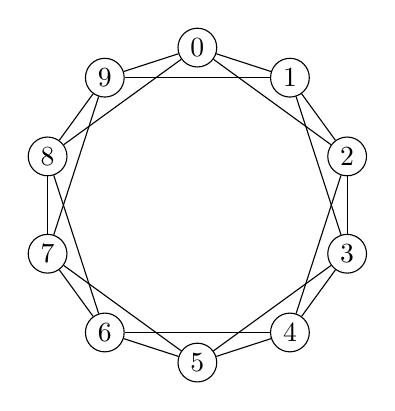
\begin{tikzpicture}[rotate=90]
        \tikzstyle{vertex}=[draw,thin,circle,fill=white,minimum size=14pt,inner sep=0pt]

        \draw (-0*360/10:2) node[vertex] (v1) {0};
        \draw (-1*360/10:2) node[vertex] (v2) {1};
        \draw (-2*360/10:2) node[vertex] (v3) {2};
        \draw (-3*360/10:2) node[vertex] (v4) {3};
        \draw (-4*360/10:2) node[vertex] (v5) {4};
        \draw (-5*360/10:2) node[vertex] (v6) {5};
        \draw (-6*360/10:2) node[vertex] (v7) {6};
        \draw (-7*360/10:2) node[vertex] (v8) {7};
        \draw (-8*360/10:2) node[vertex] (v9) {8};
        \draw (-9*360/10:2) node[vertex] (v10) {9};

        \draw (v2) -- (v1);
        \draw (v3) -- (v1);
        \draw (v3) -- (v2);
        \draw (v4) -- (v2);
        \draw (v4) -- (v3);
        \draw (v5) -- (v3);
        \draw (v5) -- (v4);
        \draw (v6) -- (v4);
        \draw (v6) -- (v5);
        \draw (v7) -- (v5);
        \draw (v7) -- (v6);
        \draw (v8) -- (v6);
        \draw (v8) -- (v7);
        \draw (v9) -- (v1);
        \draw (v9) -- (v7);
        \draw (v9) -- (v8);
        \draw (v10) -- (v1);
        \draw (v10) -- (v2);
        \draw (v10) -- (v8);
        \draw (v10) -- (v9);

    \end{tikzpicture}
    \caption{Cayley Graph of $(Z_{10})$ with the generating set $S= \{\pm 1, \pm 2 \}$}
    \label{fig:z10}
\end{figure}

\end{example}
\newpage

\begin{example}
Figure \ref{fig:D10} shows the Cayley graph of $D_{10}$ with the generating set $S= \{F, R, FR^{-1}\}$. 

 \begin{figure}[H]
\centering
    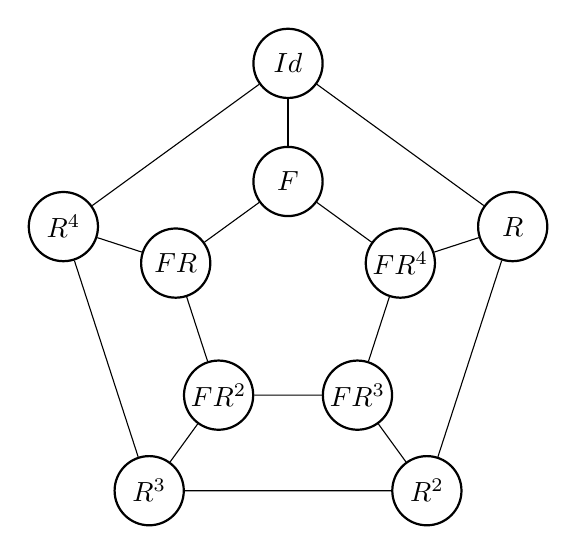
\begin{tikzpicture}[rotate=90,scale=1.5]
        \tikzstyle{vertex}=[draw,thick,circle,fill=white!60,minimum size=25pt,inner sep=0pt]

        \draw (-0*360/5:1) node[vertex] (v1) {$F$};
        \draw (-0*360/5:2) node[vertex] (v2) {$Id$};
        \draw (-1*360/5:1) node[vertex] (v3) {$FR^4$};
        \draw (-1*360/5:2) node[vertex] (v4) {$R$};
        \draw (-2*360/5:1) node[vertex] (v5) {$FR^3$};
        \draw (-2*360/5:2) node[vertex] (v6) {$R^2$};
        \draw (-3*360/5:1) node[vertex] (v7) {$FR^2$};
        \draw (-3*360/5:2) node[vertex] (v8) {$R^3$};
        \draw (-4*360/5:1) node[vertex] (v9) {$FR$};
        \draw (-4*360/5:2) node[vertex] (v10) {$R^4$};

        \draw (v2) -- (v1);
        \draw (v3) -- (v1);
        \draw (v4) -- (v2);
        \draw (v4) -- (v3);
        \draw (v5) -- (v3);
        \draw (v6) -- (v4);
        \draw (v6) -- (v5);
        \draw (v7) -- (v5);
        \draw (v8) -- (v6);
        \draw (v8) -- (v7);
        \draw (v9) -- (v1);
        \draw (v9) -- (v7);
        \draw (v10) -- (v2);
        \draw (v10) -- (v8);
        \draw (v10) -- (v9);
    \end{tikzpicture}
    \caption{Cayley Graph of $D_{10}$ with the generating set $S= \{F, R, FR^{-1}\}$}
    \label{fig:D10}
\end{figure}

\end{example}


My definition of a group operation with the group $(G_{2x2x2}, \scriptstyle * )$ and the set $C$ is : \\
If the Rubik's cube is in a configuration $C=(\sigma, x)$, making a move $M \in G_{2x2x2}$ will bring the cube into a new configuration  $C \cdot M$. 
\\
%Definition of a group operation with the group $(G_{2x2x2}, \scriptstyle*)$ and the set $C$:
%\begin{itemize}
%\item $ C \times G_{2x2x2} \rightarrow C$ with $(c, g) %\rightarrow c \cdot g $ [\textbf{Closure}]
%\item $c \cdot N = x$ for all $c \in C$ and the identity element $N \in G_{2x2x2}$ [\textbf{Identity}]
%\item $c \cdot (u \cdot v) = (c \cdot h) \cdot v$ for all $u, v \in G_{2x2x2}$ and $c \in C$ [\textbf{Associativity}]
%\end{itemize}
% \\
Suppose, the cube is in configuration $C$. Now when the move $M_1 \in G_{2x2x2}$ is made, the new configuration of the cube is $C \cdot M_1$. If another move $M_2 \in G_{2x2x2}$ is made, the new configuration of the cube is $(C \cdot M_1) \cdot M_2$. 
In other words: The cube started in configuration $C$ and the move $M_1 M_2$ was executed. I can also write the new configuration as $C \cdot (M_1 M_2)$ and therefore $(C \cdot M_1) \cdot M_2 = C \cdot (M_1 M_2)$. 

When we make the identity move $N$, the configuration of the cube is not changed. So $C \cdot N = C$. 
\\
In this case, the moves of the cube affect the configuration of the cube. 
%This is a right-hand operation because the elements of the group are on the right.
With Cayley graphs,  we'll have a group whose elements are the nodes of the graph. Here, the nodes of the graph are the elements of the group $(G_{2x2x2}, \scriptstyle*)$ and thus all possible moves. The edges correspond to the valid configurations of the cube, i.e. the set $C$. 

According to the paper \cite{cayleyrubik}, the Cayley graph of \Ttwo cube has $36, 74,160$ nodes which was computed on SUN-3 with 8 megabytes of storage in less than 60 CPU hours.





For more interesting Cayley graphs and deciphering the hidden beauties of finite groups [broadly speaking abstract algebra], one should definitely check this very beautiful paper by Matthew Macauley \cite{macauley2024revealing}. 

\newpage
\section{Transition Functions of the Alignment Vector $\pmb{x}$}

\label{Appendix_AlignmentFunctions}

The following shows that the vector $x$ returns to its initial state after executing one of the basic moves four times. Here $(\sigma, x)$ is any cube configuration. In this section, only the alignment vector $x$ is considered. The corresponding justification for $\sigma$ can be found in section \ref{Section_EqualityOfmoves}.
\begin{align*}
\forall \ Z \in \{U, D, R, L, F, B\} \ . \ (\sigma, x) \cdot Z^4 = (\sigma, x)
\end{align*}


The vector is changed by the function $\gamma$. This function was defined for each of the basic moves in section \ref{Section_AlignmentOfcubies}.

First, the change in the vector $x$ is examined using the move $R$ as an example. The following figures show the transition functions of the vector entries in the cube:
\begin{figure}[H]
\centering
\includegraphics[scale=0.155]{Rhoch1.jpg}
\caption{Vector $x$ to $\gamma_R(x)$}
\end{figure}

\begin{figure}[H]
\centering
\includegraphics[scale=0.155]{Rhoch2.jpg}
\caption{Vector $x$ to $\gamma_R (\gamma_R(x))$}
\end{figure}
\begin{figure}[H]
\centering
\includegraphics[scale=0.155]{Rhoch3.jpg}
\caption{Vector $x$ to $\gamma_R ( \gamma_R (\gamma_R(x)))$}
\end{figure}
\begin{figure}[H]
\centering
\includegraphics[scale=0.155]{Rhoch4.jpg}
\caption{Vector $x$ to $\gamma_R ( \gamma_R ( \gamma_R (\gamma_R(x))))$}
\end{figure}

Below, we can see the change in vector $x$ caused by the move $R^4$. The functions $g$ and $h$ are also nested when $\gamma_R$ is nested.
\begin{align*}
& \gamma_R (\gamma_R (\gamma_R (\gamma_R ((x_1, x_2, x_3, x_4, x_5, x_6, x_7, x_8  )))) \\
& =  (x_1, \ g(h(g(h(x_2)))), \ x_3, \ h(g(h(g(x_4)))), \ x_5, \ h(g(h(g(x_6)))), \ x_7, \ g(h(g(h(x_8)))) )
\end{align*}
The other basic moves change the vector as follows when executed four times:
\begin{align*}
& \gamma_U ( \gamma_U ( \gamma_U ( \gamma_U \left( (x_1, x_2, x_3, x_4, x_5, x_6, x_7, x_8  ) \right) ) ) ) \\ 
& =  \left((x_1, x_2, x_3, x_4, x_5, x_6, x_7, x_8  ) \right) \\
\\ 
& \gamma_D ( \gamma_D ( \gamma_D ( \gamma_D \left( (x_1, x_2, x_3, x_4, x_5, x_6, x_7, x_8  ) \right) ) ) ) \\ 
& =  \left((x_1, x_2, x_3, x_4, x_5, x_6, x_7, x_8  ) \right) \\
\\ 
& \gamma_R (\gamma_R (\gamma_R (\gamma_R ((x_1, x_2, x_3, x_4, x_5, x_6, x_7, x_8  )))) \\
& =  (x_1, \ g(h(g(h(x_2)))), \ x_3, \ h(g(h(g(x_4)))), \ x_5, \ h(g(h(g(x_6)))), \ x_7, \ g(h(g(h(x_8)))) ) \\
\\
& \gamma_L \left( (x_1, x_2, x_3, x_4, x_5, x_6, x_7, x_8  ) \right) \\ 
& =  \left( (h(g(h(g(x_1)))), x_2, g(h(g(h(x_3)))), x_4, g(h(g(h(x_5)))), x_6, h(g(h(g(x_7)))), x_8) \right) \\ 
\\
& \gamma_F \left( (x_1, x_2, x_3, x_4, x_5, x_6, x_7, x_8  ) \right) \\ 
& =  \left( x_1, x_2, h(g(h(g(x_3)))), g(h(g(h(x_4)))), x_5, x_6, g(h(g(h(x_7)))), h(g(h(g(x_8)))) \right) \\
\\
& \gamma_B \left( (x_1, x_2, x_3, x_4, x_5, x_6, x_7, x_8  ) \right) \\ 
& =  \left( g(h(g(h(x_1)))), h(g(h(g(x_2)))), x_3, x_4, h(g(h(g(x_5)))), g(h(g(h(x_6)))), x_7, x_8 \right)
\end{align*}
It can be seen that the changes when the same move is executed four times always consist of the function nestings $g(h(g(h(x))))$ and $h(g(h(g(x))))$. \textbf{Therefore the following must be shown}:
\begin{minipage}[H]{0.5\textwidth}
	\begin{align*}
		g(h(g(h(x)))) = x
	\end{align*}
\end{minipage}
\begin{minipage}[H]{0.5\textwidth}
      \begin{align*}
			h(g(h(g(x)))) = x
	  \end{align*}
\end{minipage}

with
\begin{align*}
g(x)=(x + 2) \hspace*{-0.5em} \mod 3 \ \ \ \ \ \ \ \ \ \ \ \ h(x) = (x+1) \hspace*{-0.5em} \mod 3 
\end{align*}
\begin{proofcustom}
To do this, $g(h(x))$ and $h(g(x))$ are first calculated.

      \begin{align*}
		 & g(h(x)) \\
		= \ & g((x+1) \hspace*{-0.5em} \mod 3) \\
		= \ & ((x+1) \hspace*{-0.5em} \mod 3) +2 \hspace*{-0.5em} \mod 3  \\
		= \ & (x \hspace*{-0.5em} \mod 3) +1 +2 \hspace*{-0.5em} \mod 3  \\
		= \ & (x \hspace*{-0.5em} \mod 3) +3 \hspace*{-0.5em} \mod 3  \\
		= \ & ((x \hspace*{-0.5em} \mod 3) \hspace*{-0.5em} \mod 3  \\
		= \ & x \hspace*{-0.5em} \mod 3 \\
		= \ & x \\
	\end{align*}


      \begin{align*}
		 & h(g(x)) \\
		= \ & h((x+2) \hspace*{-0.5em} \mod 3) \\
		= \ & ((x+2) \hspace*{-0.5em} \mod 3) +1 \hspace*{-0.5em} \mod 3  \\
		= \ & (x \hspace*{-0.5em} \mod 3) +2 +1 \hspace*{-0.5em} \mod 3  \\
		= \ & (x \hspace*{-0.5em} \mod 3) +3 \hspace*{-0.5em} \mod 3  \\
		= \ & ((x \hspace*{-0.5em} \mod 3) \hspace*{-0.5em} \mod 3  \\
		= \ & x \hspace*{-0.5em} \mod 3 \\
		= \ & x \\
	\end{align*}
\end{proofcustom}
The expression $(x \hspace*{-0.5em} \mod 3)$ can be transformed into $x$ in this case, since $x \in \{0,1,2\}$.

Since, $g(h(x))=x$ and $h(g(x))=x$, the following also holds:
\begin{align*}
		g(h(g(h(x)))) = g(h(x)) = x \\
			h(g(h(g(x)))) = h(g(x)) = x \\
	  \end{align*}

Thus, for any cube configuration $(\sigma, x)$:
\begin{align*}
\forall \ Z \in \{U, D, R, L, F, B\} \ . \ (\sigma, x) \cdot Z^4 = (\sigma, x)
\end{align*}
This means that the following also applies to any cube configuration $(\sigma, x)$:
\begin{align*}
\forall \ Z \in \{U, D, R, L, F, B\}, n \in \mathbb{N}, n \hspace*{-0.5em} \mod 4 = 0 \ . \ (\sigma, x) \cdot Z^n = (\sigma, x)
\end{align*}

Accordingly, the move $Z^4$ or $Z^n$ (with $n \hspace*{-0.5em} \mod 4$ and one-element moves $Z$) is a representative of the equivalence class of the empty move and is therefore also a way to form the identity element $N$ of the group $(\Gtwo, \mathlarger{\scriptstyle*})$.

This also applies analogously to the rotations of the cube. In section, \ref{Section_RotationOfCube} the cube rotations were defined by two face rotations each. These are opposite layers that do not affect the same cubies. 
\newpage The quadruple rotations of the cube are defined as face rotations below:
\begin{alignat*}{4}
& Z_lZ_lZ_lZ_l && \Leftrightarrow \ \ &&  DDDD  && \ U^{-1} U^{-1} U^{-1} U^{-1} \\
& Z_rZ_rZ_rZ_r && \Leftrightarrow &&   UUUU  && D^{-1}D^{-1}D^{-1}D^{-1}\\
& Y_lY_lY_lY_l && \Leftrightarrow && LLLL &&  R^{-1}R^{-1}R^{-1}R^{-1} \\
& Y_rY_rY_rY_r && \Leftrightarrow &&  RRRR &&  L^{-1} L^{-1} L^{-1} L^{-1} \\
& X_lX_lX_lX_L && \Leftrightarrow && BBBB &&  F^{-1}F^{-1}F^{-1}F^{-1} \\
& X_rX_rX_rX_r && \Leftrightarrow && FFFF  && B^{-1}B^{-1}B^{-1}B^{-1}   \\
\end{alignat*}

Since all quadruple rotations consist of two quadruple face rotations, the transformations described above can be transferred to the rotations. The vector $x$ therefore remains unchanged even if the same function $\beta$ is executed four times. Thus, for any cube configuration $(\sigma, x)$ also holds:
\begin{align*}
\forall \ W \in \{X_l, X_r, Y_l, Y_r, Z_l, Z_r\} \ . \ (\sigma, x) \cdot W^4 = (\sigma, x)
\end{align*}
\newpage

\section{Data Structures and Algorithms}
\label{DSA}
 \textbf{Data Structures} are structures that are used to handle and store data. Data Structures may be presented by default in a programming language, and if they aren't present in there, we can code them in. Having a good knowledge of data structures is essential as it allows the programmer to be able to manipulate the data as needed seamlessly and effortlessly.\par
\vspace{3.5mm}
An \textbf{algorithm} is a finite set of instructions or logic, written in order, to accomplish a certain predefined task. An algorithm is not the complete code or program, it is just the core solution of a problem, which can be expressed either as an informal high-level description using a flowchart.

\subsubsection*{Pseudo-Code}
Because data structures and algorithms are universally applicable to all languages, it doesn't make sense to talk about the logic in terms of a single programming language. Neither can we just simply state the logic as it may not be understood by everyone. \\
Therefore, to express the logic, we use an informal high-level description of the logic. Furthermore, we can make it so that our descriptions follow the general coding syntax, without actually using a programming language.\\
This informal description of the logic in an algorithm is referred to as \textbf{Pseudo-Code}. 'Pseudo' means "False and is called so because though the description looks like a code, but is not.

\subsection*{Tree}
 Trees are used extensively in the representation of data. They consist of a node, and contain subsequent smaller branches which lead downwards \cite{antunes_time_complexity}. 
\vspace{4mm}
\noindent Some terms related to tree structure:
\begin{itemize}
    \item \textbf{Root:} A node is defined as the start of the structure, also known as a root. This is the entry point to the structure.
    \item \textbf{Children:} Immediate node(s) below the current node.
    \item \textbf{Depth:} Length of the path from the root node to that particular node. The depth of a node can be used to determine its position within the tree and to analyze the structure of the tree.
\begin{example}
The root node is considered to be at depth 0. Its children are at depth 1, their children are at depth 2, and so on. 
\end{example}
    \item \textbf{Ancestor:} All the nodes above the current node.
    \item \textbf{Descendants:} All the nodes below the current node
    \item \textbf{Sibling:} Nodes with the same parent
    \item \textbf{Leaf:} Nodes at the end of a particular path are called leaves. They've no children.
\end{itemize}

 Every node has two associated children, one left and one right. One of these is always smaller than or equal to the parent and the other larger, with the same rule applying across the entire tree. Generally, the left node is smaller.


A \textbf{Binary Tree} is a tree in which each node has a maximum of two sub-nodes. A binary tree is very simple, yet is very powerful.


It was a very short discussion of Data Structure and Algorithm. The topic is very vast and I mostly referred a very part from \cite{bds,fox}.

\newpage
\section{All Rotation Possibilities of the Cube}
\label{Appendix_RotationsOfCube}

Figure \ref{ImageCubeRotationAllSides} shows all rotation possibilities of the cube. 

\begin{figure}[H]
\centering
\includegraphics[scale=0.06]{AllRotations.png}
\caption{Rotation Possibilities of the Cube}
\label{ImageCubeRotationAllSides}
\end{figure}
\newpage
It is the complete illustration of all rotation possibilities of the cube (see figure \ref{ImageCubeRotationAllSides}) and the connections between these possibilities.

\begin{adjustbox}{width=1\textwidth,center}
\begin{tabular}{c | c c c c c c c c c c c c c c c c c c c c c c c c}
\toprule

& $N_R$ & $X_r$ & $Y_r$ & $Z_r$ & $X_l$ & $Y_l$ & $Z_l$ & $X_rX_r$ & $Y_rY_r$ & $Z_rZ_r$ & $X_rY_r$ & $Y_rX_l$ & $X_lY_l$ & $Y_lX_r$ & $Y_lX_l$ & $X_rY_l$ & $Y_rX_r$ & $X_lY_r$ & $X_rY_rZ_r$ & $Y_rZ_rX_r$ & $Y_lX_lZ_l$ & $X_lZ_rY_r$ & $Y_lX_rZ_r$ & $X_lY_lZ_r$ \\

\midrule

$N_R$ & $N_R$ & $X_r$ & $Y_r$ & $Z_r$ & $X_l$ & $Y_l$ & $Z_l$ & $X_rX_r$ & $Y_rY_r$ & $Z_rZ_r$ & $X_rY_r$ & $Y_rX_l$ & $X_lY_l$ & $Y_lX_r$ & $Y_lX_l$ & $X_rY_l$ & $Y_rX_r$ & $X_lY_r$ & $X_rY_rZ_r$ & $Y_rZ_rX_r$ & $Y_rX_lZ_l$ & $X_lZ_rY_r$ & $Y_lX_rZ_r$ & $X_lY_lZ_r$ \\

$X_r$ & $X_r$ & $X_rX_r$ & $Y_rX_r$ & $X_rY_r$ & $N_R$ & $Y_lX_r$ & $X_rY_l$ & $X_l$ & $Y_lX_rZ_r$ & $Y_lX_lZ_l$ & $Y_rZ_rX_r$ & $Y_r$ & $Z_r$ & $X_rY_rZ_r$ & $Y_l$ & $X_lZ_rY_r$ & $X_lY_lZ_r$ & $Z_l$ & $Y_lX_l$ & $X_lY_l$ & $Y_rY_r$ & $X_lY_r$ & $Z_rZ_r$ & $Y_rX_l$ \\

$Y_r$ & $Y_r$ & $X_rY_r$ & $Y_rY_r$ & $Y_rX_l$ & $X_lY_r$ & $N_R$ & $Y_rX_r$ & $X_rY_rZ_r$ & $Y_l$ & $X_lY_lZ_r$ & $Y_lX_lZ_l$ & $X_lZ_rY_r$ & $X_l$ & $Z_r$ & $Z_l$ & $X_r$ & $Y_rZ_rX_r$ & $Y_lX_rZ_r$ & $Z_rZ_r$ & $Y_lX_l$ & $X_rY_l$ & $Y_lX_r$ & $X_lY_l$ & $X_rX_r$ \\

$Z_r$ & $Z_r$ & $Y_lX_r$ & $X_rY_r$ & $Z_rZ_r$ & $Y_rX_l$ & $X_lY_l$ & $N_R$ & $X_lZ_rY_r$ & $Y_rZ_rX_r$ & $Z_l$ & $X_rY_rZ_r$ & $Y_lX_lZ_l$ & $X_lY_lZ_r$ & $Y_lX_rZ_r$ & $X_l$ & $Y_l$ & $X_r$ & $Y_r$ & $X_lY_r$ & $X_rX_r$ & $Y_lX_l$ & $Y_rY_r$ & $Y_rX_r$ & $X_rY_l$ \\

$X_l$ & $X_l$ & $N_R$ & $Y_rX_l$ & $X_lY_l$ & $X_rX_r$ & $Y_lX_l$ & $X_lY_r$ & $X_r$ & $Y_lX_lZ_l$ & $Y_lX_rZ_r$ & $Z_r$ & $X_lY_lZ_r$ & $Y_rZ_rX_r$ & $Y_l$ & $X_rY_rZ_r$ & $Z_l$ & $Y_r$ & $X_lZ_rY_r$ & $Y_lX_r$ & $X_rY_r$ & $Z_rZ_r$ & $X_rY_l$ & $Y_rY_r$ & $Y_rX_r$ \\

$Y_l$ & $Y_l$ & $X_rY_l$ & $N_R$ & $Y_lX_r$ & $X_lY_l$ & $Y_rY_r$ & $Y_lX_l$ & $X_lY_lZ_r$ & $Y_r$ & $X_rY_rZ_r$ & $X_r$ & $Z_r$ & $Y_lX_rZ_r$ & $X_lZ_rY_r$ & $Y_rZ_rX_r$ & $Y_lX_lZ_l$ & $Z_l$ & $X_l$ & $X_rX_r$ & $Y_rX_r$ & $X_rY_r$ & $Y_rX_l$ & $X_lY_r$ & $Z_rZ_r$ \\

$Z_l$ & $Z_l$ & $Y_rX_r$ & $X_lY_r$ & $N_R$ & $Y_lX_l$ & $X_rY_l$ & $Z_rZ_r$ & $Y_rZ_rX_r$ & $X_lZ_rY_r$ & $Z_r$ & $Y_r$ & $X_l$ & $Y_l$ & $X_r$ & $Y_lX_lZ_l$ & $X_lY_lZ_r$ & $Y_lX_rZ_r$ & $X_rY_rZ_r$ & $X_rY_r$ & $Y_rY_r$ & $Y_rX_l$ & $X_rX_r$ & $Y_lX_r$ & $X_lY_l$ \\

$X_rX_r$  & $X_rX_r$ & $X_l$ & $X_lY_lZ_r$ & $Y_rZ_rX_r$ & $X_r$ & $X_rY_rZ_r$ & $X_lZ_rY_r$ & $N_R$ & $Z_rZ_r$ & $Y_rY_r$ & $X_lY_l$ & $Y_rX_r$ & $X_rY_r$ & $Y_lX_l$ & $Y_lX_r$ & $X_lY_r$ & $Y_rX_l$ & $X_rY_l$ & $Y_l$ & $Z_r$ & $Y_lX_rZ_r$ & $Z_l$ & $Y_lX_lZ_l$ & $Y_r$ \\

$Y_rY_r$ & $Y_rY_r$ & $Y_lX_lZ_l$ & $Y_l$ & $X_lZ_rY_r$ & $Y_lX_rZ_r$ & $Y_r$ & $Y_rZ_rX_r$ & $Z_rZ_r$ & $N_R$ & $X_rX_r$ & $X_rY_l$ & $Y_lX_r$ & $X_lY_r$ & $Y_rX_l$ & $Y_rX_r$ & $X_rY_r$ & $Y_lX_l$ & $X_lY_l$ & $X_lY_lZ_r$ & $Z_l$ & $X_r$ & $Z_r$ & $X_l$ & $X_rY_rZ_r$ \\

$Z_rZ_r$ & $Z_rZ_r$ & $Y_lX_rZ_r$ & $X_rY_rZ_r$ & $Z_l$ & $Y_lX_lZ_l$ & $X_lY_lZ_r$ & $Z_r$ & $Y_rY_r$ & $X_rX_r$ & $N_R$ & $X_lY_r$ & $Y_lX_l$ & $X_rY_l$ & $Y_rX_r$ & $Y_rX_l$ & $X_lY_l$ & $Y_lX_r$ & $X_rY_r$ & $Y_r$ & $X_lZ_rY_r$ & $X_l$ & $Y_rZ_rX_r$ & $X_r$ & $Y_l$ \\

$X_rY_r$ & $X_rY_r$ & $X_rY_rZ_r$ & $Y_rZ_rX_r$ & $Y_lX_lZ_l$ & $Y_r$ & $Z_r$ & $X_r$ & $X_lY_r$ & $X_lY_l$ & $X_rY_l$ & $Y_lX_l$ & $Y_rY_r$ & $Y_rX_l$ & $Z_rZ_r$ & $N_R$ & $Y_lX_r$ & $X_rX_r$ & $Y_rX_r$ & $Z_l$ & $X_l$ & $Y_l$ & $Y_lX_rZ_r$ & $X_lY_lZ_r$ & $X_lY_rZ_r$ \\

$Y_rX_l$ & $Y_rX_l$ & $Z_r$ & $Y_lX_lZ_l$ & $X_lY_lZ_r$ & $X_lZ_rY_r$ & $X_l$ & $Y_r$ & $Y_lX_r$ & $Y_lX_l$ & $Y_rX_r$ & $Z_rZ_r$ & $X_rY_l$ & $X_rX_r$ & $X_lY_l$ & $X_lY_r$ & $N_R$ & $X_rY_r$ & $Y_rY_r$ & $Y_lX_rZ_r$ & $X_rY_rZ_r$ & $Z_l$ & $Y_l$ & $Y_rZ_rX_r$ & $X_r$ \\

$X_lY_l$ & $X_lY_l$ & $Y_l$ & $Z_r$ & $Y_lX_rZ_r$ & $X_lY_lZ_r$ & $Y_rZ_rX_r$ & $X_l$ & $X_rY_l$ & $X_rY_r$ & $X_lY_r$ & $Y_lX_r$ & $Z_rZ_r$ & $Y_rX_r$ & $Y_rY_r$ & $X_rX_r$ & $Y_lX_l$ & $N_R$ & $Y_rX_l$ & $X_lZ_rY_r$ & $X_r$ & $X_rY_rZ_r$ & $Y_lX_lZ_l$ & $Y_r$ & $Z_l$ \\

$Y_lX_r$ & $Y_lX_r$ & $X_lZ_rY_r$ & $X_r$ & $X_rY_rZ_r$ & $Z_r$ & $Y_lX_rZ_r$ & $Y_l$ & $Y_rX_l$ & $Y_rX_r$ & $Y_lX_l$ & $X_rX_r$ & $X_rY_r$ & $Z_rZ_r$ & $X_lY_r$ & $X_lY_l$ & $Y_rY_r$ & $X_rY_l$ & $N_R$ & $X_l$ & $X_lY_lZ_r$ & $Y_rZ_rX_r$ & $Y_r$ & $Z_l$ & $Y_lX_lZ_l$ \\

$Y_lX_l$ & $Y_lX_l$ & $Z_l$ & $X_l$ & $Y_l$ & $Y_rZ_rX_r$ & $Y_lX_lZ_l$ & $X_rY_rZ_r$ & $Y_rX_r$ & $Y_rX_l$ & $Y_lX_r$ & $N_R$ & $X_lY_l$ & $Y_rY_r$ & $X_rY_l$ & $X_rY_r$ & $Z_rZ_r$ & $X_lY_r$ & $X_rX_r$ & $X_r$ & $Y_r$ & $Z_r$ & $X_lY_lZ_r$ & $X_lZ_rY_R$ & $Y_lX_rZ_r$ \\

$X_rY_l$ & $X_rY_l$ & $X_lY_lZ_r$ & $Z_l$ & $X_r$ & $Y_l$ & $X_lZ_rY_r$ & $Y_lX_lZ_l$ & $X_lY_l$ & $X_lY_r$ & $X_rY_r$ & $Y_rX_r$ & $N_R$ & $Y_lX_r$ & $X_rX_r$ & $Y_rY_r$ & $Y_rX_l$ & $Z_rZ_r$ & $Y_lX_l$ & $Y_rZ_rX_r$ & $Y_lX_rZ_r$ & $Y_r$ & $X_l$ & $X_rY_rZ_r$ & $Z_r$ \\

$Y_rX_r$ & $Y_rX_r$ & $Y_rZ_rX_r$ & $Y_lX_rZ_r$ & $Y_r$ & $Z_l$ & $X_r$ & $X_lY_lZ_r$ & $Y_lX_l$ & $Y_lX_r$ & $Y_rX_l$ & $Y_rY_r$ & $X_lY_r$ & $N_R$ & $X_rY_r$ & $X_rY_l$ & $X_rX_r$ & $X_lY_l$ & $Z_rZ_r$ & $Y_lX_lZ_l$ & $Y_l$ & $X_lZ_rY_r$ & $X_rY_rZ_r$ & $Z_r$ & $Y_r$ \\

$X_lY_r$ & $X_rY_r$ & $Y_r$ & $X_lZ_rY_r$ & $X_l$ & $X_rY_rZ_r$ & $Z_l$ & $Y_lX_rZ_r$ & $X_rY_r$ & $X_rY_l$ & $X_lY_l$ & $Y_rX_l$ & $X_rX_r$ & $Y_lX_l$ & $N_R$ & $Z_rZ_r$ & $Y_rX_r$ & $Y_rY_r$ & $Y_lX_r$ & $Z_r$ & $Y_lX_lZ_l$ & $X_lY_lZ_r$ & $X_r$ & $Y_l$ & $Y_rZ_rX_r$ \\

$X_rY_rZ_r$ & $X_rY_rZ_r$ & $X_lY_r$ & $X_rX_r$ & $Y_lX_l$ & $X_rY_r$ & $Z_rZ_r$ & $Y_lX_r$ & $Y_r$ & $X_lY_lZ_r$ & $Y_l$ & $X_l$ & $Y_rZ_rX_r$ & $Y_lX_lZ_l$ & $Z_l$ & $Z_r$ & $Y_lX_rZ_r$ & $X_lZ_rY_r$ & $X_r$ & $N_R$ & $Y_rX_l$ & $X_lY_l$ & $Y_rX_r$ & $X_lY_l$ & $Y_rY_r$ \\

$Y_rZ_rX_r$ & $Y_rZ_rX_r$ & $Y_lX_l$ & $X_lY_l$ & $Y_rY_r$ & $Y_rX_r$ & $X_rY_r$ & $X_rX_r$ & $Z_l$ & $Z_r$ & $X_lZ_rY_r$ & $Y_l$ & $Y_lX_rZ_r$ & $Y_r$ & $Y_lX_lZ_l$ & $X_r$ & $X_rY_rZ_r$ & $X_l$ & $X_lY_lZ_r$ & $X_rY_l$ & $N_R$ & $Y_lX_r$ & $Z_rZ_r$ & $Y_rX_l$ & $X_lY_r$ \\

$Y_lX_lZ_l$ & $Y_rX_lZ_l$ & $Z_rZ_r$ & $Y_lX_l$ & $X_rY_l$ & $Y_rY_r$ & $Y_rX_l$ & $X_rY_r$ & $Y_lX_rZ_r$ & $X_l$ & $X_r$ & $Z_l$ & $Y_l$ & $X_lZ_rY_r$ & $X_lY_lZ_r$ & $Y_r$ & $Z_r$ & $X_rY_rZ_r$ & $Y_rZ_rX_r$ & $Y_rX_r$ & $X_lY_r$ & $N_R$ & $X_lY_l$ & $X_rX_r$ & $Y_lX_r$ \\

$X_lZ_rY_r$ & $X_lZ_rY_r$ & $Y_rX_l$ & $X_rY_l$ & $X_rX_r$ & $Y_lX_r$ & $X_lY_r$ & $Y_rY_r$ & $Z_r$ & $Z_l$ & $Y_rZ_rX_r$ & $X_lY_lZ_r$ & $X_r$ & $X_rY_rZ_r$ & $X_l$ & $Y_lX_rZ_r$ & $Y_r$ & $Y_lX_lZ_l$ & $Y_l$ & $X_lY_l$ & $Z_rZ_r$ & $Y_rX_r$ & $N_R$ & $Y_lX_l$ & $X_rY_r$ \\

$Y_lX_rZ_r$ & $Y_lX_rZ_r$ & $Y_rY_r$ & $Y_lX_r$ & $X_lY_r$ & $Z_rZ_r$ & $Y_rX_r$ & $X_lY_l$ & $Y_lX_lZ_l$ & $X_r$ & $X_l$ & $X_lZ_rY_r$ & $X_rY_rZ_r$ & $Z_l$ & $Y_r$ & $x_lY_lU_r$ & $Y_rZ_rX_r$ & $Y_l$ & $Z_r$ & $Y_rX_l$ & $X_rY_l$ & $X_rX_r$ & $X_rY_r$ & $N_R$ & $Y_lX_l$ \\

$X_lY_lZ_r$ & $X_lY_lZ_r$ & $X_lY_l$ & $Z_rZ_r$ & $Y_rX_r$ & $X_rY_l$ & $X_rX_r$ & $Y_rX_l$ & $Y_l$ & $X_rY_rZ_r$ & $Y_r$ & $Y_lX_rZ_r$ & $Z_l$ & $X_r$ & $Y_rZ_rX_r$ & $X_lZ_rY_r$ & $X_l$ & $Z_r$ & $Y_lX_lZ_l$ & $Y_rY_r$ & $Y_lX_r$ & $X_lY_r$ & $Y_lX_l$ & $X_rY_r$ & $N_R$ \\



\bottomrule
\end{tabular}

\end{adjustbox}
\ 




\begin{note}
    This table reads in such a way that the rotation above the column is carried out first and then the rotation of the corresponding row.  From the table, we can also observe that a maximum of three rotations can be lined up. The length of the rotations then decreases again.
\end{note}
\newpage

%\bibliography{references}
%\bibliographystyle{unsrt}
\printbibliography

\end{document}
